\documentclass[twoside]{book}

% Packages required by doxygen
\usepackage{fixltx2e}
\usepackage{calc}
\usepackage{doxygen}
\usepackage[export]{adjustbox} % also loads graphicx
\usepackage{graphicx}
\usepackage[utf8]{inputenc}
\usepackage{makeidx}
\usepackage{multicol}
\usepackage{multirow}
\PassOptionsToPackage{warn}{textcomp}
\usepackage{textcomp}
\usepackage[nointegrals]{wasysym}
\usepackage[table]{xcolor}

% Font selection
\usepackage[T1]{fontenc}
\usepackage[scaled=.90]{helvet}
\usepackage{courier}
\usepackage{amssymb}
\usepackage{sectsty}
\renewcommand{\familydefault}{\sfdefault}
\allsectionsfont{%
  \fontseries{bc}\selectfont%
  \color{darkgray}%
}
\renewcommand{\DoxyLabelFont}{%
  \fontseries{bc}\selectfont%
  \color{darkgray}%
}
\newcommand{\+}{\discretionary{\mbox{\scriptsize$\hookleftarrow$}}{}{}}

% Page & text layout
\usepackage{geometry}
\geometry{%
  a4paper,%
  top=2.5cm,%
  bottom=2.5cm,%
  left=2.5cm,%
  right=2.5cm%
}
\tolerance=750
\hfuzz=15pt
\hbadness=750
\setlength{\emergencystretch}{15pt}
\setlength{\parindent}{0cm}
\setlength{\parskip}{3ex plus 2ex minus 2ex}
\makeatletter
\renewcommand{\paragraph}{%
  \@startsection{paragraph}{4}{0ex}{-1.0ex}{1.0ex}{%
    \normalfont\normalsize\bfseries\SS@parafont%
  }%
}
\renewcommand{\subparagraph}{%
  \@startsection{subparagraph}{5}{0ex}{-1.0ex}{1.0ex}{%
    \normalfont\normalsize\bfseries\SS@subparafont%
  }%
}
\makeatother

% Headers & footers
\usepackage{fancyhdr}
\pagestyle{fancyplain}
\fancyhead[LE]{\fancyplain{}{\bfseries\thepage}}
\fancyhead[CE]{\fancyplain{}{}}
\fancyhead[RE]{\fancyplain{}{\bfseries\leftmark}}
\fancyhead[LO]{\fancyplain{}{\bfseries\rightmark}}
\fancyhead[CO]{\fancyplain{}{}}
\fancyhead[RO]{\fancyplain{}{\bfseries\thepage}}
\fancyfoot[LE]{\fancyplain{}{}}
\fancyfoot[CE]{\fancyplain{}{}}
\fancyfoot[RE]{\fancyplain{}{\bfseries\scriptsize Generated by Doxygen }}
\fancyfoot[LO]{\fancyplain{}{\bfseries\scriptsize Generated by Doxygen }}
\fancyfoot[CO]{\fancyplain{}{}}
\fancyfoot[RO]{\fancyplain{}{}}
\renewcommand{\footrulewidth}{0.4pt}
\renewcommand{\chaptermark}[1]{%
  \markboth{#1}{}%
}
\renewcommand{\sectionmark}[1]{%
  \markright{\thesection\ #1}%
}

% Indices & bibliography
\usepackage{natbib}
\usepackage[titles]{tocloft}
\setcounter{tocdepth}{3}
\setcounter{secnumdepth}{5}
\makeindex

% Hyperlinks (required, but should be loaded last)
\usepackage{ifpdf}
\ifpdf
  \usepackage[pdftex,pagebackref=true]{hyperref}
\else
  \usepackage[ps2pdf,pagebackref=true]{hyperref}
\fi
\hypersetup{%
  colorlinks=true,%
  linkcolor=blue,%
  citecolor=blue,%
  unicode%
}

% Custom commands
\newcommand{\clearemptydoublepage}{%
  \newpage{\pagestyle{empty}\cleardoublepage}%
}

\usepackage{caption}
\captionsetup{labelsep=space,justification=centering,font={bf},singlelinecheck=off,skip=4pt,position=top}

%===== C O N T E N T S =====

\begin{document}

% Titlepage & ToC
\hypersetup{pageanchor=false,
             bookmarksnumbered=true,
             pdfencoding=unicode
            }
\pagenumbering{alph}
\begin{titlepage}
\vspace*{7cm}
\begin{center}%
{\Large P\+AD Game Engine }\\
\vspace*{1cm}
{\large Generated by Doxygen 1.8.14}\\
\end{center}
\end{titlepage}
\clearemptydoublepage
\pagenumbering{roman}
\tableofcontents
\clearemptydoublepage
\pagenumbering{arabic}
\hypersetup{pageanchor=true}

%--- Begin generated contents ---
\chapter{P\+A\+D-\/\+Game-\/\+Engine}
\label{md__r_e_a_d_m_e}
\Hypertarget{md__r_e_a_d_m_e}
A custom made c++ engine from scratch, with Open\+GL, Qt and Bullet library. 
\chapter{Namespace Index}
\section{Namespace List}
Here is a list of all namespaces with brief descriptions\+:\begin{DoxyCompactList}
\item\contentsline{section}{\mbox{\hyperlink{namespacepad}{pad}} }{\pageref{namespacepad}}{}
\item\contentsline{section}{\mbox{\hyperlink{namespacepad_1_1core}{pad\+::core}} }{\pageref{namespacepad_1_1core}}{}
\item\contentsline{section}{\mbox{\hyperlink{namespacepad_1_1gfx}{pad\+::gfx}} }{\pageref{namespacepad_1_1gfx}}{}
\item\contentsline{section}{\mbox{\hyperlink{namespacepad_1_1math}{pad\+::math}} }{\pageref{namespacepad_1_1math}}{}
\item\contentsline{section}{\mbox{\hyperlink{namespacepad_1_1sys}{pad\+::sys}} }{\pageref{namespacepad_1_1sys}}{}
\end{DoxyCompactList}

\chapter{Hierarchical Index}
\section{Class Hierarchy}
This inheritance list is sorted roughly, but not completely, alphabetically\+:\begin{DoxyCompactList}
\item \contentsline{section}{pad\+:\+:core\+:\+:Engine}{\pageref{classpad_1_1core_1_1_engine}}{}
\item \contentsline{section}{pad\+:\+:core\+:\+:Engine\+Clock}{\pageref{classpad_1_1core_1_1_engine_clock}}{}
\item \contentsline{section}{pad\+:\+:sys\+:\+:I\+Module}{\pageref{classpad_1_1sys_1_1_i_module}}{}
\begin{DoxyCompactList}
\item \contentsline{section}{pad\+:\+:gfx\+:\+:Renderer}{\pageref{classpad_1_1gfx_1_1_renderer}}{}
\end{DoxyCompactList}
\item \contentsline{section}{pad\+:\+:sys\+:\+:I\+Window\+Base}{\pageref{classpad_1_1sys_1_1_i_window_base}}{}
\begin{DoxyCompactList}
\item \contentsline{section}{pad\+:\+:sys\+:\+:S\+D\+L\+Window}{\pageref{classpad_1_1sys_1_1_s_d_l_window}}{}
\end{DoxyCompactList}
\item \contentsline{section}{pad\+:\+:math\+:\+:Matrix4x4}{\pageref{structpad_1_1math_1_1_matrix4x4}}{}
\item \contentsline{section}{pad\+:\+:gfx\+:\+:Render\+Settings}{\pageref{structpad_1_1gfx_1_1_render_settings}}{}
\item \contentsline{section}{pad\+:\+:gfx\+:\+:Shader}{\pageref{classpad_1_1gfx_1_1_shader}}{}
\item \contentsline{section}{pad\+:\+:core\+:\+:Timer}{\pageref{classpad_1_1core_1_1_timer}}{}
\item \contentsline{section}{pad\+:\+:math\+:\+:Vector2$<$ T $>$}{\pageref{structpad_1_1math_1_1_vector2}}{}
\item \contentsline{section}{pad\+:\+:math\+:\+:Vector3$<$ T $>$}{\pageref{structpad_1_1math_1_1_vector3}}{}
\item \contentsline{section}{pad\+:\+:math\+:\+:Vector4$<$ T $>$}{\pageref{structpad_1_1math_1_1_vector4}}{}
\item \contentsline{section}{pad\+:\+:sys\+:\+:Window\+Settings}{\pageref{structpad_1_1sys_1_1_window_settings}}{}
\end{DoxyCompactList}

\chapter{Class Index}
\section{Class List}
Here are the classes, structs, unions and interfaces with brief descriptions\+:\begin{DoxyCompactList}
\item\contentsline{section}{\mbox{\hyperlink{classpad_1_1core_1_1_engine}{pad\+::core\+::\+Engine}} }{\pageref{classpad_1_1core_1_1_engine}}{}
\item\contentsline{section}{\mbox{\hyperlink{structpad_1_1math_1_1_vector2}{pad\+::math\+::\+Vector2$<$ T $>$}} }{\pageref{structpad_1_1math_1_1_vector2}}{}
\item\contentsline{section}{\mbox{\hyperlink{structpad_1_1math_1_1_vector3}{pad\+::math\+::\+Vector3$<$ T $>$}} }{\pageref{structpad_1_1math_1_1_vector3}}{}
\item\contentsline{section}{\mbox{\hyperlink{structpad_1_1math_1_1_vector4}{pad\+::math\+::\+Vector4$<$ T $>$}} }{\pageref{structpad_1_1math_1_1_vector4}}{}
\end{DoxyCompactList}

\chapter{File Index}
\section{File List}
Here is a list of all files with brief descriptions\+:\begin{DoxyCompactList}
\item\contentsline{section}{Math/\+Sources/\mbox{\hyperlink{_vector2_8h}{Vector2.\+h}} }{\pageref{_vector2_8h}}{}
\item\contentsline{section}{Math/\+Sources/\mbox{\hyperlink{_vector2__impl_8h}{Vector2\+\_\+impl.\+h}} }{\pageref{_vector2__impl_8h}}{}
\item\contentsline{section}{Math/\+Sources/\mbox{\hyperlink{_vector3_8h}{Vector3.\+h}} }{\pageref{_vector3_8h}}{}
\item\contentsline{section}{Math/\+Sources/\mbox{\hyperlink{_vector3__impl_8h}{Vector3\+\_\+impl.\+h}} }{\pageref{_vector3__impl_8h}}{}
\item\contentsline{section}{Math/\+Sources/\mbox{\hyperlink{_vector4_8h}{Vector4.\+h}} }{\pageref{_vector4_8h}}{}
\item\contentsline{section}{Math/\+Sources/\mbox{\hyperlink{_vector4__impl_8h}{Vector4\+\_\+impl.\+h}} }{\pageref{_vector4__impl_8h}}{}
\item\contentsline{section}{P\+A\+D Engine/\mbox{\hyperlink{_main_8cpp}{Main.\+cpp}} }{\pageref{_main_8cpp}}{}
\item\contentsline{section}{P\+A\+D Engine/\+Sources/\mbox{\hyperlink{_sources_2_main_8cpp}{Main.\+cpp}} }{\pageref{_sources_2_main_8cpp}}{}
\item\contentsline{section}{P\+A\+D Engine/\+Sources/\+Core/\mbox{\hyperlink{_engine_8cpp}{Engine.\+cpp}} }{\pageref{_engine_8cpp}}{}
\item\contentsline{section}{P\+A\+D Engine/\+Sources/\+Core/\mbox{\hyperlink{_engine_8h}{Engine.\+h}} }{\pageref{_engine_8h}}{}
\end{DoxyCompactList}

\chapter{Namespace Documentation}
\hypertarget{namespacepad}{}\section{pad Namespace Reference}
\label{namespacepad}\index{pad@{pad}}
\subsection*{Namespaces}
\begin{DoxyCompactItemize}
\item 
 \mbox{\hyperlink{namespacepad_1_1core}{core}}
\item 
 \mbox{\hyperlink{namespacepad_1_1gfx}{gfx}}
\item 
 \mbox{\hyperlink{namespacepad_1_1math}{math}}
\item 
 \mbox{\hyperlink{namespacepad_1_1sys}{sys}}
\end{DoxyCompactItemize}
\subsection*{Typedefs}
\begin{DoxyCompactItemize}
\item 
using \mbox{\hyperlink{namespacepad_a9f598447cac2137f85ac7bb9322fe6be}{int8}} = char
\item 
using \mbox{\hyperlink{namespacepad_ac2d92bf238fe849ef0eab976bc6f6040}{uint8}} = unsigned char
\item 
using \mbox{\hyperlink{namespacepad_ab1a45c1f61489add8bf3a4c7a563d67a}{int16}} = short
\item 
using \mbox{\hyperlink{namespacepad_a03b9241a5f6a191da2faac64714e1038}{uint16}} = unsigned short
\item 
using \mbox{\hyperlink{namespacepad_a7faacd72761782d8adef66f2feba3c21}{int32}} = int
\item 
using \mbox{\hyperlink{namespacepad_a4101021f78334c7c461eef5b0b2eaa6f}{uint32}} = unsigned int
\item 
using \mbox{\hyperlink{namespacepad_a91b3934f581b6b83d2618e069a120fdd}{int64}} = long long int
\item 
using \mbox{\hyperlink{namespacepad_ae548145eb697683a147ccccabd88c77c}{uint64}} = unsigned long long int
\item 
using \mbox{\hyperlink{namespacepad_a0620ec4561a638bdbef1530ccf90fd4b}{float32}} = float
\item 
using \mbox{\hyperlink{namespacepad_a0b20ee3154cbe817a8d34c9e4b3b0508}{float64}} = double
\end{DoxyCompactItemize}


\subsection{Typedef Documentation}
\mbox{\Hypertarget{namespacepad_a0620ec4561a638bdbef1530ccf90fd4b}\label{namespacepad_a0620ec4561a638bdbef1530ccf90fd4b}} 
\index{pad@{pad}!float32@{float32}}
\index{float32@{float32}!pad@{pad}}
\subsubsection{\texorpdfstring{float32}{float32}}
{\footnotesize\ttfamily using \mbox{\hyperlink{namespacepad_a0620ec4561a638bdbef1530ccf90fd4b}{pad\+::float32}} = typedef float}

\mbox{\Hypertarget{namespacepad_a0b20ee3154cbe817a8d34c9e4b3b0508}\label{namespacepad_a0b20ee3154cbe817a8d34c9e4b3b0508}} 
\index{pad@{pad}!float64@{float64}}
\index{float64@{float64}!pad@{pad}}
\subsubsection{\texorpdfstring{float64}{float64}}
{\footnotesize\ttfamily using \mbox{\hyperlink{namespacepad_a0b20ee3154cbe817a8d34c9e4b3b0508}{pad\+::float64}} = typedef double}

\mbox{\Hypertarget{namespacepad_ab1a45c1f61489add8bf3a4c7a563d67a}\label{namespacepad_ab1a45c1f61489add8bf3a4c7a563d67a}} 
\index{pad@{pad}!int16@{int16}}
\index{int16@{int16}!pad@{pad}}
\subsubsection{\texorpdfstring{int16}{int16}}
{\footnotesize\ttfamily using \mbox{\hyperlink{namespacepad_ab1a45c1f61489add8bf3a4c7a563d67a}{pad\+::int16}} = typedef short}

\mbox{\Hypertarget{namespacepad_a7faacd72761782d8adef66f2feba3c21}\label{namespacepad_a7faacd72761782d8adef66f2feba3c21}} 
\index{pad@{pad}!int32@{int32}}
\index{int32@{int32}!pad@{pad}}
\subsubsection{\texorpdfstring{int32}{int32}}
{\footnotesize\ttfamily using \mbox{\hyperlink{namespacepad_a7faacd72761782d8adef66f2feba3c21}{pad\+::int32}} = typedef int}

\mbox{\Hypertarget{namespacepad_a91b3934f581b6b83d2618e069a120fdd}\label{namespacepad_a91b3934f581b6b83d2618e069a120fdd}} 
\index{pad@{pad}!int64@{int64}}
\index{int64@{int64}!pad@{pad}}
\subsubsection{\texorpdfstring{int64}{int64}}
{\footnotesize\ttfamily using \mbox{\hyperlink{namespacepad_a91b3934f581b6b83d2618e069a120fdd}{pad\+::int64}} = typedef long long int}

\mbox{\Hypertarget{namespacepad_a9f598447cac2137f85ac7bb9322fe6be}\label{namespacepad_a9f598447cac2137f85ac7bb9322fe6be}} 
\index{pad@{pad}!int8@{int8}}
\index{int8@{int8}!pad@{pad}}
\subsubsection{\texorpdfstring{int8}{int8}}
{\footnotesize\ttfamily using \mbox{\hyperlink{namespacepad_a9f598447cac2137f85ac7bb9322fe6be}{pad\+::int8}} = typedef char}

\mbox{\Hypertarget{namespacepad_a03b9241a5f6a191da2faac64714e1038}\label{namespacepad_a03b9241a5f6a191da2faac64714e1038}} 
\index{pad@{pad}!uint16@{uint16}}
\index{uint16@{uint16}!pad@{pad}}
\subsubsection{\texorpdfstring{uint16}{uint16}}
{\footnotesize\ttfamily using \mbox{\hyperlink{namespacepad_a03b9241a5f6a191da2faac64714e1038}{pad\+::uint16}} = typedef unsigned short}

\mbox{\Hypertarget{namespacepad_a4101021f78334c7c461eef5b0b2eaa6f}\label{namespacepad_a4101021f78334c7c461eef5b0b2eaa6f}} 
\index{pad@{pad}!uint32@{uint32}}
\index{uint32@{uint32}!pad@{pad}}
\subsubsection{\texorpdfstring{uint32}{uint32}}
{\footnotesize\ttfamily using \mbox{\hyperlink{namespacepad_a4101021f78334c7c461eef5b0b2eaa6f}{pad\+::uint32}} = typedef unsigned int}

\mbox{\Hypertarget{namespacepad_ae548145eb697683a147ccccabd88c77c}\label{namespacepad_ae548145eb697683a147ccccabd88c77c}} 
\index{pad@{pad}!uint64@{uint64}}
\index{uint64@{uint64}!pad@{pad}}
\subsubsection{\texorpdfstring{uint64}{uint64}}
{\footnotesize\ttfamily using \mbox{\hyperlink{namespacepad_ae548145eb697683a147ccccabd88c77c}{pad\+::uint64}} = typedef unsigned long long int}

\mbox{\Hypertarget{namespacepad_ac2d92bf238fe849ef0eab976bc6f6040}\label{namespacepad_ac2d92bf238fe849ef0eab976bc6f6040}} 
\index{pad@{pad}!uint8@{uint8}}
\index{uint8@{uint8}!pad@{pad}}
\subsubsection{\texorpdfstring{uint8}{uint8}}
{\footnotesize\ttfamily using \mbox{\hyperlink{namespacepad_ac2d92bf238fe849ef0eab976bc6f6040}{pad\+::uint8}} = typedef unsigned char}


\hypertarget{namespacepad_1_1core}{}\section{pad\+:\+:core Namespace Reference}
\label{namespacepad_1_1core}\index{pad\+::core@{pad\+::core}}
\subsection*{Classes}
\begin{DoxyCompactItemize}
\item 
class \mbox{\hyperlink{classpad_1_1core_1_1_engine}{Engine}}
\end{DoxyCompactItemize}

\hypertarget{namespacepad_1_1gfx}{}\section{pad\+:\+:gfx Namespace Reference}
\label{namespacepad_1_1gfx}\index{pad\+::gfx@{pad\+::gfx}}
\subsection*{Classes}
\begin{DoxyCompactItemize}
\item 
class \mbox{\hyperlink{classpad_1_1gfx_1_1_renderer}{Renderer}}
\item 
struct \mbox{\hyperlink{structpad_1_1gfx_1_1_render_settings}{Render\+Settings}}
\item 
class \mbox{\hyperlink{classpad_1_1gfx_1_1_shader}{Shader}}
\end{DoxyCompactItemize}
\subsection*{Enumerations}
\begin{DoxyCompactItemize}
\item 
enum \mbox{\hyperlink{namespacepad_1_1gfx_a04785a7d8a9087a9f0f2459a99a068a6}{E\+\_\+\+S\+H\+A\+D\+E\+R\+\_\+\+T\+Y\+PE}} \+: uint8 \{ \mbox{\hyperlink{namespacepad_1_1gfx_a04785a7d8a9087a9f0f2459a99a068a6a0c3e47aef93a7f244f41ab309a33634b}{E\+\_\+\+S\+H\+A\+D\+E\+R\+\_\+\+T\+Y\+P\+E\+::\+V\+E\+R\+T\+EX}}, 
\mbox{\hyperlink{namespacepad_1_1gfx_a04785a7d8a9087a9f0f2459a99a068a6a7345a249ed5c2f850d85dc1727c24716}{E\+\_\+\+S\+H\+A\+D\+E\+R\+\_\+\+T\+Y\+P\+E\+::\+F\+R\+A\+G\+M\+E\+NT}}
 \}
\end{DoxyCompactItemize}


\subsection{Enumeration Type Documentation}
\mbox{\Hypertarget{namespacepad_1_1gfx_a04785a7d8a9087a9f0f2459a99a068a6}\label{namespacepad_1_1gfx_a04785a7d8a9087a9f0f2459a99a068a6}} 
\index{pad\+::gfx@{pad\+::gfx}!E\+\_\+\+S\+H\+A\+D\+E\+R\+\_\+\+T\+Y\+PE@{E\+\_\+\+S\+H\+A\+D\+E\+R\+\_\+\+T\+Y\+PE}}
\index{E\+\_\+\+S\+H\+A\+D\+E\+R\+\_\+\+T\+Y\+PE@{E\+\_\+\+S\+H\+A\+D\+E\+R\+\_\+\+T\+Y\+PE}!pad\+::gfx@{pad\+::gfx}}
\subsubsection{\texorpdfstring{E\+\_\+\+S\+H\+A\+D\+E\+R\+\_\+\+T\+Y\+PE}{E\_SHADER\_TYPE}}
{\footnotesize\ttfamily enum \mbox{\hyperlink{namespacepad_1_1gfx_a04785a7d8a9087a9f0f2459a99a068a6}{pad\+::gfx\+::\+E\+\_\+\+S\+H\+A\+D\+E\+R\+\_\+\+T\+Y\+PE}} \+: \mbox{\hyperlink{namespacepad_ac2d92bf238fe849ef0eab976bc6f6040}{uint8}}\hspace{0.3cm}{\ttfamily [strong]}}

\begin{DoxyEnumFields}{Enumerator}
\raisebox{\heightof{T}}[0pt][0pt]{\index{V\+E\+R\+T\+EX@{V\+E\+R\+T\+EX}!pad\+::gfx@{pad\+::gfx}}\index{pad\+::gfx@{pad\+::gfx}!V\+E\+R\+T\+EX@{V\+E\+R\+T\+EX}}}\mbox{\Hypertarget{namespacepad_1_1gfx_a04785a7d8a9087a9f0f2459a99a068a6a0c3e47aef93a7f244f41ab309a33634b}\label{namespacepad_1_1gfx_a04785a7d8a9087a9f0f2459a99a068a6a0c3e47aef93a7f244f41ab309a33634b}} 
V\+E\+R\+T\+EX&\\
\hline

\raisebox{\heightof{T}}[0pt][0pt]{\index{F\+R\+A\+G\+M\+E\+NT@{F\+R\+A\+G\+M\+E\+NT}!pad\+::gfx@{pad\+::gfx}}\index{pad\+::gfx@{pad\+::gfx}!F\+R\+A\+G\+M\+E\+NT@{F\+R\+A\+G\+M\+E\+NT}}}\mbox{\Hypertarget{namespacepad_1_1gfx_a04785a7d8a9087a9f0f2459a99a068a6a7345a249ed5c2f850d85dc1727c24716}\label{namespacepad_1_1gfx_a04785a7d8a9087a9f0f2459a99a068a6a7345a249ed5c2f850d85dc1727c24716}} 
F\+R\+A\+G\+M\+E\+NT&\\
\hline

\end{DoxyEnumFields}

\hypertarget{namespacepad_1_1math}{}\section{pad\+:\+:math Namespace Reference}
\label{namespacepad_1_1math}\index{pad\+::math@{pad\+::math}}
\subsection*{Classes}
\begin{DoxyCompactItemize}
\item 
struct \mbox{\hyperlink{structpad_1_1math_1_1_vector2}{Vector2}}
\item 
struct \mbox{\hyperlink{structpad_1_1math_1_1_vector3}{Vector3}}
\item 
struct \mbox{\hyperlink{structpad_1_1math_1_1_vector4}{Vector4}}
\end{DoxyCompactItemize}
\subsection*{Typedefs}
\begin{DoxyCompactItemize}
\item 
{\footnotesize template$<$typename T $>$ }\\using \mbox{\hyperlink{namespacepad_1_1math_a9773bcf81aa2ddd829bc327d822c6552}{Vec2}} = \mbox{\hyperlink{structpad_1_1math_1_1_vector2}{Vector2}}$<$ T $>$
\item 
using \mbox{\hyperlink{namespacepad_1_1math_a808a631a6bccd994f9589d7fb86bad41}{Vec2i}} = \mbox{\hyperlink{structpad_1_1math_1_1_vector2}{Vector2}}$<$ int $>$
\item 
using \mbox{\hyperlink{namespacepad_1_1math_ab13dd37cee5ea5816af695f75c85f6c3}{Vec2u}} = \mbox{\hyperlink{structpad_1_1math_1_1_vector2}{Vector2}}$<$ unsigned int $>$
\item 
using \mbox{\hyperlink{namespacepad_1_1math_ab0803f135ddbb0a7bd40161ac33fe108}{Vec2f}} = \mbox{\hyperlink{structpad_1_1math_1_1_vector2}{Vector2}}$<$ float $>$
\item 
using \mbox{\hyperlink{namespacepad_1_1math_abd85fd80e659deccc912cdeb3ac642c6}{Vec2d}} = \mbox{\hyperlink{structpad_1_1math_1_1_vector2}{Vector2}}$<$ double $>$
\item 
{\footnotesize template$<$typename T $>$ }\\using \mbox{\hyperlink{namespacepad_1_1math_ad878ee274f48f47da283bb61ecef9f3d}{Vec3}} = \mbox{\hyperlink{structpad_1_1math_1_1_vector3}{Vector3}}$<$ T $>$
\item 
using \mbox{\hyperlink{namespacepad_1_1math_acccfc4afcdb1f72c6881e0e74078eb7b}{Vec3i}} = \mbox{\hyperlink{structpad_1_1math_1_1_vector3}{Vector3}}$<$ int $>$
\item 
using \mbox{\hyperlink{namespacepad_1_1math_ad75d374d51ed67887ddde9d2111e69fd}{Vec3u}} = \mbox{\hyperlink{structpad_1_1math_1_1_vector3}{Vector3}}$<$ unsigned int $>$
\item 
using \mbox{\hyperlink{namespacepad_1_1math_ac2c67cf958d2b7d769b35022eb197757}{Vec3f}} = \mbox{\hyperlink{structpad_1_1math_1_1_vector3}{Vector3}}$<$ float $>$
\item 
using \mbox{\hyperlink{namespacepad_1_1math_ac1dd5a09fe437a7bd40f196b509932f2}{Vec3d}} = \mbox{\hyperlink{structpad_1_1math_1_1_vector3}{Vector3}}$<$ double $>$
\item 
using \mbox{\hyperlink{namespacepad_1_1math_ad0244d86222db9a7e50a7996b8328674}{Color3}} = \mbox{\hyperlink{structpad_1_1math_1_1_vector3}{Vector3}}$<$ unsigned char $>$
\item 
{\footnotesize template$<$typename T $>$ }\\using \mbox{\hyperlink{namespacepad_1_1math_a60dc33698b324ca795bfef17a678b368}{Vec4}} = \mbox{\hyperlink{structpad_1_1math_1_1_vector4}{Vector4}}$<$ T $>$ using Vec4i=\mbox{\hyperlink{structpad_1_1math_1_1_vector4}{Vector4}}$<$ int $>$
\item 
using \mbox{\hyperlink{namespacepad_1_1math_ad5b8d7d51edf8173f6a0ddbbb792c803}{Vec4u}} = \mbox{\hyperlink{structpad_1_1math_1_1_vector4}{Vector4}}$<$ unsigned int $>$
\item 
using \mbox{\hyperlink{namespacepad_1_1math_a4eb77014ac7b74bd24cf73bca82ac3a3}{Vec4f}} = \mbox{\hyperlink{structpad_1_1math_1_1_vector4}{Vector4}}$<$ float $>$
\item 
using \mbox{\hyperlink{namespacepad_1_1math_a845efb6de5d2237d1a7f27cf87741454}{Vec4d}} = \mbox{\hyperlink{structpad_1_1math_1_1_vector4}{Vector4}}$<$ double $>$
\item 
using \mbox{\hyperlink{namespacepad_1_1math_af6a050aafcf279514a0beada2fb7a173}{Color4}} = \mbox{\hyperlink{structpad_1_1math_1_1_vector4}{Vector4}}$<$ unsigned char $>$
\end{DoxyCompactItemize}
\subsection*{Functions}
\begin{DoxyCompactItemize}
\item 
{\footnotesize template$<$typename T $>$ }\\std\+::ostream \& \mbox{\hyperlink{namespacepad_1_1math_aef2c4cef650688967cb74c75c5d4aafa}{operator$<$$<$}} (std\+::ostream \&\+\_\+out, const \mbox{\hyperlink{structpad_1_1math_1_1_vector2}{Vector2}}$<$ T $>$ \&\+\_\+vector)
\item 
{\footnotesize template$<$typename T $>$ }\\std\+::ostream \& \mbox{\hyperlink{namespacepad_1_1math_a9e468612d54c187ec0eaac48e304e673}{operator$<$$<$}} (std\+::ostream \&\+\_\+out, const \mbox{\hyperlink{structpad_1_1math_1_1_vector3}{Vector3}}$<$ T $>$ \&\+\_\+vector)
\item 
{\footnotesize template$<$typename T $>$ }\\std\+::ostream \& \mbox{\hyperlink{namespacepad_1_1math_aea739f95f7147095cec34ccedee7eea2}{operator$<$$<$}} (std\+::ostream \&\+\_\+out, const \mbox{\hyperlink{structpad_1_1math_1_1_vector4}{Vector4}}$<$ T $>$ \&\+\_\+vector)
\end{DoxyCompactItemize}


\subsection{Typedef Documentation}
\mbox{\Hypertarget{namespacepad_1_1math_ad0244d86222db9a7e50a7996b8328674}\label{namespacepad_1_1math_ad0244d86222db9a7e50a7996b8328674}} 
\index{pad\+::math@{pad\+::math}!Color3@{Color3}}
\index{Color3@{Color3}!pad\+::math@{pad\+::math}}
\subsubsection{\texorpdfstring{Color3}{Color3}}
{\footnotesize\ttfamily using \mbox{\hyperlink{namespacepad_1_1math_ad0244d86222db9a7e50a7996b8328674}{pad\+::math\+::\+Color3}} = typedef \mbox{\hyperlink{structpad_1_1math_1_1_vector3}{Vector3}}$<$unsigned char$>$}

\mbox{\hyperlink{structpad_1_1math_1_1_vector3}{Vector3}} templated in double \mbox{\Hypertarget{namespacepad_1_1math_af6a050aafcf279514a0beada2fb7a173}\label{namespacepad_1_1math_af6a050aafcf279514a0beada2fb7a173}} 
\index{pad\+::math@{pad\+::math}!Color4@{Color4}}
\index{Color4@{Color4}!pad\+::math@{pad\+::math}}
\subsubsection{\texorpdfstring{Color4}{Color4}}
{\footnotesize\ttfamily using \mbox{\hyperlink{namespacepad_1_1math_af6a050aafcf279514a0beada2fb7a173}{pad\+::math\+::\+Color4}} = typedef \mbox{\hyperlink{structpad_1_1math_1_1_vector4}{Vector4}}$<$unsigned char$>$}

\mbox{\hyperlink{structpad_1_1math_1_1_vector4}{Vector4}} templated in double \mbox{\Hypertarget{namespacepad_1_1math_a9773bcf81aa2ddd829bc327d822c6552}\label{namespacepad_1_1math_a9773bcf81aa2ddd829bc327d822c6552}} 
\index{pad\+::math@{pad\+::math}!Vec2@{Vec2}}
\index{Vec2@{Vec2}!pad\+::math@{pad\+::math}}
\subsubsection{\texorpdfstring{Vec2}{Vec2}}
{\footnotesize\ttfamily template$<$typename T $>$ \\
using \mbox{\hyperlink{namespacepad_1_1math_a9773bcf81aa2ddd829bc327d822c6552}{pad\+::math\+::\+Vec2}} = typedef \mbox{\hyperlink{structpad_1_1math_1_1_vector2}{Vector2}}$<$T$>$}

\mbox{\hyperlink{structpad_1_1math_1_1_vector2}{Vector2}} templated by the user \mbox{\Hypertarget{namespacepad_1_1math_abd85fd80e659deccc912cdeb3ac642c6}\label{namespacepad_1_1math_abd85fd80e659deccc912cdeb3ac642c6}} 
\index{pad\+::math@{pad\+::math}!Vec2d@{Vec2d}}
\index{Vec2d@{Vec2d}!pad\+::math@{pad\+::math}}
\subsubsection{\texorpdfstring{Vec2d}{Vec2d}}
{\footnotesize\ttfamily using \mbox{\hyperlink{namespacepad_1_1math_abd85fd80e659deccc912cdeb3ac642c6}{pad\+::math\+::\+Vec2d}} = typedef \mbox{\hyperlink{structpad_1_1math_1_1_vector2}{Vector2}}$<$double$>$}

\mbox{\hyperlink{structpad_1_1math_1_1_vector2}{Vector2}} templated in float \mbox{\Hypertarget{namespacepad_1_1math_ab0803f135ddbb0a7bd40161ac33fe108}\label{namespacepad_1_1math_ab0803f135ddbb0a7bd40161ac33fe108}} 
\index{pad\+::math@{pad\+::math}!Vec2f@{Vec2f}}
\index{Vec2f@{Vec2f}!pad\+::math@{pad\+::math}}
\subsubsection{\texorpdfstring{Vec2f}{Vec2f}}
{\footnotesize\ttfamily using \mbox{\hyperlink{namespacepad_1_1math_ab0803f135ddbb0a7bd40161ac33fe108}{pad\+::math\+::\+Vec2f}} = typedef \mbox{\hyperlink{structpad_1_1math_1_1_vector2}{Vector2}}$<$float$>$}

\mbox{\hyperlink{structpad_1_1math_1_1_vector2}{Vector2}} templated in unsigned int \mbox{\Hypertarget{namespacepad_1_1math_a808a631a6bccd994f9589d7fb86bad41}\label{namespacepad_1_1math_a808a631a6bccd994f9589d7fb86bad41}} 
\index{pad\+::math@{pad\+::math}!Vec2i@{Vec2i}}
\index{Vec2i@{Vec2i}!pad\+::math@{pad\+::math}}
\subsubsection{\texorpdfstring{Vec2i}{Vec2i}}
{\footnotesize\ttfamily using \mbox{\hyperlink{namespacepad_1_1math_a808a631a6bccd994f9589d7fb86bad41}{pad\+::math\+::\+Vec2i}} = typedef \mbox{\hyperlink{structpad_1_1math_1_1_vector2}{Vector2}}$<$int$>$}

\mbox{\Hypertarget{namespacepad_1_1math_ab13dd37cee5ea5816af695f75c85f6c3}\label{namespacepad_1_1math_ab13dd37cee5ea5816af695f75c85f6c3}} 
\index{pad\+::math@{pad\+::math}!Vec2u@{Vec2u}}
\index{Vec2u@{Vec2u}!pad\+::math@{pad\+::math}}
\subsubsection{\texorpdfstring{Vec2u}{Vec2u}}
{\footnotesize\ttfamily using \mbox{\hyperlink{namespacepad_1_1math_ab13dd37cee5ea5816af695f75c85f6c3}{pad\+::math\+::\+Vec2u}} = typedef \mbox{\hyperlink{structpad_1_1math_1_1_vector2}{Vector2}}$<$unsigned int$>$}

\mbox{\hyperlink{structpad_1_1math_1_1_vector2}{Vector2}} templated in int \mbox{\Hypertarget{namespacepad_1_1math_ad878ee274f48f47da283bb61ecef9f3d}\label{namespacepad_1_1math_ad878ee274f48f47da283bb61ecef9f3d}} 
\index{pad\+::math@{pad\+::math}!Vec3@{Vec3}}
\index{Vec3@{Vec3}!pad\+::math@{pad\+::math}}
\subsubsection{\texorpdfstring{Vec3}{Vec3}}
{\footnotesize\ttfamily template$<$typename T $>$ \\
using \mbox{\hyperlink{namespacepad_1_1math_ad878ee274f48f47da283bb61ecef9f3d}{pad\+::math\+::\+Vec3}} = typedef \mbox{\hyperlink{structpad_1_1math_1_1_vector3}{Vector3}}$<$T$>$}

\mbox{\hyperlink{structpad_1_1math_1_1_vector3}{Vector3}} templated by the user \mbox{\Hypertarget{namespacepad_1_1math_ac1dd5a09fe437a7bd40f196b509932f2}\label{namespacepad_1_1math_ac1dd5a09fe437a7bd40f196b509932f2}} 
\index{pad\+::math@{pad\+::math}!Vec3d@{Vec3d}}
\index{Vec3d@{Vec3d}!pad\+::math@{pad\+::math}}
\subsubsection{\texorpdfstring{Vec3d}{Vec3d}}
{\footnotesize\ttfamily using \mbox{\hyperlink{namespacepad_1_1math_ac1dd5a09fe437a7bd40f196b509932f2}{pad\+::math\+::\+Vec3d}} = typedef \mbox{\hyperlink{structpad_1_1math_1_1_vector3}{Vector3}}$<$double$>$}

\mbox{\hyperlink{structpad_1_1math_1_1_vector3}{Vector3}} templated in float \mbox{\Hypertarget{namespacepad_1_1math_ac2c67cf958d2b7d769b35022eb197757}\label{namespacepad_1_1math_ac2c67cf958d2b7d769b35022eb197757}} 
\index{pad\+::math@{pad\+::math}!Vec3f@{Vec3f}}
\index{Vec3f@{Vec3f}!pad\+::math@{pad\+::math}}
\subsubsection{\texorpdfstring{Vec3f}{Vec3f}}
{\footnotesize\ttfamily using \mbox{\hyperlink{namespacepad_1_1math_ac2c67cf958d2b7d769b35022eb197757}{pad\+::math\+::\+Vec3f}} = typedef \mbox{\hyperlink{structpad_1_1math_1_1_vector3}{Vector3}}$<$float$>$}

\mbox{\hyperlink{structpad_1_1math_1_1_vector3}{Vector3}} templated in unsigned int \mbox{\Hypertarget{namespacepad_1_1math_acccfc4afcdb1f72c6881e0e74078eb7b}\label{namespacepad_1_1math_acccfc4afcdb1f72c6881e0e74078eb7b}} 
\index{pad\+::math@{pad\+::math}!Vec3i@{Vec3i}}
\index{Vec3i@{Vec3i}!pad\+::math@{pad\+::math}}
\subsubsection{\texorpdfstring{Vec3i}{Vec3i}}
{\footnotesize\ttfamily using \mbox{\hyperlink{namespacepad_1_1math_acccfc4afcdb1f72c6881e0e74078eb7b}{pad\+::math\+::\+Vec3i}} = typedef \mbox{\hyperlink{structpad_1_1math_1_1_vector3}{Vector3}}$<$int$>$}

\mbox{\Hypertarget{namespacepad_1_1math_ad75d374d51ed67887ddde9d2111e69fd}\label{namespacepad_1_1math_ad75d374d51ed67887ddde9d2111e69fd}} 
\index{pad\+::math@{pad\+::math}!Vec3u@{Vec3u}}
\index{Vec3u@{Vec3u}!pad\+::math@{pad\+::math}}
\subsubsection{\texorpdfstring{Vec3u}{Vec3u}}
{\footnotesize\ttfamily using \mbox{\hyperlink{namespacepad_1_1math_ad75d374d51ed67887ddde9d2111e69fd}{pad\+::math\+::\+Vec3u}} = typedef \mbox{\hyperlink{structpad_1_1math_1_1_vector3}{Vector3}}$<$unsigned int$>$}

\mbox{\hyperlink{structpad_1_1math_1_1_vector3}{Vector3}} templated in int \mbox{\Hypertarget{namespacepad_1_1math_a60dc33698b324ca795bfef17a678b368}\label{namespacepad_1_1math_a60dc33698b324ca795bfef17a678b368}} 
\index{pad\+::math@{pad\+::math}!Vec4@{Vec4}}
\index{Vec4@{Vec4}!pad\+::math@{pad\+::math}}
\subsubsection{\texorpdfstring{Vec4}{Vec4}}
{\footnotesize\ttfamily template$<$typename T $>$ \\
using \mbox{\hyperlink{namespacepad_1_1math_a60dc33698b324ca795bfef17a678b368}{pad\+::math\+::\+Vec4}} = typedef \mbox{\hyperlink{structpad_1_1math_1_1_vector4}{Vector4}}$<$T$>$ using Vec4i = \mbox{\hyperlink{structpad_1_1math_1_1_vector4}{Vector4}}$<$int$>$}

\mbox{\hyperlink{structpad_1_1math_1_1_vector4}{Vector4}} templated by the user \mbox{\Hypertarget{namespacepad_1_1math_a845efb6de5d2237d1a7f27cf87741454}\label{namespacepad_1_1math_a845efb6de5d2237d1a7f27cf87741454}} 
\index{pad\+::math@{pad\+::math}!Vec4d@{Vec4d}}
\index{Vec4d@{Vec4d}!pad\+::math@{pad\+::math}}
\subsubsection{\texorpdfstring{Vec4d}{Vec4d}}
{\footnotesize\ttfamily using \mbox{\hyperlink{namespacepad_1_1math_a845efb6de5d2237d1a7f27cf87741454}{pad\+::math\+::\+Vec4d}} = typedef \mbox{\hyperlink{structpad_1_1math_1_1_vector4}{Vector4}}$<$double$>$}

\mbox{\hyperlink{structpad_1_1math_1_1_vector4}{Vector4}} templated in float \mbox{\Hypertarget{namespacepad_1_1math_a4eb77014ac7b74bd24cf73bca82ac3a3}\label{namespacepad_1_1math_a4eb77014ac7b74bd24cf73bca82ac3a3}} 
\index{pad\+::math@{pad\+::math}!Vec4f@{Vec4f}}
\index{Vec4f@{Vec4f}!pad\+::math@{pad\+::math}}
\subsubsection{\texorpdfstring{Vec4f}{Vec4f}}
{\footnotesize\ttfamily using \mbox{\hyperlink{namespacepad_1_1math_a4eb77014ac7b74bd24cf73bca82ac3a3}{pad\+::math\+::\+Vec4f}} = typedef \mbox{\hyperlink{structpad_1_1math_1_1_vector4}{Vector4}}$<$float$>$}

\mbox{\hyperlink{structpad_1_1math_1_1_vector4}{Vector4}} templated in unsigned int \mbox{\Hypertarget{namespacepad_1_1math_ad5b8d7d51edf8173f6a0ddbbb792c803}\label{namespacepad_1_1math_ad5b8d7d51edf8173f6a0ddbbb792c803}} 
\index{pad\+::math@{pad\+::math}!Vec4u@{Vec4u}}
\index{Vec4u@{Vec4u}!pad\+::math@{pad\+::math}}
\subsubsection{\texorpdfstring{Vec4u}{Vec4u}}
{\footnotesize\ttfamily using \mbox{\hyperlink{namespacepad_1_1math_ad5b8d7d51edf8173f6a0ddbbb792c803}{pad\+::math\+::\+Vec4u}} = typedef \mbox{\hyperlink{structpad_1_1math_1_1_vector4}{Vector4}}$<$unsigned int$>$}

\mbox{\hyperlink{structpad_1_1math_1_1_vector4}{Vector4}} templated in int 

\subsection{Function Documentation}
\mbox{\Hypertarget{namespacepad_1_1math_aef2c4cef650688967cb74c75c5d4aafa}\label{namespacepad_1_1math_aef2c4cef650688967cb74c75c5d4aafa}} 
\index{pad\+::math@{pad\+::math}!operator$<$$<$@{operator$<$$<$}}
\index{operator$<$$<$@{operator$<$$<$}!pad\+::math@{pad\+::math}}
\subsubsection{\texorpdfstring{operator$<$$<$()}{operator<<()}\hspace{0.1cm}{\footnotesize\ttfamily [1/3]}}
{\footnotesize\ttfamily template$<$typename T $>$ \\
std\+::ostream \& pad\+::math\+::operator$<$$<$ (\begin{DoxyParamCaption}\item[{std\+::ostream \&}]{\+\_\+out,  }\item[{const \mbox{\hyperlink{structpad_1_1math_1_1_vector2}{Vector2}}$<$ T $>$ \&}]{\+\_\+vector }\end{DoxyParamCaption})}

$<$$<$ operator to print vector value with std\+::cout \mbox{\Hypertarget{namespacepad_1_1math_a9e468612d54c187ec0eaac48e304e673}\label{namespacepad_1_1math_a9e468612d54c187ec0eaac48e304e673}} 
\index{pad\+::math@{pad\+::math}!operator$<$$<$@{operator$<$$<$}}
\index{operator$<$$<$@{operator$<$$<$}!pad\+::math@{pad\+::math}}
\subsubsection{\texorpdfstring{operator$<$$<$()}{operator<<()}\hspace{0.1cm}{\footnotesize\ttfamily [2/3]}}
{\footnotesize\ttfamily template$<$typename T $>$ \\
std\+::ostream \& pad\+::math\+::operator$<$$<$ (\begin{DoxyParamCaption}\item[{std\+::ostream \&}]{\+\_\+out,  }\item[{const \mbox{\hyperlink{structpad_1_1math_1_1_vector3}{Vector3}}$<$ T $>$ \&}]{\+\_\+vector }\end{DoxyParamCaption})}

$<$$<$ operator to print vector value with std\+::cout \mbox{\Hypertarget{namespacepad_1_1math_aea739f95f7147095cec34ccedee7eea2}\label{namespacepad_1_1math_aea739f95f7147095cec34ccedee7eea2}} 
\index{pad\+::math@{pad\+::math}!operator$<$$<$@{operator$<$$<$}}
\index{operator$<$$<$@{operator$<$$<$}!pad\+::math@{pad\+::math}}
\subsubsection{\texorpdfstring{operator$<$$<$()}{operator<<()}\hspace{0.1cm}{\footnotesize\ttfamily [3/3]}}
{\footnotesize\ttfamily template$<$typename T $>$ \\
std\+::ostream \& pad\+::math\+::operator$<$$<$ (\begin{DoxyParamCaption}\item[{std\+::ostream \&}]{\+\_\+out,  }\item[{const \mbox{\hyperlink{structpad_1_1math_1_1_vector4}{Vector4}}$<$ T $>$ \&}]{\+\_\+vector }\end{DoxyParamCaption})}

$<$$<$ operator to print vector value with std\+::cout 
\hypertarget{namespacepad_1_1sys}{}\section{pad\+:\+:sys Namespace Reference}
\label{namespacepad_1_1sys}\index{pad\+::sys@{pad\+::sys}}
\subsection*{Classes}
\begin{DoxyCompactItemize}
\item 
class \mbox{\hyperlink{classpad_1_1sys_1_1_i_module}{I\+Module}}
\item 
class \mbox{\hyperlink{classpad_1_1sys_1_1_i_window_base}{I\+Window\+Base}}
\item 
class \mbox{\hyperlink{classpad_1_1sys_1_1_s_d_l_window}{S\+D\+L\+Window}}
\item 
struct \mbox{\hyperlink{structpad_1_1sys_1_1_window_settings}{Window\+Settings}}
\end{DoxyCompactItemize}
\subsection*{Enumerations}
\begin{DoxyCompactItemize}
\item 
enum \mbox{\hyperlink{namespacepad_1_1sys_a33417a3109944d4ec323bc85137e4ea4}{E\+\_\+\+W\+I\+N\+D\+O\+W\+\_\+\+T\+Y\+PE}} \+: uint8 \{ \mbox{\hyperlink{namespacepad_1_1sys_a33417a3109944d4ec323bc85137e4ea4a1942d6cfa11aa1cf183f999aba8eac2e}{E\+\_\+\+W\+I\+N\+D\+O\+W\+\_\+\+T\+Y\+P\+E\+::\+E\+N\+G\+I\+NE}} = 1, 
\mbox{\hyperlink{namespacepad_1_1sys_a33417a3109944d4ec323bc85137e4ea4a4698850447aa09571776addcb6a2911b}{E\+\_\+\+W\+I\+N\+D\+O\+W\+\_\+\+T\+Y\+P\+E\+::\+E\+D\+I\+T\+OR}} = 2
 \}
\end{DoxyCompactItemize}


\subsection{Enumeration Type Documentation}
\mbox{\Hypertarget{namespacepad_1_1sys_a33417a3109944d4ec323bc85137e4ea4}\label{namespacepad_1_1sys_a33417a3109944d4ec323bc85137e4ea4}} 
\index{pad\+::sys@{pad\+::sys}!E\+\_\+\+W\+I\+N\+D\+O\+W\+\_\+\+T\+Y\+PE@{E\+\_\+\+W\+I\+N\+D\+O\+W\+\_\+\+T\+Y\+PE}}
\index{E\+\_\+\+W\+I\+N\+D\+O\+W\+\_\+\+T\+Y\+PE@{E\+\_\+\+W\+I\+N\+D\+O\+W\+\_\+\+T\+Y\+PE}!pad\+::sys@{pad\+::sys}}
\subsubsection{\texorpdfstring{E\+\_\+\+W\+I\+N\+D\+O\+W\+\_\+\+T\+Y\+PE}{E\_WINDOW\_TYPE}}
{\footnotesize\ttfamily enum \mbox{\hyperlink{namespacepad_1_1sys_a33417a3109944d4ec323bc85137e4ea4}{pad\+::sys\+::\+E\+\_\+\+W\+I\+N\+D\+O\+W\+\_\+\+T\+Y\+PE}} \+: \mbox{\hyperlink{namespacepad_ac2d92bf238fe849ef0eab976bc6f6040}{uint8}}\hspace{0.3cm}{\ttfamily [strong]}}

\begin{DoxyEnumFields}{Enumerator}
\raisebox{\heightof{T}}[0pt][0pt]{\index{E\+N\+G\+I\+NE@{E\+N\+G\+I\+NE}!pad\+::sys@{pad\+::sys}}\index{pad\+::sys@{pad\+::sys}!E\+N\+G\+I\+NE@{E\+N\+G\+I\+NE}}}\mbox{\Hypertarget{namespacepad_1_1sys_a33417a3109944d4ec323bc85137e4ea4a1942d6cfa11aa1cf183f999aba8eac2e}\label{namespacepad_1_1sys_a33417a3109944d4ec323bc85137e4ea4a1942d6cfa11aa1cf183f999aba8eac2e}} 
E\+N\+G\+I\+NE&\\
\hline

\raisebox{\heightof{T}}[0pt][0pt]{\index{E\+D\+I\+T\+OR@{E\+D\+I\+T\+OR}!pad\+::sys@{pad\+::sys}}\index{pad\+::sys@{pad\+::sys}!E\+D\+I\+T\+OR@{E\+D\+I\+T\+OR}}}\mbox{\Hypertarget{namespacepad_1_1sys_a33417a3109944d4ec323bc85137e4ea4a4698850447aa09571776addcb6a2911b}\label{namespacepad_1_1sys_a33417a3109944d4ec323bc85137e4ea4a4698850447aa09571776addcb6a2911b}} 
E\+D\+I\+T\+OR&\\
\hline

\end{DoxyEnumFields}

\chapter{Class Documentation}
\hypertarget{classpad_1_1core_1_1_engine}{}\section{pad\+:\+:core\+:\+:Engine Class Reference}
\label{classpad_1_1core_1_1_engine}\index{pad\+::core\+::\+Engine@{pad\+::core\+::\+Engine}}


{\ttfamily \#include $<$Engine.\+h$>$}

\subsection*{Public Member Functions}
\begin{DoxyCompactItemize}
\item 
\mbox{\hyperlink{classpad_1_1core_1_1_engine_a21cbbda47294efd9577f2326e296987d}{Engine}} ()
\item 
\mbox{\hyperlink{classpad_1_1core_1_1_engine_adf8454fe3270311518b0b5755efceaec}{$\sim$\+Engine}} ()=default
\item 
\mbox{\hyperlink{classpad_1_1core_1_1_engine_a7f3a2054a58b7c517b6344e4f7d3caa1}{Engine}} (const \mbox{\hyperlink{classpad_1_1core_1_1_engine}{Engine}} \&)=delete
\item 
\mbox{\hyperlink{classpad_1_1core_1_1_engine_aba083d4c42ed225c5d4c7fdc01aa6304}{Engine}} (const \mbox{\hyperlink{classpad_1_1core_1_1_engine}{Engine}} \&\&)=delete
\item 
void \mbox{\hyperlink{classpad_1_1core_1_1_engine_a02dfcdfa4826c9ae9ee18d16d22c0e33}{Start\+Simulation}} ()
\item 
void \mbox{\hyperlink{classpad_1_1core_1_1_engine_ae51ab583e2510e51838ac6b3473c4043}{Inputs}} ()
\item 
void \mbox{\hyperlink{classpad_1_1core_1_1_engine_a6d450c23f74f2a7264406fe607e0a6fa}{Update}} (const float \+\_\+delta\+Time)
\item 
void \mbox{\hyperlink{classpad_1_1core_1_1_engine_a58d9a7f1516b4286d11c6048b712c6ed}{Fixed\+Update}} (const float \+\_\+delta\+Time)
\item 
void \mbox{\hyperlink{classpad_1_1core_1_1_engine_a6fb2ea7ace95d697e53d336eed279ace}{Render}} ()
\item 
void \mbox{\hyperlink{classpad_1_1core_1_1_engine_aa97a489c1f1212d3e58f66ce1a49fb48}{operator=}} (const \mbox{\hyperlink{classpad_1_1core_1_1_engine}{Engine}} \&)=delete
\item 
void \mbox{\hyperlink{classpad_1_1core_1_1_engine_a410aa3ba5bd595d7831a41e9dc4470fa}{operator=}} (const \mbox{\hyperlink{classpad_1_1core_1_1_engine}{Engine}} \&\&)=delete
\end{DoxyCompactItemize}


\subsection{Constructor \& Destructor Documentation}
\mbox{\Hypertarget{classpad_1_1core_1_1_engine_a21cbbda47294efd9577f2326e296987d}\label{classpad_1_1core_1_1_engine_a21cbbda47294efd9577f2326e296987d}} 
\index{pad\+::core\+::\+Engine@{pad\+::core\+::\+Engine}!Engine@{Engine}}
\index{Engine@{Engine}!pad\+::core\+::\+Engine@{pad\+::core\+::\+Engine}}
\subsubsection{\texorpdfstring{Engine()}{Engine()}\hspace{0.1cm}{\footnotesize\ttfamily [1/3]}}
{\footnotesize\ttfamily pad\+::core\+::\+Engine\+::\+Engine (\begin{DoxyParamCaption}{ }\end{DoxyParamCaption})}

\mbox{\Hypertarget{classpad_1_1core_1_1_engine_adf8454fe3270311518b0b5755efceaec}\label{classpad_1_1core_1_1_engine_adf8454fe3270311518b0b5755efceaec}} 
\index{pad\+::core\+::\+Engine@{pad\+::core\+::\+Engine}!````~Engine@{$\sim$\+Engine}}
\index{````~Engine@{$\sim$\+Engine}!pad\+::core\+::\+Engine@{pad\+::core\+::\+Engine}}
\subsubsection{\texorpdfstring{$\sim$\+Engine()}{~Engine()}}
{\footnotesize\ttfamily pad\+::core\+::\+Engine\+::$\sim$\+Engine (\begin{DoxyParamCaption}{ }\end{DoxyParamCaption})\hspace{0.3cm}{\ttfamily [default]}}

\mbox{\Hypertarget{classpad_1_1core_1_1_engine_a7f3a2054a58b7c517b6344e4f7d3caa1}\label{classpad_1_1core_1_1_engine_a7f3a2054a58b7c517b6344e4f7d3caa1}} 
\index{pad\+::core\+::\+Engine@{pad\+::core\+::\+Engine}!Engine@{Engine}}
\index{Engine@{Engine}!pad\+::core\+::\+Engine@{pad\+::core\+::\+Engine}}
\subsubsection{\texorpdfstring{Engine()}{Engine()}\hspace{0.1cm}{\footnotesize\ttfamily [2/3]}}
{\footnotesize\ttfamily pad\+::core\+::\+Engine\+::\+Engine (\begin{DoxyParamCaption}\item[{const \mbox{\hyperlink{classpad_1_1core_1_1_engine}{Engine}} \&}]{ }\end{DoxyParamCaption})\hspace{0.3cm}{\ttfamily [delete]}}

\mbox{\Hypertarget{classpad_1_1core_1_1_engine_aba083d4c42ed225c5d4c7fdc01aa6304}\label{classpad_1_1core_1_1_engine_aba083d4c42ed225c5d4c7fdc01aa6304}} 
\index{pad\+::core\+::\+Engine@{pad\+::core\+::\+Engine}!Engine@{Engine}}
\index{Engine@{Engine}!pad\+::core\+::\+Engine@{pad\+::core\+::\+Engine}}
\subsubsection{\texorpdfstring{Engine()}{Engine()}\hspace{0.1cm}{\footnotesize\ttfamily [3/3]}}
{\footnotesize\ttfamily pad\+::core\+::\+Engine\+::\+Engine (\begin{DoxyParamCaption}\item[{const \mbox{\hyperlink{classpad_1_1core_1_1_engine}{Engine}} \&\&}]{ }\end{DoxyParamCaption})\hspace{0.3cm}{\ttfamily [delete]}}



\subsection{Member Function Documentation}
\mbox{\Hypertarget{classpad_1_1core_1_1_engine_a58d9a7f1516b4286d11c6048b712c6ed}\label{classpad_1_1core_1_1_engine_a58d9a7f1516b4286d11c6048b712c6ed}} 
\index{pad\+::core\+::\+Engine@{pad\+::core\+::\+Engine}!Fixed\+Update@{Fixed\+Update}}
\index{Fixed\+Update@{Fixed\+Update}!pad\+::core\+::\+Engine@{pad\+::core\+::\+Engine}}
\subsubsection{\texorpdfstring{Fixed\+Update()}{FixedUpdate()}}
{\footnotesize\ttfamily void pad\+::core\+::\+Engine\+::\+Fixed\+Update (\begin{DoxyParamCaption}\item[{const float}]{\+\_\+delta\+Time }\end{DoxyParamCaption})}

\mbox{\Hypertarget{classpad_1_1core_1_1_engine_ae51ab583e2510e51838ac6b3473c4043}\label{classpad_1_1core_1_1_engine_ae51ab583e2510e51838ac6b3473c4043}} 
\index{pad\+::core\+::\+Engine@{pad\+::core\+::\+Engine}!Inputs@{Inputs}}
\index{Inputs@{Inputs}!pad\+::core\+::\+Engine@{pad\+::core\+::\+Engine}}
\subsubsection{\texorpdfstring{Inputs()}{Inputs()}}
{\footnotesize\ttfamily void pad\+::core\+::\+Engine\+::\+Inputs (\begin{DoxyParamCaption}{ }\end{DoxyParamCaption})}

\mbox{\Hypertarget{classpad_1_1core_1_1_engine_aa97a489c1f1212d3e58f66ce1a49fb48}\label{classpad_1_1core_1_1_engine_aa97a489c1f1212d3e58f66ce1a49fb48}} 
\index{pad\+::core\+::\+Engine@{pad\+::core\+::\+Engine}!operator=@{operator=}}
\index{operator=@{operator=}!pad\+::core\+::\+Engine@{pad\+::core\+::\+Engine}}
\subsubsection{\texorpdfstring{operator=()}{operator=()}\hspace{0.1cm}{\footnotesize\ttfamily [1/2]}}
{\footnotesize\ttfamily void pad\+::core\+::\+Engine\+::operator= (\begin{DoxyParamCaption}\item[{const \mbox{\hyperlink{classpad_1_1core_1_1_engine}{Engine}} \&}]{ }\end{DoxyParamCaption})\hspace{0.3cm}{\ttfamily [delete]}}

\mbox{\Hypertarget{classpad_1_1core_1_1_engine_a410aa3ba5bd595d7831a41e9dc4470fa}\label{classpad_1_1core_1_1_engine_a410aa3ba5bd595d7831a41e9dc4470fa}} 
\index{pad\+::core\+::\+Engine@{pad\+::core\+::\+Engine}!operator=@{operator=}}
\index{operator=@{operator=}!pad\+::core\+::\+Engine@{pad\+::core\+::\+Engine}}
\subsubsection{\texorpdfstring{operator=()}{operator=()}\hspace{0.1cm}{\footnotesize\ttfamily [2/2]}}
{\footnotesize\ttfamily void pad\+::core\+::\+Engine\+::operator= (\begin{DoxyParamCaption}\item[{const \mbox{\hyperlink{classpad_1_1core_1_1_engine}{Engine}} \&\&}]{ }\end{DoxyParamCaption})\hspace{0.3cm}{\ttfamily [delete]}}

\mbox{\Hypertarget{classpad_1_1core_1_1_engine_a6fb2ea7ace95d697e53d336eed279ace}\label{classpad_1_1core_1_1_engine_a6fb2ea7ace95d697e53d336eed279ace}} 
\index{pad\+::core\+::\+Engine@{pad\+::core\+::\+Engine}!Render@{Render}}
\index{Render@{Render}!pad\+::core\+::\+Engine@{pad\+::core\+::\+Engine}}
\subsubsection{\texorpdfstring{Render()}{Render()}}
{\footnotesize\ttfamily void pad\+::core\+::\+Engine\+::\+Render (\begin{DoxyParamCaption}{ }\end{DoxyParamCaption})}

\mbox{\Hypertarget{classpad_1_1core_1_1_engine_a02dfcdfa4826c9ae9ee18d16d22c0e33}\label{classpad_1_1core_1_1_engine_a02dfcdfa4826c9ae9ee18d16d22c0e33}} 
\index{pad\+::core\+::\+Engine@{pad\+::core\+::\+Engine}!Start\+Simulation@{Start\+Simulation}}
\index{Start\+Simulation@{Start\+Simulation}!pad\+::core\+::\+Engine@{pad\+::core\+::\+Engine}}
\subsubsection{\texorpdfstring{Start\+Simulation()}{StartSimulation()}}
{\footnotesize\ttfamily void pad\+::core\+::\+Engine\+::\+Start\+Simulation (\begin{DoxyParamCaption}{ }\end{DoxyParamCaption})}

\mbox{\Hypertarget{classpad_1_1core_1_1_engine_a6d450c23f74f2a7264406fe607e0a6fa}\label{classpad_1_1core_1_1_engine_a6d450c23f74f2a7264406fe607e0a6fa}} 
\index{pad\+::core\+::\+Engine@{pad\+::core\+::\+Engine}!Update@{Update}}
\index{Update@{Update}!pad\+::core\+::\+Engine@{pad\+::core\+::\+Engine}}
\subsubsection{\texorpdfstring{Update()}{Update()}}
{\footnotesize\ttfamily void pad\+::core\+::\+Engine\+::\+Update (\begin{DoxyParamCaption}\item[{const float}]{\+\_\+delta\+Time }\end{DoxyParamCaption})}



The documentation for this class was generated from the following files\+:\begin{DoxyCompactItemize}
\item 
P\+A\+D Engine/\+Sources/\+Core/\mbox{\hyperlink{_engine_8h}{Engine.\+h}}\item 
P\+A\+D Engine/\+Sources/\+Core/\mbox{\hyperlink{_engine_8cpp}{Engine.\+cpp}}\end{DoxyCompactItemize}

\hypertarget{classpad_1_1core_1_1_engine_clock}{}\section{pad\+:\+:core\+:\+:Engine\+Clock Class Reference}
\label{classpad_1_1core_1_1_engine_clock}\index{pad\+::core\+::\+Engine\+Clock@{pad\+::core\+::\+Engine\+Clock}}


{\ttfamily \#include $<$Engine\+Clock.\+h$>$}

\subsection*{Public Member Functions}
\begin{DoxyCompactItemize}
\item 
\mbox{\hyperlink{classpad_1_1core_1_1_engine_clock_a0f5e9a19f7fa98ddd9caa0b9c51cfda0}{Engine\+Clock}} ()=default
\item 
\mbox{\hyperlink{classpad_1_1core_1_1_engine_clock_a79921c10e211993b0334ad49d5a8a9d6}{$\sim$\+Engine\+Clock}} ()=default
\end{DoxyCompactItemize}
\subsection*{Static Public Member Functions}
\begin{DoxyCompactItemize}
\item 
static void \mbox{\hyperlink{classpad_1_1core_1_1_engine_clock_aa875a10323ebe063b17f7e257286194c}{Init}} ()
\item 
static void \mbox{\hyperlink{classpad_1_1core_1_1_engine_clock_a790635e126f52744162f047aafdb7bcf}{Update}} ()
\item 
static double \mbox{\hyperlink{classpad_1_1core_1_1_engine_clock_a1ba2486ae11fce384c980e2ba291c927}{Delta\+Time}} ()
\item 
static float \& \mbox{\hyperlink{classpad_1_1core_1_1_engine_clock_a695b9f114e8345ee34d4a720d0983528}{Get\+Time\+Scale}} ()
\item 
static void \mbox{\hyperlink{classpad_1_1core_1_1_engine_clock_a1d6fe825cfffb304f886a2fbaae1bff9}{Set\+Time\+Scale}} (const float \+\_\+time\+Scale)
\end{DoxyCompactItemize}
\subsection*{Static Private Attributes}
\begin{DoxyCompactItemize}
\item 
static \mbox{\hyperlink{namespacepad_1_1core_a4359864da05f393ed6e69d9d018946ad}{Timepoint}} \mbox{\hyperlink{classpad_1_1core_1_1_engine_clock_a80732fd3767d4fdf18bac6d81fdf7e63}{start\+Time}} = High\+Res\+Clock\+::now()
\item 
static double \mbox{\hyperlink{classpad_1_1core_1_1_engine_clock_aa72d74511b2e44787d4d45a8fcbb0dd7}{delta\+Time}} = 0
\item 
static float \mbox{\hyperlink{classpad_1_1core_1_1_engine_clock_afb71f5ea4e8788c7b8d95a798347f642}{time\+Scale}} = 1.f
\end{DoxyCompactItemize}


\subsection{Detailed Description}
\mbox{\hyperlink{classpad_1_1core_1_1_engine}{Engine}} clock used for delta time (frame duration) 

\subsection{Constructor \& Destructor Documentation}
\mbox{\Hypertarget{classpad_1_1core_1_1_engine_clock_a0f5e9a19f7fa98ddd9caa0b9c51cfda0}\label{classpad_1_1core_1_1_engine_clock_a0f5e9a19f7fa98ddd9caa0b9c51cfda0}} 
\index{pad\+::core\+::\+Engine\+Clock@{pad\+::core\+::\+Engine\+Clock}!Engine\+Clock@{Engine\+Clock}}
\index{Engine\+Clock@{Engine\+Clock}!pad\+::core\+::\+Engine\+Clock@{pad\+::core\+::\+Engine\+Clock}}
\subsubsection{\texorpdfstring{Engine\+Clock()}{EngineClock()}}
{\footnotesize\ttfamily pad\+::core\+::\+Engine\+Clock\+::\+Engine\+Clock (\begin{DoxyParamCaption}{ }\end{DoxyParamCaption})\hspace{0.3cm}{\ttfamily [default]}}

Default constructor \mbox{\Hypertarget{classpad_1_1core_1_1_engine_clock_a79921c10e211993b0334ad49d5a8a9d6}\label{classpad_1_1core_1_1_engine_clock_a79921c10e211993b0334ad49d5a8a9d6}} 
\index{pad\+::core\+::\+Engine\+Clock@{pad\+::core\+::\+Engine\+Clock}!````~Engine\+Clock@{$\sim$\+Engine\+Clock}}
\index{````~Engine\+Clock@{$\sim$\+Engine\+Clock}!pad\+::core\+::\+Engine\+Clock@{pad\+::core\+::\+Engine\+Clock}}
\subsubsection{\texorpdfstring{$\sim$\+Engine\+Clock()}{~EngineClock()}}
{\footnotesize\ttfamily pad\+::core\+::\+Engine\+Clock\+::$\sim$\+Engine\+Clock (\begin{DoxyParamCaption}{ }\end{DoxyParamCaption})\hspace{0.3cm}{\ttfamily [default]}}

Default destructor 

\subsection{Member Function Documentation}
\mbox{\Hypertarget{classpad_1_1core_1_1_engine_clock_a1ba2486ae11fce384c980e2ba291c927}\label{classpad_1_1core_1_1_engine_clock_a1ba2486ae11fce384c980e2ba291c927}} 
\index{pad\+::core\+::\+Engine\+Clock@{pad\+::core\+::\+Engine\+Clock}!Delta\+Time@{Delta\+Time}}
\index{Delta\+Time@{Delta\+Time}!pad\+::core\+::\+Engine\+Clock@{pad\+::core\+::\+Engine\+Clock}}
\subsubsection{\texorpdfstring{Delta\+Time()}{DeltaTime()}}
{\footnotesize\ttfamily static double pad\+::core\+::\+Engine\+Clock\+::\+Delta\+Time (\begin{DoxyParamCaption}{ }\end{DoxyParamCaption})\hspace{0.3cm}{\ttfamily [inline]}, {\ttfamily [static]}}

Get the delta time \mbox{\Hypertarget{classpad_1_1core_1_1_engine_clock_a695b9f114e8345ee34d4a720d0983528}\label{classpad_1_1core_1_1_engine_clock_a695b9f114e8345ee34d4a720d0983528}} 
\index{pad\+::core\+::\+Engine\+Clock@{pad\+::core\+::\+Engine\+Clock}!Get\+Time\+Scale@{Get\+Time\+Scale}}
\index{Get\+Time\+Scale@{Get\+Time\+Scale}!pad\+::core\+::\+Engine\+Clock@{pad\+::core\+::\+Engine\+Clock}}
\subsubsection{\texorpdfstring{Get\+Time\+Scale()}{GetTimeScale()}}
{\footnotesize\ttfamily static float\& pad\+::core\+::\+Engine\+Clock\+::\+Get\+Time\+Scale (\begin{DoxyParamCaption}{ }\end{DoxyParamCaption})\hspace{0.3cm}{\ttfamily [inline]}, {\ttfamily [static]}}

Get the time scale \mbox{\Hypertarget{classpad_1_1core_1_1_engine_clock_aa875a10323ebe063b17f7e257286194c}\label{classpad_1_1core_1_1_engine_clock_aa875a10323ebe063b17f7e257286194c}} 
\index{pad\+::core\+::\+Engine\+Clock@{pad\+::core\+::\+Engine\+Clock}!Init@{Init}}
\index{Init@{Init}!pad\+::core\+::\+Engine\+Clock@{pad\+::core\+::\+Engine\+Clock}}
\subsubsection{\texorpdfstring{Init()}{Init()}}
{\footnotesize\ttfamily void pad\+::core\+::\+Engine\+Clock\+::\+Init (\begin{DoxyParamCaption}{ }\end{DoxyParamCaption})\hspace{0.3cm}{\ttfamily [static]}}

Start the engine clock \mbox{\Hypertarget{classpad_1_1core_1_1_engine_clock_a1d6fe825cfffb304f886a2fbaae1bff9}\label{classpad_1_1core_1_1_engine_clock_a1d6fe825cfffb304f886a2fbaae1bff9}} 
\index{pad\+::core\+::\+Engine\+Clock@{pad\+::core\+::\+Engine\+Clock}!Set\+Time\+Scale@{Set\+Time\+Scale}}
\index{Set\+Time\+Scale@{Set\+Time\+Scale}!pad\+::core\+::\+Engine\+Clock@{pad\+::core\+::\+Engine\+Clock}}
\subsubsection{\texorpdfstring{Set\+Time\+Scale()}{SetTimeScale()}}
{\footnotesize\ttfamily static void pad\+::core\+::\+Engine\+Clock\+::\+Set\+Time\+Scale (\begin{DoxyParamCaption}\item[{const float}]{\+\_\+time\+Scale }\end{DoxyParamCaption})\hspace{0.3cm}{\ttfamily [inline]}, {\ttfamily [static]}}

Set the time scale \mbox{\Hypertarget{classpad_1_1core_1_1_engine_clock_a790635e126f52744162f047aafdb7bcf}\label{classpad_1_1core_1_1_engine_clock_a790635e126f52744162f047aafdb7bcf}} 
\index{pad\+::core\+::\+Engine\+Clock@{pad\+::core\+::\+Engine\+Clock}!Update@{Update}}
\index{Update@{Update}!pad\+::core\+::\+Engine\+Clock@{pad\+::core\+::\+Engine\+Clock}}
\subsubsection{\texorpdfstring{Update()}{Update()}}
{\footnotesize\ttfamily void pad\+::core\+::\+Engine\+Clock\+::\+Update (\begin{DoxyParamCaption}{ }\end{DoxyParamCaption})\hspace{0.3cm}{\ttfamily [static]}}

Update the delta time 

\subsection{Member Data Documentation}
\mbox{\Hypertarget{classpad_1_1core_1_1_engine_clock_aa72d74511b2e44787d4d45a8fcbb0dd7}\label{classpad_1_1core_1_1_engine_clock_aa72d74511b2e44787d4d45a8fcbb0dd7}} 
\index{pad\+::core\+::\+Engine\+Clock@{pad\+::core\+::\+Engine\+Clock}!delta\+Time@{delta\+Time}}
\index{delta\+Time@{delta\+Time}!pad\+::core\+::\+Engine\+Clock@{pad\+::core\+::\+Engine\+Clock}}
\subsubsection{\texorpdfstring{delta\+Time}{deltaTime}}
{\footnotesize\ttfamily double pad\+::core\+::\+Engine\+Clock\+::delta\+Time = 0\hspace{0.3cm}{\ttfamily [static]}, {\ttfamily [private]}}

Time enlapsed since last frame \mbox{\Hypertarget{classpad_1_1core_1_1_engine_clock_a80732fd3767d4fdf18bac6d81fdf7e63}\label{classpad_1_1core_1_1_engine_clock_a80732fd3767d4fdf18bac6d81fdf7e63}} 
\index{pad\+::core\+::\+Engine\+Clock@{pad\+::core\+::\+Engine\+Clock}!start\+Time@{start\+Time}}
\index{start\+Time@{start\+Time}!pad\+::core\+::\+Engine\+Clock@{pad\+::core\+::\+Engine\+Clock}}
\subsubsection{\texorpdfstring{start\+Time}{startTime}}
{\footnotesize\ttfamily \mbox{\hyperlink{namespacepad_1_1core_a4359864da05f393ed6e69d9d018946ad}{Timepoint}} pad\+::core\+::\+Engine\+Clock\+::start\+Time = High\+Res\+Clock\+::now()\hspace{0.3cm}{\ttfamily [static]}, {\ttfamily [private]}}

Time at the start of the frame \mbox{\Hypertarget{classpad_1_1core_1_1_engine_clock_afb71f5ea4e8788c7b8d95a798347f642}\label{classpad_1_1core_1_1_engine_clock_afb71f5ea4e8788c7b8d95a798347f642}} 
\index{pad\+::core\+::\+Engine\+Clock@{pad\+::core\+::\+Engine\+Clock}!time\+Scale@{time\+Scale}}
\index{time\+Scale@{time\+Scale}!pad\+::core\+::\+Engine\+Clock@{pad\+::core\+::\+Engine\+Clock}}
\subsubsection{\texorpdfstring{time\+Scale}{timeScale}}
{\footnotesize\ttfamily float pad\+::core\+::\+Engine\+Clock\+::time\+Scale = 1.f\hspace{0.3cm}{\ttfamily [static]}, {\ttfamily [private]}}

Time scale value, used to slow or speed up the simulation 

The documentation for this class was generated from the following files\+:\begin{DoxyCompactItemize}
\item 
P\+A\+D Engine/\+Sources/\+Core/\mbox{\hyperlink{_engine_clock_8h}{Engine\+Clock.\+h}}\item 
P\+A\+D Engine/\+Sources/\+Core/\mbox{\hyperlink{_engine_clock_8cpp}{Engine\+Clock.\+cpp}}\end{DoxyCompactItemize}

\hypertarget{classpad_1_1sys_1_1_i_module}{}\section{pad\+:\+:sys\+:\+:I\+Module Class Reference}
\label{classpad_1_1sys_1_1_i_module}\index{pad\+::sys\+::\+I\+Module@{pad\+::sys\+::\+I\+Module}}


{\ttfamily \#include $<$I\+Module.\+h$>$}

Inheritance diagram for pad\+:\+:sys\+:\+:I\+Module\+:\begin{figure}[H]
\begin{center}
\leavevmode
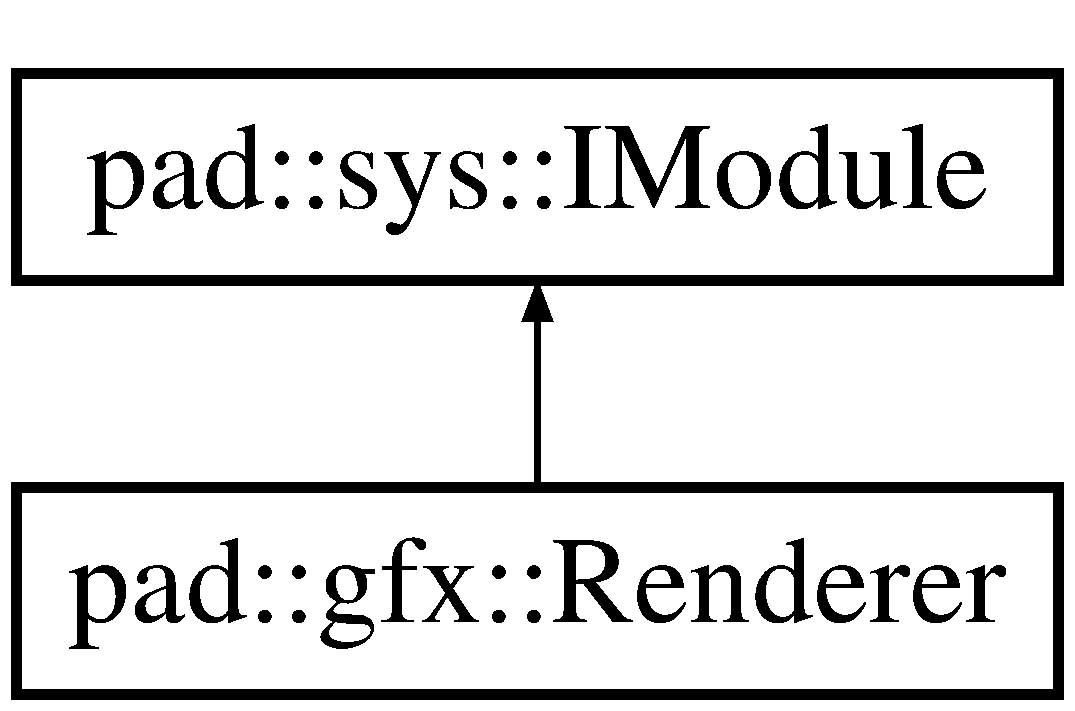
\includegraphics[height=2.000000cm]{classpad_1_1sys_1_1_i_module}
\end{center}
\end{figure}
\subsection*{Public Member Functions}
\begin{DoxyCompactItemize}
\item 
virtual void \mbox{\hyperlink{classpad_1_1sys_1_1_i_module_ad3d5abf3e4d20047b6b64da7db92d1ef}{Start\+Module}} ()=0
\item 
virtual void \mbox{\hyperlink{classpad_1_1sys_1_1_i_module_aa6c2b9d1e6b66aeee291923d4be87f0c}{Stop\+Module}} ()=0
\end{DoxyCompactItemize}


\subsection{Member Function Documentation}
\mbox{\Hypertarget{classpad_1_1sys_1_1_i_module_ad3d5abf3e4d20047b6b64da7db92d1ef}\label{classpad_1_1sys_1_1_i_module_ad3d5abf3e4d20047b6b64da7db92d1ef}} 
\index{pad\+::sys\+::\+I\+Module@{pad\+::sys\+::\+I\+Module}!Start\+Module@{Start\+Module}}
\index{Start\+Module@{Start\+Module}!pad\+::sys\+::\+I\+Module@{pad\+::sys\+::\+I\+Module}}
\subsubsection{\texorpdfstring{Start\+Module()}{StartModule()}}
{\footnotesize\ttfamily virtual void pad\+::sys\+::\+I\+Module\+::\+Start\+Module (\begin{DoxyParamCaption}{ }\end{DoxyParamCaption})\hspace{0.3cm}{\ttfamily [pure virtual]}}



Implemented in \mbox{\hyperlink{classpad_1_1gfx_1_1_renderer_af78164b0fc174776bf1345c99d5c08b4}{pad\+::gfx\+::\+Renderer}}.

\mbox{\Hypertarget{classpad_1_1sys_1_1_i_module_aa6c2b9d1e6b66aeee291923d4be87f0c}\label{classpad_1_1sys_1_1_i_module_aa6c2b9d1e6b66aeee291923d4be87f0c}} 
\index{pad\+::sys\+::\+I\+Module@{pad\+::sys\+::\+I\+Module}!Stop\+Module@{Stop\+Module}}
\index{Stop\+Module@{Stop\+Module}!pad\+::sys\+::\+I\+Module@{pad\+::sys\+::\+I\+Module}}
\subsubsection{\texorpdfstring{Stop\+Module()}{StopModule()}}
{\footnotesize\ttfamily virtual void pad\+::sys\+::\+I\+Module\+::\+Stop\+Module (\begin{DoxyParamCaption}{ }\end{DoxyParamCaption})\hspace{0.3cm}{\ttfamily [pure virtual]}}



Implemented in \mbox{\hyperlink{classpad_1_1gfx_1_1_renderer_ad90dc994132b8f4028eaa5b9af87b601}{pad\+::gfx\+::\+Renderer}}.



The documentation for this class was generated from the following file\+:\begin{DoxyCompactItemize}
\item 
P\+A\+D Engine/\+Sources/\+System/\mbox{\hyperlink{_i_module_8h}{I\+Module.\+h}}\end{DoxyCompactItemize}

\hypertarget{classpad_1_1sys_1_1_i_window_base}{}\section{pad\+:\+:sys\+:\+:I\+Window\+Base Class Reference}
\label{classpad_1_1sys_1_1_i_window_base}\index{pad\+::sys\+::\+I\+Window\+Base@{pad\+::sys\+::\+I\+Window\+Base}}


{\ttfamily \#include $<$I\+Window\+Base.\+h$>$}

Inheritance diagram for pad\+:\+:sys\+:\+:I\+Window\+Base\+:\begin{figure}[H]
\begin{center}
\leavevmode
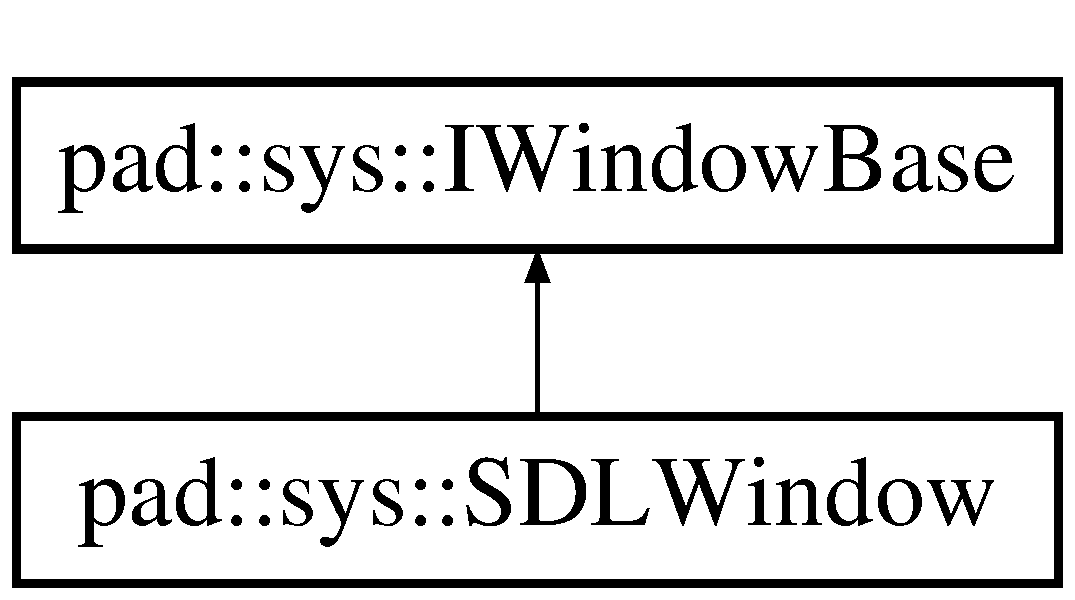
\includegraphics[height=2.000000cm]{classpad_1_1sys_1_1_i_window_base}
\end{center}
\end{figure}
\subsection*{Public Member Functions}
\begin{DoxyCompactItemize}
\item 
virtual void \mbox{\hyperlink{classpad_1_1sys_1_1_i_window_base_aee21db35ea6bdd4299783b4e96a9b326}{Poll\+Events}} ()=0
\item 
virtual void \mbox{\hyperlink{classpad_1_1sys_1_1_i_window_base_a19fff5f21c5a75082d8ca4e2491b269e}{Resize}} (const \mbox{\hyperlink{namespacepad_1_1math_a9773bcf81aa2ddd829bc327d822c6552}{math\+::\+Vec2}}$<$ \mbox{\hyperlink{namespacepad_a03b9241a5f6a191da2faac64714e1038}{uint16}} $>$ \&size)=0
\item 
virtual void \mbox{\hyperlink{classpad_1_1sys_1_1_i_window_base_aff693c784fbf16ae5bbfce797f570879}{Reload\+Settings}} (const \mbox{\hyperlink{structpad_1_1sys_1_1_window_settings}{Window\+Settings}} \&\+\_\+infos)=0
\item 
virtual void \mbox{\hyperlink{classpad_1_1sys_1_1_i_window_base_aee66a6eacff6126f4106a8e725bcbf1f}{Init}} (const \mbox{\hyperlink{structpad_1_1sys_1_1_window_settings}{Window\+Settings}} \&\+\_\+infos)=0
\item 
virtual bool \mbox{\hyperlink{classpad_1_1sys_1_1_i_window_base_a07aae1254b0d8139e912584029d785ea}{Is\+Open}} ()=0
\item 
virtual void \mbox{\hyperlink{classpad_1_1sys_1_1_i_window_base_ac6fe9dea946b20c52ad8d9372e57e6c1}{Swap\+Buffer}} ()=0
\item 
virtual const \mbox{\hyperlink{namespacepad_1_1math_a808a631a6bccd994f9589d7fb86bad41}{math\+::\+Vec2i}} \mbox{\hyperlink{classpad_1_1sys_1_1_i_window_base_ac3cb42c492b8c2ba59f36da4702b7bec}{Get\+Position}} () const =0
\item 
virtual const \mbox{\hyperlink{namespacepad_1_1math_a808a631a6bccd994f9589d7fb86bad41}{math\+::\+Vec2i}} \mbox{\hyperlink{classpad_1_1sys_1_1_i_window_base_acf3540e89da05cc490cf981f196ad771}{Get\+Size}} () const =0
\end{DoxyCompactItemize}
\subsection*{Protected Attributes}
\begin{DoxyCompactItemize}
\item 
bool \mbox{\hyperlink{classpad_1_1sys_1_1_i_window_base_a4ca3e1915cb3c100497ace0d7d04fa23}{m\+\_\+is\+Open}}
\end{DoxyCompactItemize}


\subsection{Member Function Documentation}
\mbox{\Hypertarget{classpad_1_1sys_1_1_i_window_base_ac3cb42c492b8c2ba59f36da4702b7bec}\label{classpad_1_1sys_1_1_i_window_base_ac3cb42c492b8c2ba59f36da4702b7bec}} 
\index{pad\+::sys\+::\+I\+Window\+Base@{pad\+::sys\+::\+I\+Window\+Base}!Get\+Position@{Get\+Position}}
\index{Get\+Position@{Get\+Position}!pad\+::sys\+::\+I\+Window\+Base@{pad\+::sys\+::\+I\+Window\+Base}}
\subsubsection{\texorpdfstring{Get\+Position()}{GetPosition()}}
{\footnotesize\ttfamily virtual const \mbox{\hyperlink{namespacepad_1_1math_a808a631a6bccd994f9589d7fb86bad41}{math\+::\+Vec2i}} pad\+::sys\+::\+I\+Window\+Base\+::\+Get\+Position (\begin{DoxyParamCaption}{ }\end{DoxyParamCaption}) const\hspace{0.3cm}{\ttfamily [pure virtual]}}



Implemented in \mbox{\hyperlink{classpad_1_1sys_1_1_s_d_l_window_a43391052519ec0bc8c194642d6d68d12}{pad\+::sys\+::\+S\+D\+L\+Window}}.

\mbox{\Hypertarget{classpad_1_1sys_1_1_i_window_base_acf3540e89da05cc490cf981f196ad771}\label{classpad_1_1sys_1_1_i_window_base_acf3540e89da05cc490cf981f196ad771}} 
\index{pad\+::sys\+::\+I\+Window\+Base@{pad\+::sys\+::\+I\+Window\+Base}!Get\+Size@{Get\+Size}}
\index{Get\+Size@{Get\+Size}!pad\+::sys\+::\+I\+Window\+Base@{pad\+::sys\+::\+I\+Window\+Base}}
\subsubsection{\texorpdfstring{Get\+Size()}{GetSize()}}
{\footnotesize\ttfamily virtual const \mbox{\hyperlink{namespacepad_1_1math_a808a631a6bccd994f9589d7fb86bad41}{math\+::\+Vec2i}} pad\+::sys\+::\+I\+Window\+Base\+::\+Get\+Size (\begin{DoxyParamCaption}{ }\end{DoxyParamCaption}) const\hspace{0.3cm}{\ttfamily [pure virtual]}}



Implemented in \mbox{\hyperlink{classpad_1_1sys_1_1_s_d_l_window_a4b39d8767776e1fe6f613ad3fe7d7b29}{pad\+::sys\+::\+S\+D\+L\+Window}}.

\mbox{\Hypertarget{classpad_1_1sys_1_1_i_window_base_aee66a6eacff6126f4106a8e725bcbf1f}\label{classpad_1_1sys_1_1_i_window_base_aee66a6eacff6126f4106a8e725bcbf1f}} 
\index{pad\+::sys\+::\+I\+Window\+Base@{pad\+::sys\+::\+I\+Window\+Base}!Init@{Init}}
\index{Init@{Init}!pad\+::sys\+::\+I\+Window\+Base@{pad\+::sys\+::\+I\+Window\+Base}}
\subsubsection{\texorpdfstring{Init()}{Init()}}
{\footnotesize\ttfamily virtual void pad\+::sys\+::\+I\+Window\+Base\+::\+Init (\begin{DoxyParamCaption}\item[{const \mbox{\hyperlink{structpad_1_1sys_1_1_window_settings}{Window\+Settings}} \&}]{\+\_\+infos }\end{DoxyParamCaption})\hspace{0.3cm}{\ttfamily [pure virtual]}}



Implemented in \mbox{\hyperlink{classpad_1_1sys_1_1_s_d_l_window_a7749e49f614ac33a95f1ef4ffed853e7}{pad\+::sys\+::\+S\+D\+L\+Window}}.

\mbox{\Hypertarget{classpad_1_1sys_1_1_i_window_base_a07aae1254b0d8139e912584029d785ea}\label{classpad_1_1sys_1_1_i_window_base_a07aae1254b0d8139e912584029d785ea}} 
\index{pad\+::sys\+::\+I\+Window\+Base@{pad\+::sys\+::\+I\+Window\+Base}!Is\+Open@{Is\+Open}}
\index{Is\+Open@{Is\+Open}!pad\+::sys\+::\+I\+Window\+Base@{pad\+::sys\+::\+I\+Window\+Base}}
\subsubsection{\texorpdfstring{Is\+Open()}{IsOpen()}}
{\footnotesize\ttfamily virtual bool pad\+::sys\+::\+I\+Window\+Base\+::\+Is\+Open (\begin{DoxyParamCaption}{ }\end{DoxyParamCaption})\hspace{0.3cm}{\ttfamily [pure virtual]}}



Implemented in \mbox{\hyperlink{classpad_1_1sys_1_1_s_d_l_window_ae76d9066f3c36e8b949b6c211be0affd}{pad\+::sys\+::\+S\+D\+L\+Window}}.

\mbox{\Hypertarget{classpad_1_1sys_1_1_i_window_base_aee21db35ea6bdd4299783b4e96a9b326}\label{classpad_1_1sys_1_1_i_window_base_aee21db35ea6bdd4299783b4e96a9b326}} 
\index{pad\+::sys\+::\+I\+Window\+Base@{pad\+::sys\+::\+I\+Window\+Base}!Poll\+Events@{Poll\+Events}}
\index{Poll\+Events@{Poll\+Events}!pad\+::sys\+::\+I\+Window\+Base@{pad\+::sys\+::\+I\+Window\+Base}}
\subsubsection{\texorpdfstring{Poll\+Events()}{PollEvents()}}
{\footnotesize\ttfamily virtual void pad\+::sys\+::\+I\+Window\+Base\+::\+Poll\+Events (\begin{DoxyParamCaption}{ }\end{DoxyParamCaption})\hspace{0.3cm}{\ttfamily [pure virtual]}}



Implemented in \mbox{\hyperlink{classpad_1_1sys_1_1_s_d_l_window_a66014e181e30c20a3488ff715d106665}{pad\+::sys\+::\+S\+D\+L\+Window}}.

\mbox{\Hypertarget{classpad_1_1sys_1_1_i_window_base_aff693c784fbf16ae5bbfce797f570879}\label{classpad_1_1sys_1_1_i_window_base_aff693c784fbf16ae5bbfce797f570879}} 
\index{pad\+::sys\+::\+I\+Window\+Base@{pad\+::sys\+::\+I\+Window\+Base}!Reload\+Settings@{Reload\+Settings}}
\index{Reload\+Settings@{Reload\+Settings}!pad\+::sys\+::\+I\+Window\+Base@{pad\+::sys\+::\+I\+Window\+Base}}
\subsubsection{\texorpdfstring{Reload\+Settings()}{ReloadSettings()}}
{\footnotesize\ttfamily virtual void pad\+::sys\+::\+I\+Window\+Base\+::\+Reload\+Settings (\begin{DoxyParamCaption}\item[{const \mbox{\hyperlink{structpad_1_1sys_1_1_window_settings}{Window\+Settings}} \&}]{\+\_\+infos }\end{DoxyParamCaption})\hspace{0.3cm}{\ttfamily [pure virtual]}}



Implemented in \mbox{\hyperlink{classpad_1_1sys_1_1_s_d_l_window_a7f45cd8f1ffa83c4aaedf40b69012870}{pad\+::sys\+::\+S\+D\+L\+Window}}.

\mbox{\Hypertarget{classpad_1_1sys_1_1_i_window_base_a19fff5f21c5a75082d8ca4e2491b269e}\label{classpad_1_1sys_1_1_i_window_base_a19fff5f21c5a75082d8ca4e2491b269e}} 
\index{pad\+::sys\+::\+I\+Window\+Base@{pad\+::sys\+::\+I\+Window\+Base}!Resize@{Resize}}
\index{Resize@{Resize}!pad\+::sys\+::\+I\+Window\+Base@{pad\+::sys\+::\+I\+Window\+Base}}
\subsubsection{\texorpdfstring{Resize()}{Resize()}}
{\footnotesize\ttfamily virtual void pad\+::sys\+::\+I\+Window\+Base\+::\+Resize (\begin{DoxyParamCaption}\item[{const \mbox{\hyperlink{namespacepad_1_1math_a9773bcf81aa2ddd829bc327d822c6552}{math\+::\+Vec2}}$<$ \mbox{\hyperlink{namespacepad_a03b9241a5f6a191da2faac64714e1038}{uint16}} $>$ \&}]{size }\end{DoxyParamCaption})\hspace{0.3cm}{\ttfamily [pure virtual]}}



Implemented in \mbox{\hyperlink{classpad_1_1sys_1_1_s_d_l_window_aba5a51090a6865da6d47826af28413ef}{pad\+::sys\+::\+S\+D\+L\+Window}}.

\mbox{\Hypertarget{classpad_1_1sys_1_1_i_window_base_ac6fe9dea946b20c52ad8d9372e57e6c1}\label{classpad_1_1sys_1_1_i_window_base_ac6fe9dea946b20c52ad8d9372e57e6c1}} 
\index{pad\+::sys\+::\+I\+Window\+Base@{pad\+::sys\+::\+I\+Window\+Base}!Swap\+Buffer@{Swap\+Buffer}}
\index{Swap\+Buffer@{Swap\+Buffer}!pad\+::sys\+::\+I\+Window\+Base@{pad\+::sys\+::\+I\+Window\+Base}}
\subsubsection{\texorpdfstring{Swap\+Buffer()}{SwapBuffer()}}
{\footnotesize\ttfamily virtual void pad\+::sys\+::\+I\+Window\+Base\+::\+Swap\+Buffer (\begin{DoxyParamCaption}{ }\end{DoxyParamCaption})\hspace{0.3cm}{\ttfamily [pure virtual]}}



Implemented in \mbox{\hyperlink{classpad_1_1sys_1_1_s_d_l_window_a991b47b499f3073e4d1962c2512e2ae8}{pad\+::sys\+::\+S\+D\+L\+Window}}.



\subsection{Member Data Documentation}
\mbox{\Hypertarget{classpad_1_1sys_1_1_i_window_base_a4ca3e1915cb3c100497ace0d7d04fa23}\label{classpad_1_1sys_1_1_i_window_base_a4ca3e1915cb3c100497ace0d7d04fa23}} 
\index{pad\+::sys\+::\+I\+Window\+Base@{pad\+::sys\+::\+I\+Window\+Base}!m\+\_\+is\+Open@{m\+\_\+is\+Open}}
\index{m\+\_\+is\+Open@{m\+\_\+is\+Open}!pad\+::sys\+::\+I\+Window\+Base@{pad\+::sys\+::\+I\+Window\+Base}}
\subsubsection{\texorpdfstring{m\+\_\+is\+Open}{m\_isOpen}}
{\footnotesize\ttfamily bool pad\+::sys\+::\+I\+Window\+Base\+::m\+\_\+is\+Open\hspace{0.3cm}{\ttfamily [protected]}}



The documentation for this class was generated from the following file\+:\begin{DoxyCompactItemize}
\item 
P\+A\+D Engine/\+Sources/\+System/\mbox{\hyperlink{_i_window_base_8h}{I\+Window\+Base.\+h}}\end{DoxyCompactItemize}

\hypertarget{structpad_1_1math_1_1_matrix4x4}{}\section{pad\+:\+:math\+:\+:Matrix4x4 Struct Reference}
\label{structpad_1_1math_1_1_matrix4x4}\index{pad\+::math\+::\+Matrix4x4@{pad\+::math\+::\+Matrix4x4}}


{\ttfamily \#include $<$Matrix4x4.\+h$>$}

\subsection*{Public Member Functions}
\begin{DoxyCompactItemize}
\item 
\mbox{\hyperlink{structpad_1_1math_1_1_matrix4x4_a47a4ff74b250afd42a5b31d267de93b2}{Matrix4x4}} ()
\item 
\mbox{\hyperlink{structpad_1_1math_1_1_matrix4x4_aee393ac9af00f6227e7f6d4d6b9f569f}{Matrix4x4}} (float \+\_\+00, float \+\_\+01, float \+\_\+02, float \+\_\+03, float \+\_\+10, float \+\_\+11, float \+\_\+12, float \+\_\+13, float \+\_\+20, float \+\_\+21, float \+\_\+22, float \+\_\+23, float \+\_\+30, float \+\_\+31, float \+\_\+32, float \+\_\+33)
\item 
\mbox{\hyperlink{structpad_1_1math_1_1_matrix4x4_a4765cd7d89d392b63c067353fe2a89f7}{Matrix4x4}} (const float $\ast$\+\_\+data)
\item 
\mbox{\hyperlink{structpad_1_1math_1_1_matrix4x4_a6866f52ee1300609262d13a20ea9a9ad}{Matrix4x4}} (\mbox{\hyperlink{structpad_1_1math_1_1_matrix4x4}{Matrix4x4}} \&\+\_\+matrix)
\item 
\mbox{\hyperlink{structpad_1_1math_1_1_matrix4x4_a2486278c1674f08e20c4d5fbede0b32c}{Matrix4x4}} (\mbox{\hyperlink{structpad_1_1math_1_1_matrix4x4}{Matrix4x4}} \&\&\+\_\+matrix)=default
\item 
\mbox{\hyperlink{structpad_1_1math_1_1_matrix4x4_a19a252dba1b3f4134b0755c8d49ed161}{$\sim$\+Matrix4x4}} ()=default
\item 
float $\ast$ \mbox{\hyperlink{structpad_1_1math_1_1_matrix4x4_acf1ce7bb39d6a1c41db0968d42767b92}{operator\mbox{[}$\,$\mbox{]}}} (const int \+\_\+index)
\item 
void \mbox{\hyperlink{structpad_1_1math_1_1_matrix4x4_ab14377405265dfb8c0adc47974598e7c}{operator=}} (const \mbox{\hyperlink{structpad_1_1math_1_1_matrix4x4}{Matrix4x4}} \&\+\_\+matrix)
\item 
\mbox{\hyperlink{structpad_1_1math_1_1_matrix4x4}{Matrix4x4}} \& \mbox{\hyperlink{structpad_1_1math_1_1_matrix4x4_aab7a3a99bd9ca243483c4a9bdb11243d}{operator=}} (\mbox{\hyperlink{structpad_1_1math_1_1_matrix4x4}{Matrix4x4}} \&\&\+\_\+matrix)=default
\item 
bool \mbox{\hyperlink{structpad_1_1math_1_1_matrix4x4_ae8c88b8c279e8a34a1f3e7e040dc8599}{operator==}} (const \mbox{\hyperlink{structpad_1_1math_1_1_matrix4x4}{Matrix4x4}} \&\+\_\+matrix)
\item 
\mbox{\hyperlink{structpad_1_1math_1_1_matrix4x4}{Matrix4x4}} \mbox{\hyperlink{structpad_1_1math_1_1_matrix4x4_acacb8a40fc9d329f40cdb6f23592e347}{operator+}} (const \mbox{\hyperlink{structpad_1_1math_1_1_matrix4x4}{Matrix4x4}} \&\+\_\+matrix)
\item 
\mbox{\hyperlink{structpad_1_1math_1_1_matrix4x4}{Matrix4x4}} \& \mbox{\hyperlink{structpad_1_1math_1_1_matrix4x4_a41fee92ff1bcaada31a4d5ca828f5486}{operator+=}} (const \mbox{\hyperlink{structpad_1_1math_1_1_matrix4x4}{Matrix4x4}} \&\+\_\+matrix)
\item 
\mbox{\hyperlink{structpad_1_1math_1_1_matrix4x4}{Matrix4x4}} \mbox{\hyperlink{structpad_1_1math_1_1_matrix4x4_a15e852769583fe62d7691a9f55b15d2f}{operator-\/}} (const \mbox{\hyperlink{structpad_1_1math_1_1_matrix4x4}{Matrix4x4}} \&\+\_\+matrix)
\item 
\mbox{\hyperlink{structpad_1_1math_1_1_matrix4x4}{Matrix4x4}} \& \mbox{\hyperlink{structpad_1_1math_1_1_matrix4x4_a9ff7cd4357169ae04f5330dfa1a3bb64}{operator-\/=}} (const \mbox{\hyperlink{structpad_1_1math_1_1_matrix4x4}{Matrix4x4}} \&\+\_\+matrix)
\item 
\mbox{\hyperlink{structpad_1_1math_1_1_matrix4x4}{Matrix4x4}} \mbox{\hyperlink{structpad_1_1math_1_1_matrix4x4_a6f3bc37ce2fcfa89fa7b9e641969e684}{operator$\ast$}} (const \mbox{\hyperlink{structpad_1_1math_1_1_matrix4x4}{Matrix4x4}} \&\+\_\+matrix)
\item 
\mbox{\hyperlink{structpad_1_1math_1_1_matrix4x4}{Matrix4x4}} \& \mbox{\hyperlink{structpad_1_1math_1_1_matrix4x4_a78d1c63256e91dcd87fe34f3e1f42246}{operator$\ast$=}} (const \mbox{\hyperlink{structpad_1_1math_1_1_matrix4x4}{Matrix4x4}} \&\+\_\+matrix)
\end{DoxyCompactItemize}
\subsection*{Public Attributes}
\begin{DoxyCompactItemize}
\item 
\begin{tabbing}
xx\=xx\=xx\=xx\=xx\=xx\=xx\=xx\=xx\=\kill
union \{\\
\>float \mbox{\hyperlink{structpad_1_1math_1_1_matrix4x4_a3ce7e8b8246a13268d4bc9c5d2f202f7}{data}} \mbox{[}16\mbox{]}\\
\>\_\_m256 \mbox{\hyperlink{structpad_1_1math_1_1_matrix4x4_a1943e1b4a06834d2ff79192b9688463c}{\_\_DATA256}} \mbox{[}2\mbox{]}\\
\>\_\_m128 \mbox{\hyperlink{structpad_1_1math_1_1_matrix4x4_ac736c31530295349e0ba6a0cfa566271}{\_\_DATA128}} \mbox{[}4\mbox{]}\\
\}; \\

\end{tabbing}\end{DoxyCompactItemize}


\subsection{Constructor \& Destructor Documentation}
\mbox{\Hypertarget{structpad_1_1math_1_1_matrix4x4_a47a4ff74b250afd42a5b31d267de93b2}\label{structpad_1_1math_1_1_matrix4x4_a47a4ff74b250afd42a5b31d267de93b2}} 
\index{pad\+::math\+::\+Matrix4x4@{pad\+::math\+::\+Matrix4x4}!Matrix4x4@{Matrix4x4}}
\index{Matrix4x4@{Matrix4x4}!pad\+::math\+::\+Matrix4x4@{pad\+::math\+::\+Matrix4x4}}
\subsubsection{\texorpdfstring{Matrix4x4()}{Matrix4x4()}\hspace{0.1cm}{\footnotesize\ttfamily [1/5]}}
{\footnotesize\ttfamily pad\+::math\+::\+Matrix4x4\+::\+Matrix4x4 (\begin{DoxyParamCaption}{ }\end{DoxyParamCaption})}

\mbox{\Hypertarget{structpad_1_1math_1_1_matrix4x4_aee393ac9af00f6227e7f6d4d6b9f569f}\label{structpad_1_1math_1_1_matrix4x4_aee393ac9af00f6227e7f6d4d6b9f569f}} 
\index{pad\+::math\+::\+Matrix4x4@{pad\+::math\+::\+Matrix4x4}!Matrix4x4@{Matrix4x4}}
\index{Matrix4x4@{Matrix4x4}!pad\+::math\+::\+Matrix4x4@{pad\+::math\+::\+Matrix4x4}}
\subsubsection{\texorpdfstring{Matrix4x4()}{Matrix4x4()}\hspace{0.1cm}{\footnotesize\ttfamily [2/5]}}
{\footnotesize\ttfamily pad\+::math\+::\+Matrix4x4\+::\+Matrix4x4 (\begin{DoxyParamCaption}\item[{float}]{\+\_\+00,  }\item[{float}]{\+\_\+01,  }\item[{float}]{\+\_\+02,  }\item[{float}]{\+\_\+03,  }\item[{float}]{\+\_\+10,  }\item[{float}]{\+\_\+11,  }\item[{float}]{\+\_\+12,  }\item[{float}]{\+\_\+13,  }\item[{float}]{\+\_\+20,  }\item[{float}]{\+\_\+21,  }\item[{float}]{\+\_\+22,  }\item[{float}]{\+\_\+23,  }\item[{float}]{\+\_\+30,  }\item[{float}]{\+\_\+31,  }\item[{float}]{\+\_\+32,  }\item[{float}]{\+\_\+33 }\end{DoxyParamCaption})}

\mbox{\Hypertarget{structpad_1_1math_1_1_matrix4x4_a4765cd7d89d392b63c067353fe2a89f7}\label{structpad_1_1math_1_1_matrix4x4_a4765cd7d89d392b63c067353fe2a89f7}} 
\index{pad\+::math\+::\+Matrix4x4@{pad\+::math\+::\+Matrix4x4}!Matrix4x4@{Matrix4x4}}
\index{Matrix4x4@{Matrix4x4}!pad\+::math\+::\+Matrix4x4@{pad\+::math\+::\+Matrix4x4}}
\subsubsection{\texorpdfstring{Matrix4x4()}{Matrix4x4()}\hspace{0.1cm}{\footnotesize\ttfamily [3/5]}}
{\footnotesize\ttfamily pad\+::math\+::\+Matrix4x4\+::\+Matrix4x4 (\begin{DoxyParamCaption}\item[{const float $\ast$}]{\+\_\+data }\end{DoxyParamCaption})}

\mbox{\Hypertarget{structpad_1_1math_1_1_matrix4x4_a6866f52ee1300609262d13a20ea9a9ad}\label{structpad_1_1math_1_1_matrix4x4_a6866f52ee1300609262d13a20ea9a9ad}} 
\index{pad\+::math\+::\+Matrix4x4@{pad\+::math\+::\+Matrix4x4}!Matrix4x4@{Matrix4x4}}
\index{Matrix4x4@{Matrix4x4}!pad\+::math\+::\+Matrix4x4@{pad\+::math\+::\+Matrix4x4}}
\subsubsection{\texorpdfstring{Matrix4x4()}{Matrix4x4()}\hspace{0.1cm}{\footnotesize\ttfamily [4/5]}}
{\footnotesize\ttfamily pad\+::math\+::\+Matrix4x4\+::\+Matrix4x4 (\begin{DoxyParamCaption}\item[{\mbox{\hyperlink{structpad_1_1math_1_1_matrix4x4}{Matrix4x4}} \&}]{\+\_\+matrix }\end{DoxyParamCaption})}

\mbox{\Hypertarget{structpad_1_1math_1_1_matrix4x4_a2486278c1674f08e20c4d5fbede0b32c}\label{structpad_1_1math_1_1_matrix4x4_a2486278c1674f08e20c4d5fbede0b32c}} 
\index{pad\+::math\+::\+Matrix4x4@{pad\+::math\+::\+Matrix4x4}!Matrix4x4@{Matrix4x4}}
\index{Matrix4x4@{Matrix4x4}!pad\+::math\+::\+Matrix4x4@{pad\+::math\+::\+Matrix4x4}}
\subsubsection{\texorpdfstring{Matrix4x4()}{Matrix4x4()}\hspace{0.1cm}{\footnotesize\ttfamily [5/5]}}
{\footnotesize\ttfamily pad\+::math\+::\+Matrix4x4\+::\+Matrix4x4 (\begin{DoxyParamCaption}\item[{\mbox{\hyperlink{structpad_1_1math_1_1_matrix4x4}{Matrix4x4}} \&\&}]{\+\_\+matrix }\end{DoxyParamCaption})\hspace{0.3cm}{\ttfamily [default]}}

\mbox{\Hypertarget{structpad_1_1math_1_1_matrix4x4_a19a252dba1b3f4134b0755c8d49ed161}\label{structpad_1_1math_1_1_matrix4x4_a19a252dba1b3f4134b0755c8d49ed161}} 
\index{pad\+::math\+::\+Matrix4x4@{pad\+::math\+::\+Matrix4x4}!````~Matrix4x4@{$\sim$\+Matrix4x4}}
\index{````~Matrix4x4@{$\sim$\+Matrix4x4}!pad\+::math\+::\+Matrix4x4@{pad\+::math\+::\+Matrix4x4}}
\subsubsection{\texorpdfstring{$\sim$\+Matrix4x4()}{~Matrix4x4()}}
{\footnotesize\ttfamily pad\+::math\+::\+Matrix4x4\+::$\sim$\+Matrix4x4 (\begin{DoxyParamCaption}{ }\end{DoxyParamCaption})\hspace{0.3cm}{\ttfamily [default]}}



\subsection{Member Function Documentation}
\mbox{\Hypertarget{structpad_1_1math_1_1_matrix4x4_a6f3bc37ce2fcfa89fa7b9e641969e684}\label{structpad_1_1math_1_1_matrix4x4_a6f3bc37ce2fcfa89fa7b9e641969e684}} 
\index{pad\+::math\+::\+Matrix4x4@{pad\+::math\+::\+Matrix4x4}!operator$\ast$@{operator$\ast$}}
\index{operator$\ast$@{operator$\ast$}!pad\+::math\+::\+Matrix4x4@{pad\+::math\+::\+Matrix4x4}}
\subsubsection{\texorpdfstring{operator$\ast$()}{operator*()}}
{\footnotesize\ttfamily \mbox{\hyperlink{structpad_1_1math_1_1_matrix4x4}{Matrix4x4}} pad\+::math\+::\+Matrix4x4\+::operator$\ast$ (\begin{DoxyParamCaption}\item[{const \mbox{\hyperlink{structpad_1_1math_1_1_matrix4x4}{Matrix4x4}} \&}]{\+\_\+matrix }\end{DoxyParamCaption})}

\mbox{\Hypertarget{structpad_1_1math_1_1_matrix4x4_a78d1c63256e91dcd87fe34f3e1f42246}\label{structpad_1_1math_1_1_matrix4x4_a78d1c63256e91dcd87fe34f3e1f42246}} 
\index{pad\+::math\+::\+Matrix4x4@{pad\+::math\+::\+Matrix4x4}!operator$\ast$=@{operator$\ast$=}}
\index{operator$\ast$=@{operator$\ast$=}!pad\+::math\+::\+Matrix4x4@{pad\+::math\+::\+Matrix4x4}}
\subsubsection{\texorpdfstring{operator$\ast$=()}{operator*=()}}
{\footnotesize\ttfamily \mbox{\hyperlink{structpad_1_1math_1_1_matrix4x4}{Matrix4x4}} \& pad\+::math\+::\+Matrix4x4\+::operator$\ast$= (\begin{DoxyParamCaption}\item[{const \mbox{\hyperlink{structpad_1_1math_1_1_matrix4x4}{Matrix4x4}} \&}]{\+\_\+matrix }\end{DoxyParamCaption})}

\mbox{\Hypertarget{structpad_1_1math_1_1_matrix4x4_acacb8a40fc9d329f40cdb6f23592e347}\label{structpad_1_1math_1_1_matrix4x4_acacb8a40fc9d329f40cdb6f23592e347}} 
\index{pad\+::math\+::\+Matrix4x4@{pad\+::math\+::\+Matrix4x4}!operator+@{operator+}}
\index{operator+@{operator+}!pad\+::math\+::\+Matrix4x4@{pad\+::math\+::\+Matrix4x4}}
\subsubsection{\texorpdfstring{operator+()}{operator+()}}
{\footnotesize\ttfamily \mbox{\hyperlink{structpad_1_1math_1_1_matrix4x4}{Matrix4x4}} pad\+::math\+::\+Matrix4x4\+::operator+ (\begin{DoxyParamCaption}\item[{const \mbox{\hyperlink{structpad_1_1math_1_1_matrix4x4}{Matrix4x4}} \&}]{\+\_\+matrix }\end{DoxyParamCaption})}

\mbox{\Hypertarget{structpad_1_1math_1_1_matrix4x4_a41fee92ff1bcaada31a4d5ca828f5486}\label{structpad_1_1math_1_1_matrix4x4_a41fee92ff1bcaada31a4d5ca828f5486}} 
\index{pad\+::math\+::\+Matrix4x4@{pad\+::math\+::\+Matrix4x4}!operator+=@{operator+=}}
\index{operator+=@{operator+=}!pad\+::math\+::\+Matrix4x4@{pad\+::math\+::\+Matrix4x4}}
\subsubsection{\texorpdfstring{operator+=()}{operator+=()}}
{\footnotesize\ttfamily \mbox{\hyperlink{structpad_1_1math_1_1_matrix4x4}{Matrix4x4}} \& pad\+::math\+::\+Matrix4x4\+::operator+= (\begin{DoxyParamCaption}\item[{const \mbox{\hyperlink{structpad_1_1math_1_1_matrix4x4}{Matrix4x4}} \&}]{\+\_\+matrix }\end{DoxyParamCaption})}

\mbox{\Hypertarget{structpad_1_1math_1_1_matrix4x4_a15e852769583fe62d7691a9f55b15d2f}\label{structpad_1_1math_1_1_matrix4x4_a15e852769583fe62d7691a9f55b15d2f}} 
\index{pad\+::math\+::\+Matrix4x4@{pad\+::math\+::\+Matrix4x4}!operator-\/@{operator-\/}}
\index{operator-\/@{operator-\/}!pad\+::math\+::\+Matrix4x4@{pad\+::math\+::\+Matrix4x4}}
\subsubsection{\texorpdfstring{operator-\/()}{operator-()}}
{\footnotesize\ttfamily \mbox{\hyperlink{structpad_1_1math_1_1_matrix4x4}{Matrix4x4}} pad\+::math\+::\+Matrix4x4\+::operator-\/ (\begin{DoxyParamCaption}\item[{const \mbox{\hyperlink{structpad_1_1math_1_1_matrix4x4}{Matrix4x4}} \&}]{\+\_\+matrix }\end{DoxyParamCaption})}

\mbox{\Hypertarget{structpad_1_1math_1_1_matrix4x4_a9ff7cd4357169ae04f5330dfa1a3bb64}\label{structpad_1_1math_1_1_matrix4x4_a9ff7cd4357169ae04f5330dfa1a3bb64}} 
\index{pad\+::math\+::\+Matrix4x4@{pad\+::math\+::\+Matrix4x4}!operator-\/=@{operator-\/=}}
\index{operator-\/=@{operator-\/=}!pad\+::math\+::\+Matrix4x4@{pad\+::math\+::\+Matrix4x4}}
\subsubsection{\texorpdfstring{operator-\/=()}{operator-=()}}
{\footnotesize\ttfamily \mbox{\hyperlink{structpad_1_1math_1_1_matrix4x4}{Matrix4x4}} \& pad\+::math\+::\+Matrix4x4\+::operator-\/= (\begin{DoxyParamCaption}\item[{const \mbox{\hyperlink{structpad_1_1math_1_1_matrix4x4}{Matrix4x4}} \&}]{\+\_\+matrix }\end{DoxyParamCaption})}

\mbox{\Hypertarget{structpad_1_1math_1_1_matrix4x4_ab14377405265dfb8c0adc47974598e7c}\label{structpad_1_1math_1_1_matrix4x4_ab14377405265dfb8c0adc47974598e7c}} 
\index{pad\+::math\+::\+Matrix4x4@{pad\+::math\+::\+Matrix4x4}!operator=@{operator=}}
\index{operator=@{operator=}!pad\+::math\+::\+Matrix4x4@{pad\+::math\+::\+Matrix4x4}}
\subsubsection{\texorpdfstring{operator=()}{operator=()}\hspace{0.1cm}{\footnotesize\ttfamily [1/2]}}
{\footnotesize\ttfamily void pad\+::math\+::\+Matrix4x4\+::operator= (\begin{DoxyParamCaption}\item[{const \mbox{\hyperlink{structpad_1_1math_1_1_matrix4x4}{Matrix4x4}} \&}]{\+\_\+matrix }\end{DoxyParamCaption})}

\mbox{\Hypertarget{structpad_1_1math_1_1_matrix4x4_aab7a3a99bd9ca243483c4a9bdb11243d}\label{structpad_1_1math_1_1_matrix4x4_aab7a3a99bd9ca243483c4a9bdb11243d}} 
\index{pad\+::math\+::\+Matrix4x4@{pad\+::math\+::\+Matrix4x4}!operator=@{operator=}}
\index{operator=@{operator=}!pad\+::math\+::\+Matrix4x4@{pad\+::math\+::\+Matrix4x4}}
\subsubsection{\texorpdfstring{operator=()}{operator=()}\hspace{0.1cm}{\footnotesize\ttfamily [2/2]}}
{\footnotesize\ttfamily \mbox{\hyperlink{structpad_1_1math_1_1_matrix4x4}{Matrix4x4}}\& pad\+::math\+::\+Matrix4x4\+::operator= (\begin{DoxyParamCaption}\item[{\mbox{\hyperlink{structpad_1_1math_1_1_matrix4x4}{Matrix4x4}} \&\&}]{\+\_\+matrix }\end{DoxyParamCaption})\hspace{0.3cm}{\ttfamily [default]}}

\mbox{\Hypertarget{structpad_1_1math_1_1_matrix4x4_ae8c88b8c279e8a34a1f3e7e040dc8599}\label{structpad_1_1math_1_1_matrix4x4_ae8c88b8c279e8a34a1f3e7e040dc8599}} 
\index{pad\+::math\+::\+Matrix4x4@{pad\+::math\+::\+Matrix4x4}!operator==@{operator==}}
\index{operator==@{operator==}!pad\+::math\+::\+Matrix4x4@{pad\+::math\+::\+Matrix4x4}}
\subsubsection{\texorpdfstring{operator==()}{operator==()}}
{\footnotesize\ttfamily bool pad\+::math\+::\+Matrix4x4\+::operator== (\begin{DoxyParamCaption}\item[{const \mbox{\hyperlink{structpad_1_1math_1_1_matrix4x4}{Matrix4x4}} \&}]{\+\_\+matrix }\end{DoxyParamCaption})}

\mbox{\Hypertarget{structpad_1_1math_1_1_matrix4x4_acf1ce7bb39d6a1c41db0968d42767b92}\label{structpad_1_1math_1_1_matrix4x4_acf1ce7bb39d6a1c41db0968d42767b92}} 
\index{pad\+::math\+::\+Matrix4x4@{pad\+::math\+::\+Matrix4x4}!operator\mbox{[}\mbox{]}@{operator[]}}
\index{operator\mbox{[}\mbox{]}@{operator[]}!pad\+::math\+::\+Matrix4x4@{pad\+::math\+::\+Matrix4x4}}
\subsubsection{\texorpdfstring{operator[]()}{operator[]()}}
{\footnotesize\ttfamily float $\ast$ pad\+::math\+::\+Matrix4x4\+::operator\mbox{[}$\,$\mbox{]} (\begin{DoxyParamCaption}\item[{const int}]{\+\_\+index }\end{DoxyParamCaption})}



\subsection{Member Data Documentation}
\mbox{\Hypertarget{structpad_1_1math_1_1_matrix4x4_a161495713e9e144c1990df8faff47e98}\label{structpad_1_1math_1_1_matrix4x4_a161495713e9e144c1990df8faff47e98}} 
\subsubsection{\texorpdfstring{"@1}{@1}}
{\footnotesize\ttfamily union \{ ... \} }

\mbox{\Hypertarget{structpad_1_1math_1_1_matrix4x4_ac736c31530295349e0ba6a0cfa566271}\label{structpad_1_1math_1_1_matrix4x4_ac736c31530295349e0ba6a0cfa566271}} 
\index{pad\+::math\+::\+Matrix4x4@{pad\+::math\+::\+Matrix4x4}!\+\_\+\+\_\+\+D\+A\+T\+A128@{\+\_\+\+\_\+\+D\+A\+T\+A128}}
\index{\+\_\+\+\_\+\+D\+A\+T\+A128@{\+\_\+\+\_\+\+D\+A\+T\+A128}!pad\+::math\+::\+Matrix4x4@{pad\+::math\+::\+Matrix4x4}}
\subsubsection{\texorpdfstring{\+\_\+\+\_\+\+D\+A\+T\+A128}{\_\_DATA128}}
{\footnotesize\ttfamily \+\_\+\+\_\+m128 pad\+::math\+::\+Matrix4x4\+::\+\_\+\+\_\+\+D\+A\+T\+A128\mbox{[}4\mbox{]}}

\mbox{\Hypertarget{structpad_1_1math_1_1_matrix4x4_a1943e1b4a06834d2ff79192b9688463c}\label{structpad_1_1math_1_1_matrix4x4_a1943e1b4a06834d2ff79192b9688463c}} 
\index{pad\+::math\+::\+Matrix4x4@{pad\+::math\+::\+Matrix4x4}!\+\_\+\+\_\+\+D\+A\+T\+A256@{\+\_\+\+\_\+\+D\+A\+T\+A256}}
\index{\+\_\+\+\_\+\+D\+A\+T\+A256@{\+\_\+\+\_\+\+D\+A\+T\+A256}!pad\+::math\+::\+Matrix4x4@{pad\+::math\+::\+Matrix4x4}}
\subsubsection{\texorpdfstring{\+\_\+\+\_\+\+D\+A\+T\+A256}{\_\_DATA256}}
{\footnotesize\ttfamily \+\_\+\+\_\+m256 pad\+::math\+::\+Matrix4x4\+::\+\_\+\+\_\+\+D\+A\+T\+A256\mbox{[}2\mbox{]}}

\mbox{\Hypertarget{structpad_1_1math_1_1_matrix4x4_a3ce7e8b8246a13268d4bc9c5d2f202f7}\label{structpad_1_1math_1_1_matrix4x4_a3ce7e8b8246a13268d4bc9c5d2f202f7}} 
\index{pad\+::math\+::\+Matrix4x4@{pad\+::math\+::\+Matrix4x4}!data@{data}}
\index{data@{data}!pad\+::math\+::\+Matrix4x4@{pad\+::math\+::\+Matrix4x4}}
\subsubsection{\texorpdfstring{data}{data}}
{\footnotesize\ttfamily float pad\+::math\+::\+Matrix4x4\+::data\mbox{[}16\mbox{]}}



The documentation for this struct was generated from the following files\+:\begin{DoxyCompactItemize}
\item 
Math/\+Sources/\+Math/\mbox{\hyperlink{_matrix4x4_8h}{Matrix4x4.\+h}}\item 
Math/\+Sources/\+Math/\mbox{\hyperlink{_matrix4x4__impl_8h}{Matrix4x4\+\_\+impl.\+h}}\end{DoxyCompactItemize}

\hypertarget{classpad_1_1gfx_1_1_renderer}{}\section{pad\+:\+:gfx\+:\+:Renderer Class Reference}
\label{classpad_1_1gfx_1_1_renderer}\index{pad\+::gfx\+::\+Renderer@{pad\+::gfx\+::\+Renderer}}


{\ttfamily \#include $<$Renderer.\+h$>$}

Inheritance diagram for pad\+:\+:gfx\+:\+:Renderer\+:\begin{figure}[H]
\begin{center}
\leavevmode
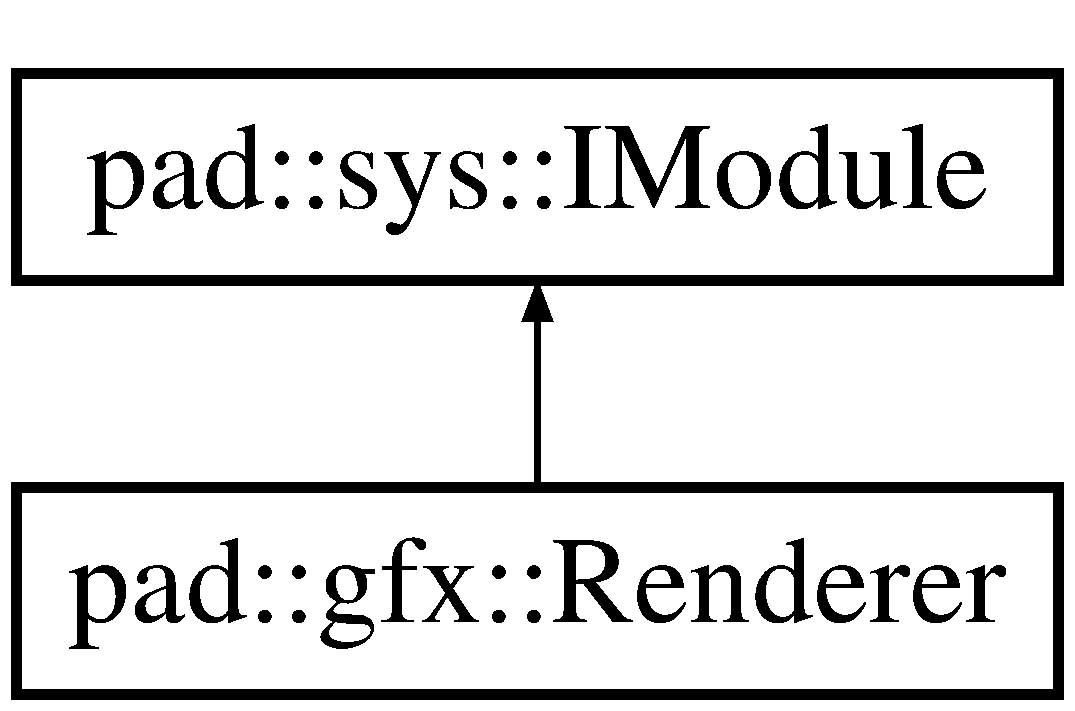
\includegraphics[height=2.000000cm]{classpad_1_1gfx_1_1_renderer}
\end{center}
\end{figure}
\subsection*{Public Member Functions}
\begin{DoxyCompactItemize}
\item 
\mbox{\hyperlink{classpad_1_1gfx_1_1_renderer_a31e4f7095746776998b8d9826dd48e69}{Renderer}} ()
\item 
virtual \mbox{\hyperlink{classpad_1_1gfx_1_1_renderer_a104d47988f127a95e78ed01a29b70d39}{$\sim$\+Renderer}} ()=default
\item 
\mbox{\hyperlink{classpad_1_1gfx_1_1_renderer_a2bcf737a8d0e8964e69aa391995335d2}{Renderer}} (const \mbox{\hyperlink{classpad_1_1gfx_1_1_renderer}{Renderer}} \&)=delete
\item 
\mbox{\hyperlink{classpad_1_1gfx_1_1_renderer_afef3c09f0e69578c3c70a271d37b5c86}{Renderer}} (\mbox{\hyperlink{classpad_1_1gfx_1_1_renderer}{Renderer}} \&\&)=delete
\item 
virtual void \mbox{\hyperlink{classpad_1_1gfx_1_1_renderer_af78164b0fc174776bf1345c99d5c08b4}{Start\+Module}} ()
\item 
virtual void \mbox{\hyperlink{classpad_1_1gfx_1_1_renderer_ad90dc994132b8f4028eaa5b9af87b601}{Stop\+Module}} ()
\item 
void \mbox{\hyperlink{classpad_1_1gfx_1_1_renderer_a28ca09b90cf50729dcca9e6c6e7150d3}{Init}} (const \mbox{\hyperlink{structpad_1_1gfx_1_1_render_settings}{Render\+Settings}} \&settings)
\item 
void \mbox{\hyperlink{classpad_1_1gfx_1_1_renderer_a9a2be08d5d678ba36dbf94f2690c57fb}{Clear\+Buffer}} ()
\item 
void \mbox{\hyperlink{classpad_1_1gfx_1_1_renderer_ae7e6d57e172a8921b44fe41e976f0d0f}{Draw}} ()
\item 
void \mbox{\hyperlink{classpad_1_1gfx_1_1_renderer_a0988ec219668aa3a4410c31161cac8ac}{operator=}} (const \mbox{\hyperlink{classpad_1_1gfx_1_1_renderer}{Renderer}} \&)=delete
\item 
void \mbox{\hyperlink{classpad_1_1gfx_1_1_renderer_a2ea30dd98eda5c1a840d598e8de57dc1}{operator=}} (\mbox{\hyperlink{classpad_1_1gfx_1_1_renderer}{Renderer}} \&\&)=delete
\end{DoxyCompactItemize}
\subsection*{Private Member Functions}
\begin{DoxyCompactItemize}
\item 
void \mbox{\hyperlink{classpad_1_1gfx_1_1_renderer_a231a9121b1b95e52eae5fab21cd8785c}{Init\+Context}} (const \mbox{\hyperlink{namespacepad_1_1math_a4eb77014ac7b74bd24cf73bca82ac3a3}{math\+::\+Vec4f}} \&\+\_\+clear\+Color)
\item 
void \mbox{\hyperlink{classpad_1_1gfx_1_1_renderer_a403e00bd5a3c5f91c5505332dda41a3e}{Init\+View\+Port}} (const \mbox{\hyperlink{namespacepad_1_1math_a808a631a6bccd994f9589d7fb86bad41}{math\+::\+Vec2i}} \&\+\_\+viewport\+Size)
\end{DoxyCompactItemize}


\subsection{Constructor \& Destructor Documentation}
\mbox{\Hypertarget{classpad_1_1gfx_1_1_renderer_a31e4f7095746776998b8d9826dd48e69}\label{classpad_1_1gfx_1_1_renderer_a31e4f7095746776998b8d9826dd48e69}} 
\index{pad\+::gfx\+::\+Renderer@{pad\+::gfx\+::\+Renderer}!Renderer@{Renderer}}
\index{Renderer@{Renderer}!pad\+::gfx\+::\+Renderer@{pad\+::gfx\+::\+Renderer}}
\subsubsection{\texorpdfstring{Renderer()}{Renderer()}\hspace{0.1cm}{\footnotesize\ttfamily [1/3]}}
{\footnotesize\ttfamily pad\+::gfx\+::\+Renderer\+::\+Renderer (\begin{DoxyParamCaption}{ }\end{DoxyParamCaption})}

\mbox{\Hypertarget{classpad_1_1gfx_1_1_renderer_a104d47988f127a95e78ed01a29b70d39}\label{classpad_1_1gfx_1_1_renderer_a104d47988f127a95e78ed01a29b70d39}} 
\index{pad\+::gfx\+::\+Renderer@{pad\+::gfx\+::\+Renderer}!````~Renderer@{$\sim$\+Renderer}}
\index{````~Renderer@{$\sim$\+Renderer}!pad\+::gfx\+::\+Renderer@{pad\+::gfx\+::\+Renderer}}
\subsubsection{\texorpdfstring{$\sim$\+Renderer()}{~Renderer()}}
{\footnotesize\ttfamily virtual pad\+::gfx\+::\+Renderer\+::$\sim$\+Renderer (\begin{DoxyParamCaption}{ }\end{DoxyParamCaption})\hspace{0.3cm}{\ttfamily [virtual]}, {\ttfamily [default]}}

\mbox{\Hypertarget{classpad_1_1gfx_1_1_renderer_a2bcf737a8d0e8964e69aa391995335d2}\label{classpad_1_1gfx_1_1_renderer_a2bcf737a8d0e8964e69aa391995335d2}} 
\index{pad\+::gfx\+::\+Renderer@{pad\+::gfx\+::\+Renderer}!Renderer@{Renderer}}
\index{Renderer@{Renderer}!pad\+::gfx\+::\+Renderer@{pad\+::gfx\+::\+Renderer}}
\subsubsection{\texorpdfstring{Renderer()}{Renderer()}\hspace{0.1cm}{\footnotesize\ttfamily [2/3]}}
{\footnotesize\ttfamily pad\+::gfx\+::\+Renderer\+::\+Renderer (\begin{DoxyParamCaption}\item[{const \mbox{\hyperlink{classpad_1_1gfx_1_1_renderer}{Renderer}} \&}]{ }\end{DoxyParamCaption})\hspace{0.3cm}{\ttfamily [delete]}}

\mbox{\Hypertarget{classpad_1_1gfx_1_1_renderer_afef3c09f0e69578c3c70a271d37b5c86}\label{classpad_1_1gfx_1_1_renderer_afef3c09f0e69578c3c70a271d37b5c86}} 
\index{pad\+::gfx\+::\+Renderer@{pad\+::gfx\+::\+Renderer}!Renderer@{Renderer}}
\index{Renderer@{Renderer}!pad\+::gfx\+::\+Renderer@{pad\+::gfx\+::\+Renderer}}
\subsubsection{\texorpdfstring{Renderer()}{Renderer()}\hspace{0.1cm}{\footnotesize\ttfamily [3/3]}}
{\footnotesize\ttfamily pad\+::gfx\+::\+Renderer\+::\+Renderer (\begin{DoxyParamCaption}\item[{\mbox{\hyperlink{classpad_1_1gfx_1_1_renderer}{Renderer}} \&\&}]{ }\end{DoxyParamCaption})\hspace{0.3cm}{\ttfamily [delete]}}



\subsection{Member Function Documentation}
\mbox{\Hypertarget{classpad_1_1gfx_1_1_renderer_a9a2be08d5d678ba36dbf94f2690c57fb}\label{classpad_1_1gfx_1_1_renderer_a9a2be08d5d678ba36dbf94f2690c57fb}} 
\index{pad\+::gfx\+::\+Renderer@{pad\+::gfx\+::\+Renderer}!Clear\+Buffer@{Clear\+Buffer}}
\index{Clear\+Buffer@{Clear\+Buffer}!pad\+::gfx\+::\+Renderer@{pad\+::gfx\+::\+Renderer}}
\subsubsection{\texorpdfstring{Clear\+Buffer()}{ClearBuffer()}}
{\footnotesize\ttfamily void pad\+::gfx\+::\+Renderer\+::\+Clear\+Buffer (\begin{DoxyParamCaption}{ }\end{DoxyParamCaption})}

\mbox{\Hypertarget{classpad_1_1gfx_1_1_renderer_ae7e6d57e172a8921b44fe41e976f0d0f}\label{classpad_1_1gfx_1_1_renderer_ae7e6d57e172a8921b44fe41e976f0d0f}} 
\index{pad\+::gfx\+::\+Renderer@{pad\+::gfx\+::\+Renderer}!Draw@{Draw}}
\index{Draw@{Draw}!pad\+::gfx\+::\+Renderer@{pad\+::gfx\+::\+Renderer}}
\subsubsection{\texorpdfstring{Draw()}{Draw()}}
{\footnotesize\ttfamily void pad\+::gfx\+::\+Renderer\+::\+Draw (\begin{DoxyParamCaption}{ }\end{DoxyParamCaption})}

\mbox{\Hypertarget{classpad_1_1gfx_1_1_renderer_a28ca09b90cf50729dcca9e6c6e7150d3}\label{classpad_1_1gfx_1_1_renderer_a28ca09b90cf50729dcca9e6c6e7150d3}} 
\index{pad\+::gfx\+::\+Renderer@{pad\+::gfx\+::\+Renderer}!Init@{Init}}
\index{Init@{Init}!pad\+::gfx\+::\+Renderer@{pad\+::gfx\+::\+Renderer}}
\subsubsection{\texorpdfstring{Init()}{Init()}}
{\footnotesize\ttfamily void pad\+::gfx\+::\+Renderer\+::\+Init (\begin{DoxyParamCaption}\item[{const \mbox{\hyperlink{structpad_1_1gfx_1_1_render_settings}{Render\+Settings}} \&}]{settings }\end{DoxyParamCaption})}

\mbox{\Hypertarget{classpad_1_1gfx_1_1_renderer_a231a9121b1b95e52eae5fab21cd8785c}\label{classpad_1_1gfx_1_1_renderer_a231a9121b1b95e52eae5fab21cd8785c}} 
\index{pad\+::gfx\+::\+Renderer@{pad\+::gfx\+::\+Renderer}!Init\+Context@{Init\+Context}}
\index{Init\+Context@{Init\+Context}!pad\+::gfx\+::\+Renderer@{pad\+::gfx\+::\+Renderer}}
\subsubsection{\texorpdfstring{Init\+Context()}{InitContext()}}
{\footnotesize\ttfamily void pad\+::gfx\+::\+Renderer\+::\+Init\+Context (\begin{DoxyParamCaption}\item[{const \mbox{\hyperlink{namespacepad_1_1math_a4eb77014ac7b74bd24cf73bca82ac3a3}{math\+::\+Vec4f}} \&}]{\+\_\+clear\+Color }\end{DoxyParamCaption})\hspace{0.3cm}{\ttfamily [private]}}

\mbox{\Hypertarget{classpad_1_1gfx_1_1_renderer_a403e00bd5a3c5f91c5505332dda41a3e}\label{classpad_1_1gfx_1_1_renderer_a403e00bd5a3c5f91c5505332dda41a3e}} 
\index{pad\+::gfx\+::\+Renderer@{pad\+::gfx\+::\+Renderer}!Init\+View\+Port@{Init\+View\+Port}}
\index{Init\+View\+Port@{Init\+View\+Port}!pad\+::gfx\+::\+Renderer@{pad\+::gfx\+::\+Renderer}}
\subsubsection{\texorpdfstring{Init\+View\+Port()}{InitViewPort()}}
{\footnotesize\ttfamily void pad\+::gfx\+::\+Renderer\+::\+Init\+View\+Port (\begin{DoxyParamCaption}\item[{const \mbox{\hyperlink{namespacepad_1_1math_a808a631a6bccd994f9589d7fb86bad41}{math\+::\+Vec2i}} \&}]{\+\_\+viewport\+Size }\end{DoxyParamCaption})\hspace{0.3cm}{\ttfamily [private]}}

\mbox{\Hypertarget{classpad_1_1gfx_1_1_renderer_a0988ec219668aa3a4410c31161cac8ac}\label{classpad_1_1gfx_1_1_renderer_a0988ec219668aa3a4410c31161cac8ac}} 
\index{pad\+::gfx\+::\+Renderer@{pad\+::gfx\+::\+Renderer}!operator=@{operator=}}
\index{operator=@{operator=}!pad\+::gfx\+::\+Renderer@{pad\+::gfx\+::\+Renderer}}
\subsubsection{\texorpdfstring{operator=()}{operator=()}\hspace{0.1cm}{\footnotesize\ttfamily [1/2]}}
{\footnotesize\ttfamily void pad\+::gfx\+::\+Renderer\+::operator= (\begin{DoxyParamCaption}\item[{const \mbox{\hyperlink{classpad_1_1gfx_1_1_renderer}{Renderer}} \&}]{ }\end{DoxyParamCaption})\hspace{0.3cm}{\ttfamily [delete]}}

\mbox{\Hypertarget{classpad_1_1gfx_1_1_renderer_a2ea30dd98eda5c1a840d598e8de57dc1}\label{classpad_1_1gfx_1_1_renderer_a2ea30dd98eda5c1a840d598e8de57dc1}} 
\index{pad\+::gfx\+::\+Renderer@{pad\+::gfx\+::\+Renderer}!operator=@{operator=}}
\index{operator=@{operator=}!pad\+::gfx\+::\+Renderer@{pad\+::gfx\+::\+Renderer}}
\subsubsection{\texorpdfstring{operator=()}{operator=()}\hspace{0.1cm}{\footnotesize\ttfamily [2/2]}}
{\footnotesize\ttfamily void pad\+::gfx\+::\+Renderer\+::operator= (\begin{DoxyParamCaption}\item[{\mbox{\hyperlink{classpad_1_1gfx_1_1_renderer}{Renderer}} \&\&}]{ }\end{DoxyParamCaption})\hspace{0.3cm}{\ttfamily [delete]}}

\mbox{\Hypertarget{classpad_1_1gfx_1_1_renderer_af78164b0fc174776bf1345c99d5c08b4}\label{classpad_1_1gfx_1_1_renderer_af78164b0fc174776bf1345c99d5c08b4}} 
\index{pad\+::gfx\+::\+Renderer@{pad\+::gfx\+::\+Renderer}!Start\+Module@{Start\+Module}}
\index{Start\+Module@{Start\+Module}!pad\+::gfx\+::\+Renderer@{pad\+::gfx\+::\+Renderer}}
\subsubsection{\texorpdfstring{Start\+Module()}{StartModule()}}
{\footnotesize\ttfamily void pad\+::gfx\+::\+Renderer\+::\+Start\+Module (\begin{DoxyParamCaption}{ }\end{DoxyParamCaption})\hspace{0.3cm}{\ttfamily [virtual]}}



Implements \mbox{\hyperlink{classpad_1_1sys_1_1_i_module_ad3d5abf3e4d20047b6b64da7db92d1ef}{pad\+::sys\+::\+I\+Module}}.

\mbox{\Hypertarget{classpad_1_1gfx_1_1_renderer_ad90dc994132b8f4028eaa5b9af87b601}\label{classpad_1_1gfx_1_1_renderer_ad90dc994132b8f4028eaa5b9af87b601}} 
\index{pad\+::gfx\+::\+Renderer@{pad\+::gfx\+::\+Renderer}!Stop\+Module@{Stop\+Module}}
\index{Stop\+Module@{Stop\+Module}!pad\+::gfx\+::\+Renderer@{pad\+::gfx\+::\+Renderer}}
\subsubsection{\texorpdfstring{Stop\+Module()}{StopModule()}}
{\footnotesize\ttfamily void pad\+::gfx\+::\+Renderer\+::\+Stop\+Module (\begin{DoxyParamCaption}{ }\end{DoxyParamCaption})\hspace{0.3cm}{\ttfamily [virtual]}}



Implements \mbox{\hyperlink{classpad_1_1sys_1_1_i_module_aa6c2b9d1e6b66aeee291923d4be87f0c}{pad\+::sys\+::\+I\+Module}}.



The documentation for this class was generated from the following files\+:\begin{DoxyCompactItemize}
\item 
P\+A\+D Engine/\+Sources/\+Graphics/\mbox{\hyperlink{_renderer_8h}{Renderer.\+h}}\item 
P\+A\+D Engine/\+Sources/\+Graphics/\mbox{\hyperlink{_renderer_8cpp}{Renderer.\+cpp}}\end{DoxyCompactItemize}

\hypertarget{structpad_1_1gfx_1_1_render_settings}{}\section{pad\+:\+:gfx\+:\+:Render\+Settings Struct Reference}
\label{structpad_1_1gfx_1_1_render_settings}\index{pad\+::gfx\+::\+Render\+Settings@{pad\+::gfx\+::\+Render\+Settings}}


{\ttfamily \#include $<$Render\+Settings.\+h$>$}

\subsection*{Public Attributes}
\begin{DoxyCompactItemize}
\item 
\mbox{\hyperlink{namespacepad_1_1math_a808a631a6bccd994f9589d7fb86bad41}{math\+::\+Vec2i}} \mbox{\hyperlink{structpad_1_1gfx_1_1_render_settings_ab4c2219069f519d8a6678fc4865da5e2}{viewport\+Size}}
\item 
\mbox{\hyperlink{namespacepad_1_1math_a4eb77014ac7b74bd24cf73bca82ac3a3}{math\+::\+Vec4f}} \mbox{\hyperlink{structpad_1_1gfx_1_1_render_settings_a720fb73ec1fafb0eb912f6870bb8a8ea}{clear\+Color}}
\end{DoxyCompactItemize}


\subsection{Member Data Documentation}
\mbox{\Hypertarget{structpad_1_1gfx_1_1_render_settings_a720fb73ec1fafb0eb912f6870bb8a8ea}\label{structpad_1_1gfx_1_1_render_settings_a720fb73ec1fafb0eb912f6870bb8a8ea}} 
\index{pad\+::gfx\+::\+Render\+Settings@{pad\+::gfx\+::\+Render\+Settings}!clear\+Color@{clear\+Color}}
\index{clear\+Color@{clear\+Color}!pad\+::gfx\+::\+Render\+Settings@{pad\+::gfx\+::\+Render\+Settings}}
\subsubsection{\texorpdfstring{clear\+Color}{clearColor}}
{\footnotesize\ttfamily \mbox{\hyperlink{namespacepad_1_1math_a4eb77014ac7b74bd24cf73bca82ac3a3}{math\+::\+Vec4f}} pad\+::gfx\+::\+Render\+Settings\+::clear\+Color}

\mbox{\Hypertarget{structpad_1_1gfx_1_1_render_settings_ab4c2219069f519d8a6678fc4865da5e2}\label{structpad_1_1gfx_1_1_render_settings_ab4c2219069f519d8a6678fc4865da5e2}} 
\index{pad\+::gfx\+::\+Render\+Settings@{pad\+::gfx\+::\+Render\+Settings}!viewport\+Size@{viewport\+Size}}
\index{viewport\+Size@{viewport\+Size}!pad\+::gfx\+::\+Render\+Settings@{pad\+::gfx\+::\+Render\+Settings}}
\subsubsection{\texorpdfstring{viewport\+Size}{viewportSize}}
{\footnotesize\ttfamily \mbox{\hyperlink{namespacepad_1_1math_a808a631a6bccd994f9589d7fb86bad41}{math\+::\+Vec2i}} pad\+::gfx\+::\+Render\+Settings\+::viewport\+Size}



The documentation for this struct was generated from the following file\+:\begin{DoxyCompactItemize}
\item 
P\+A\+D Engine/\+Sources/\+Graphics/\mbox{\hyperlink{_render_settings_8h}{Render\+Settings.\+h}}\end{DoxyCompactItemize}

\hypertarget{classpad_1_1sys_1_1_s_d_l_window}{}\section{pad\+:\+:sys\+:\+:S\+D\+L\+Window Class Reference}
\label{classpad_1_1sys_1_1_s_d_l_window}\index{pad\+::sys\+::\+S\+D\+L\+Window@{pad\+::sys\+::\+S\+D\+L\+Window}}


{\ttfamily \#include $<$S\+D\+L\+Window.\+h$>$}

Inheritance diagram for pad\+:\+:sys\+:\+:S\+D\+L\+Window\+:\begin{figure}[H]
\begin{center}
\leavevmode
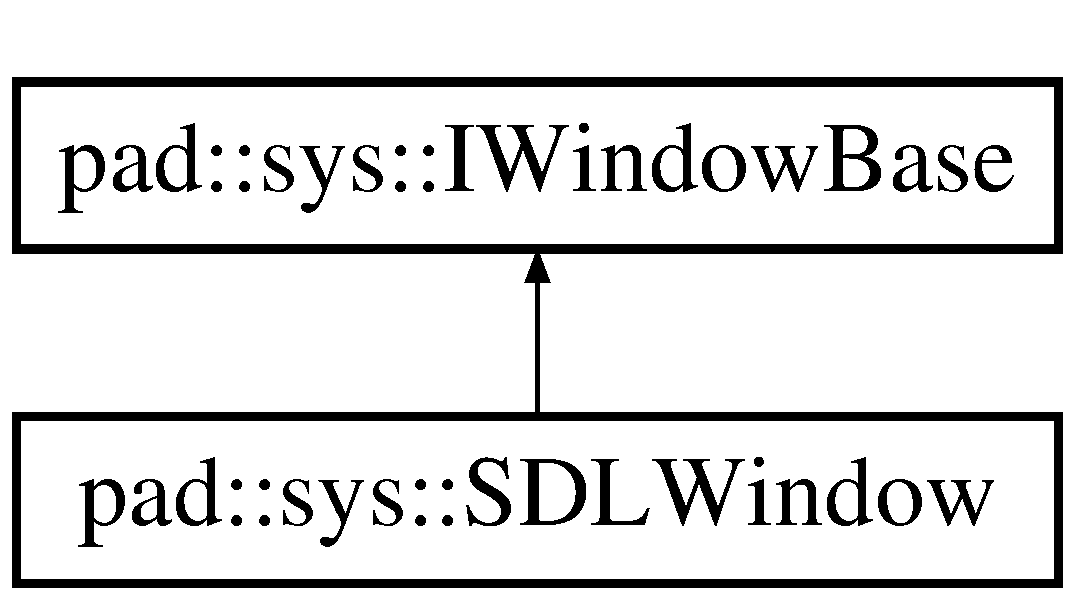
\includegraphics[height=2.000000cm]{classpad_1_1sys_1_1_s_d_l_window}
\end{center}
\end{figure}
\subsection*{Public Member Functions}
\begin{DoxyCompactItemize}
\item 
\mbox{\hyperlink{classpad_1_1sys_1_1_s_d_l_window_a545ce6b68cf03a84e5602e073f2edf99}{S\+D\+L\+Window}} ()
\item 
virtual \mbox{\hyperlink{classpad_1_1sys_1_1_s_d_l_window_a7baa8b1db939c5e1dab0cf19d9fe471a}{$\sim$\+S\+D\+L\+Window}} ()
\item 
\mbox{\hyperlink{classpad_1_1sys_1_1_s_d_l_window_a48fdb9ea4f9d04e0e85be929b485417b}{S\+D\+L\+Window}} (const \mbox{\hyperlink{classpad_1_1sys_1_1_s_d_l_window}{S\+D\+L\+Window}} \&)=delete
\item 
\mbox{\hyperlink{classpad_1_1sys_1_1_s_d_l_window_a2c16cacdc5ab08b8d84e00f287cab5ad}{S\+D\+L\+Window}} (\mbox{\hyperlink{classpad_1_1sys_1_1_s_d_l_window}{S\+D\+L\+Window}} \&\&)=delete
\item 
virtual void \mbox{\hyperlink{classpad_1_1sys_1_1_s_d_l_window_a7749e49f614ac33a95f1ef4ffed853e7}{Init}} (const \mbox{\hyperlink{structpad_1_1sys_1_1_window_settings}{Window\+Settings}} \&\+\_\+infos)
\item 
virtual void \mbox{\hyperlink{classpad_1_1sys_1_1_s_d_l_window_a66014e181e30c20a3488ff715d106665}{Poll\+Events}} ()
\item 
virtual void \mbox{\hyperlink{classpad_1_1sys_1_1_s_d_l_window_aba5a51090a6865da6d47826af28413ef}{Resize}} (const \mbox{\hyperlink{namespacepad_1_1math_a9773bcf81aa2ddd829bc327d822c6552}{math\+::\+Vec2}}$<$ \mbox{\hyperlink{namespacepad_a03b9241a5f6a191da2faac64714e1038}{uint16}} $>$ \&size)
\item 
virtual void \mbox{\hyperlink{classpad_1_1sys_1_1_s_d_l_window_a7f45cd8f1ffa83c4aaedf40b69012870}{Reload\+Settings}} (const \mbox{\hyperlink{structpad_1_1sys_1_1_window_settings}{Window\+Settings}} \&\+\_\+infos)
\item 
virtual void \mbox{\hyperlink{classpad_1_1sys_1_1_s_d_l_window_a991b47b499f3073e4d1962c2512e2ae8}{Swap\+Buffer}} ()
\item 
virtual bool \mbox{\hyperlink{classpad_1_1sys_1_1_s_d_l_window_ae76d9066f3c36e8b949b6c211be0affd}{Is\+Open}} ()
\item 
virtual const \mbox{\hyperlink{namespacepad_1_1math_a808a631a6bccd994f9589d7fb86bad41}{math\+::\+Vec2i}} \mbox{\hyperlink{classpad_1_1sys_1_1_s_d_l_window_a43391052519ec0bc8c194642d6d68d12}{Get\+Position}} () const
\item 
virtual const \mbox{\hyperlink{namespacepad_1_1math_a808a631a6bccd994f9589d7fb86bad41}{math\+::\+Vec2i}} \mbox{\hyperlink{classpad_1_1sys_1_1_s_d_l_window_a4b39d8767776e1fe6f613ad3fe7d7b29}{Get\+Size}} () const
\item 
\mbox{\hyperlink{classpad_1_1sys_1_1_s_d_l_window}{S\+D\+L\+Window}} \& \mbox{\hyperlink{classpad_1_1sys_1_1_s_d_l_window_a16ec17984ff879debe4ddce2784ec858}{operator=}} (const \mbox{\hyperlink{classpad_1_1sys_1_1_s_d_l_window}{S\+D\+L\+Window}} \&)=delete
\item 
\mbox{\hyperlink{classpad_1_1sys_1_1_s_d_l_window}{S\+D\+L\+Window}} \& \mbox{\hyperlink{classpad_1_1sys_1_1_s_d_l_window_addbf3af44214f1bc0ece277fedac35cd}{operator=}} (\mbox{\hyperlink{classpad_1_1sys_1_1_s_d_l_window}{S\+D\+L\+Window}} \&\&)=delete
\end{DoxyCompactItemize}
\subsection*{Private Attributes}
\begin{DoxyCompactItemize}
\item 
S\+D\+L\+\_\+\+Window $\ast$ \mbox{\hyperlink{classpad_1_1sys_1_1_s_d_l_window_a9ca166466e5306a205a3448d4199ec4f}{mp\+\_\+window}}
\item 
S\+D\+L\+\_\+\+G\+L\+Context \mbox{\hyperlink{classpad_1_1sys_1_1_s_d_l_window_a96971350b1dc47be7cd0ef7776ae095f}{m\+\_\+context}}
\item 
S\+D\+L\+\_\+\+Event \mbox{\hyperlink{classpad_1_1sys_1_1_s_d_l_window_a98bb97af76c295e146a2237147150545}{m\+\_\+event}}
\end{DoxyCompactItemize}
\subsection*{Additional Inherited Members}


\subsection{Constructor \& Destructor Documentation}
\mbox{\Hypertarget{classpad_1_1sys_1_1_s_d_l_window_a545ce6b68cf03a84e5602e073f2edf99}\label{classpad_1_1sys_1_1_s_d_l_window_a545ce6b68cf03a84e5602e073f2edf99}} 
\index{pad\+::sys\+::\+S\+D\+L\+Window@{pad\+::sys\+::\+S\+D\+L\+Window}!S\+D\+L\+Window@{S\+D\+L\+Window}}
\index{S\+D\+L\+Window@{S\+D\+L\+Window}!pad\+::sys\+::\+S\+D\+L\+Window@{pad\+::sys\+::\+S\+D\+L\+Window}}
\subsubsection{\texorpdfstring{S\+D\+L\+Window()}{SDLWindow()}\hspace{0.1cm}{\footnotesize\ttfamily [1/3]}}
{\footnotesize\ttfamily pad\+::sys\+::\+S\+D\+L\+Window\+::\+S\+D\+L\+Window (\begin{DoxyParamCaption}{ }\end{DoxyParamCaption})}

\mbox{\Hypertarget{classpad_1_1sys_1_1_s_d_l_window_a7baa8b1db939c5e1dab0cf19d9fe471a}\label{classpad_1_1sys_1_1_s_d_l_window_a7baa8b1db939c5e1dab0cf19d9fe471a}} 
\index{pad\+::sys\+::\+S\+D\+L\+Window@{pad\+::sys\+::\+S\+D\+L\+Window}!````~S\+D\+L\+Window@{$\sim$\+S\+D\+L\+Window}}
\index{````~S\+D\+L\+Window@{$\sim$\+S\+D\+L\+Window}!pad\+::sys\+::\+S\+D\+L\+Window@{pad\+::sys\+::\+S\+D\+L\+Window}}
\subsubsection{\texorpdfstring{$\sim$\+S\+D\+L\+Window()}{~SDLWindow()}}
{\footnotesize\ttfamily pad\+::sys\+::\+S\+D\+L\+Window\+::$\sim$\+S\+D\+L\+Window (\begin{DoxyParamCaption}{ }\end{DoxyParamCaption})\hspace{0.3cm}{\ttfamily [virtual]}}

\mbox{\Hypertarget{classpad_1_1sys_1_1_s_d_l_window_a48fdb9ea4f9d04e0e85be929b485417b}\label{classpad_1_1sys_1_1_s_d_l_window_a48fdb9ea4f9d04e0e85be929b485417b}} 
\index{pad\+::sys\+::\+S\+D\+L\+Window@{pad\+::sys\+::\+S\+D\+L\+Window}!S\+D\+L\+Window@{S\+D\+L\+Window}}
\index{S\+D\+L\+Window@{S\+D\+L\+Window}!pad\+::sys\+::\+S\+D\+L\+Window@{pad\+::sys\+::\+S\+D\+L\+Window}}
\subsubsection{\texorpdfstring{S\+D\+L\+Window()}{SDLWindow()}\hspace{0.1cm}{\footnotesize\ttfamily [2/3]}}
{\footnotesize\ttfamily pad\+::sys\+::\+S\+D\+L\+Window\+::\+S\+D\+L\+Window (\begin{DoxyParamCaption}\item[{const \mbox{\hyperlink{classpad_1_1sys_1_1_s_d_l_window}{S\+D\+L\+Window}} \&}]{ }\end{DoxyParamCaption})\hspace{0.3cm}{\ttfamily [delete]}}

\mbox{\Hypertarget{classpad_1_1sys_1_1_s_d_l_window_a2c16cacdc5ab08b8d84e00f287cab5ad}\label{classpad_1_1sys_1_1_s_d_l_window_a2c16cacdc5ab08b8d84e00f287cab5ad}} 
\index{pad\+::sys\+::\+S\+D\+L\+Window@{pad\+::sys\+::\+S\+D\+L\+Window}!S\+D\+L\+Window@{S\+D\+L\+Window}}
\index{S\+D\+L\+Window@{S\+D\+L\+Window}!pad\+::sys\+::\+S\+D\+L\+Window@{pad\+::sys\+::\+S\+D\+L\+Window}}
\subsubsection{\texorpdfstring{S\+D\+L\+Window()}{SDLWindow()}\hspace{0.1cm}{\footnotesize\ttfamily [3/3]}}
{\footnotesize\ttfamily pad\+::sys\+::\+S\+D\+L\+Window\+::\+S\+D\+L\+Window (\begin{DoxyParamCaption}\item[{\mbox{\hyperlink{classpad_1_1sys_1_1_s_d_l_window}{S\+D\+L\+Window}} \&\&}]{ }\end{DoxyParamCaption})\hspace{0.3cm}{\ttfamily [delete]}}



\subsection{Member Function Documentation}
\mbox{\Hypertarget{classpad_1_1sys_1_1_s_d_l_window_a43391052519ec0bc8c194642d6d68d12}\label{classpad_1_1sys_1_1_s_d_l_window_a43391052519ec0bc8c194642d6d68d12}} 
\index{pad\+::sys\+::\+S\+D\+L\+Window@{pad\+::sys\+::\+S\+D\+L\+Window}!Get\+Position@{Get\+Position}}
\index{Get\+Position@{Get\+Position}!pad\+::sys\+::\+S\+D\+L\+Window@{pad\+::sys\+::\+S\+D\+L\+Window}}
\subsubsection{\texorpdfstring{Get\+Position()}{GetPosition()}}
{\footnotesize\ttfamily virtual const \mbox{\hyperlink{namespacepad_1_1math_a808a631a6bccd994f9589d7fb86bad41}{math\+::\+Vec2i}} pad\+::sys\+::\+S\+D\+L\+Window\+::\+Get\+Position (\begin{DoxyParamCaption}{ }\end{DoxyParamCaption}) const\hspace{0.3cm}{\ttfamily [inline]}, {\ttfamily [virtual]}}



Implements \mbox{\hyperlink{classpad_1_1sys_1_1_i_window_base_ac3cb42c492b8c2ba59f36da4702b7bec}{pad\+::sys\+::\+I\+Window\+Base}}.

\mbox{\Hypertarget{classpad_1_1sys_1_1_s_d_l_window_a4b39d8767776e1fe6f613ad3fe7d7b29}\label{classpad_1_1sys_1_1_s_d_l_window_a4b39d8767776e1fe6f613ad3fe7d7b29}} 
\index{pad\+::sys\+::\+S\+D\+L\+Window@{pad\+::sys\+::\+S\+D\+L\+Window}!Get\+Size@{Get\+Size}}
\index{Get\+Size@{Get\+Size}!pad\+::sys\+::\+S\+D\+L\+Window@{pad\+::sys\+::\+S\+D\+L\+Window}}
\subsubsection{\texorpdfstring{Get\+Size()}{GetSize()}}
{\footnotesize\ttfamily virtual const \mbox{\hyperlink{namespacepad_1_1math_a808a631a6bccd994f9589d7fb86bad41}{math\+::\+Vec2i}} pad\+::sys\+::\+S\+D\+L\+Window\+::\+Get\+Size (\begin{DoxyParamCaption}{ }\end{DoxyParamCaption}) const\hspace{0.3cm}{\ttfamily [inline]}, {\ttfamily [virtual]}}



Implements \mbox{\hyperlink{classpad_1_1sys_1_1_i_window_base_acf3540e89da05cc490cf981f196ad771}{pad\+::sys\+::\+I\+Window\+Base}}.

\mbox{\Hypertarget{classpad_1_1sys_1_1_s_d_l_window_a7749e49f614ac33a95f1ef4ffed853e7}\label{classpad_1_1sys_1_1_s_d_l_window_a7749e49f614ac33a95f1ef4ffed853e7}} 
\index{pad\+::sys\+::\+S\+D\+L\+Window@{pad\+::sys\+::\+S\+D\+L\+Window}!Init@{Init}}
\index{Init@{Init}!pad\+::sys\+::\+S\+D\+L\+Window@{pad\+::sys\+::\+S\+D\+L\+Window}}
\subsubsection{\texorpdfstring{Init()}{Init()}}
{\footnotesize\ttfamily void pad\+::sys\+::\+S\+D\+L\+Window\+::\+Init (\begin{DoxyParamCaption}\item[{const \mbox{\hyperlink{structpad_1_1sys_1_1_window_settings}{Window\+Settings}} \&}]{\+\_\+infos }\end{DoxyParamCaption})\hspace{0.3cm}{\ttfamily [virtual]}}



Implements \mbox{\hyperlink{classpad_1_1sys_1_1_i_window_base_aee66a6eacff6126f4106a8e725bcbf1f}{pad\+::sys\+::\+I\+Window\+Base}}.

\mbox{\Hypertarget{classpad_1_1sys_1_1_s_d_l_window_ae76d9066f3c36e8b949b6c211be0affd}\label{classpad_1_1sys_1_1_s_d_l_window_ae76d9066f3c36e8b949b6c211be0affd}} 
\index{pad\+::sys\+::\+S\+D\+L\+Window@{pad\+::sys\+::\+S\+D\+L\+Window}!Is\+Open@{Is\+Open}}
\index{Is\+Open@{Is\+Open}!pad\+::sys\+::\+S\+D\+L\+Window@{pad\+::sys\+::\+S\+D\+L\+Window}}
\subsubsection{\texorpdfstring{Is\+Open()}{IsOpen()}}
{\footnotesize\ttfamily virtual bool pad\+::sys\+::\+S\+D\+L\+Window\+::\+Is\+Open (\begin{DoxyParamCaption}{ }\end{DoxyParamCaption})\hspace{0.3cm}{\ttfamily [inline]}, {\ttfamily [virtual]}}



Implements \mbox{\hyperlink{classpad_1_1sys_1_1_i_window_base_a07aae1254b0d8139e912584029d785ea}{pad\+::sys\+::\+I\+Window\+Base}}.

\mbox{\Hypertarget{classpad_1_1sys_1_1_s_d_l_window_a16ec17984ff879debe4ddce2784ec858}\label{classpad_1_1sys_1_1_s_d_l_window_a16ec17984ff879debe4ddce2784ec858}} 
\index{pad\+::sys\+::\+S\+D\+L\+Window@{pad\+::sys\+::\+S\+D\+L\+Window}!operator=@{operator=}}
\index{operator=@{operator=}!pad\+::sys\+::\+S\+D\+L\+Window@{pad\+::sys\+::\+S\+D\+L\+Window}}
\subsubsection{\texorpdfstring{operator=()}{operator=()}\hspace{0.1cm}{\footnotesize\ttfamily [1/2]}}
{\footnotesize\ttfamily \mbox{\hyperlink{classpad_1_1sys_1_1_s_d_l_window}{S\+D\+L\+Window}}\& pad\+::sys\+::\+S\+D\+L\+Window\+::operator= (\begin{DoxyParamCaption}\item[{const \mbox{\hyperlink{classpad_1_1sys_1_1_s_d_l_window}{S\+D\+L\+Window}} \&}]{ }\end{DoxyParamCaption})\hspace{0.3cm}{\ttfamily [delete]}}

\mbox{\Hypertarget{classpad_1_1sys_1_1_s_d_l_window_addbf3af44214f1bc0ece277fedac35cd}\label{classpad_1_1sys_1_1_s_d_l_window_addbf3af44214f1bc0ece277fedac35cd}} 
\index{pad\+::sys\+::\+S\+D\+L\+Window@{pad\+::sys\+::\+S\+D\+L\+Window}!operator=@{operator=}}
\index{operator=@{operator=}!pad\+::sys\+::\+S\+D\+L\+Window@{pad\+::sys\+::\+S\+D\+L\+Window}}
\subsubsection{\texorpdfstring{operator=()}{operator=()}\hspace{0.1cm}{\footnotesize\ttfamily [2/2]}}
{\footnotesize\ttfamily \mbox{\hyperlink{classpad_1_1sys_1_1_s_d_l_window}{S\+D\+L\+Window}}\& pad\+::sys\+::\+S\+D\+L\+Window\+::operator= (\begin{DoxyParamCaption}\item[{\mbox{\hyperlink{classpad_1_1sys_1_1_s_d_l_window}{S\+D\+L\+Window}} \&\&}]{ }\end{DoxyParamCaption})\hspace{0.3cm}{\ttfamily [delete]}}

\mbox{\Hypertarget{classpad_1_1sys_1_1_s_d_l_window_a66014e181e30c20a3488ff715d106665}\label{classpad_1_1sys_1_1_s_d_l_window_a66014e181e30c20a3488ff715d106665}} 
\index{pad\+::sys\+::\+S\+D\+L\+Window@{pad\+::sys\+::\+S\+D\+L\+Window}!Poll\+Events@{Poll\+Events}}
\index{Poll\+Events@{Poll\+Events}!pad\+::sys\+::\+S\+D\+L\+Window@{pad\+::sys\+::\+S\+D\+L\+Window}}
\subsubsection{\texorpdfstring{Poll\+Events()}{PollEvents()}}
{\footnotesize\ttfamily void pad\+::sys\+::\+S\+D\+L\+Window\+::\+Poll\+Events (\begin{DoxyParamCaption}{ }\end{DoxyParamCaption})\hspace{0.3cm}{\ttfamily [virtual]}}



Implements \mbox{\hyperlink{classpad_1_1sys_1_1_i_window_base_aee21db35ea6bdd4299783b4e96a9b326}{pad\+::sys\+::\+I\+Window\+Base}}.

\mbox{\Hypertarget{classpad_1_1sys_1_1_s_d_l_window_a7f45cd8f1ffa83c4aaedf40b69012870}\label{classpad_1_1sys_1_1_s_d_l_window_a7f45cd8f1ffa83c4aaedf40b69012870}} 
\index{pad\+::sys\+::\+S\+D\+L\+Window@{pad\+::sys\+::\+S\+D\+L\+Window}!Reload\+Settings@{Reload\+Settings}}
\index{Reload\+Settings@{Reload\+Settings}!pad\+::sys\+::\+S\+D\+L\+Window@{pad\+::sys\+::\+S\+D\+L\+Window}}
\subsubsection{\texorpdfstring{Reload\+Settings()}{ReloadSettings()}}
{\footnotesize\ttfamily void pad\+::sys\+::\+S\+D\+L\+Window\+::\+Reload\+Settings (\begin{DoxyParamCaption}\item[{const \mbox{\hyperlink{structpad_1_1sys_1_1_window_settings}{Window\+Settings}} \&}]{\+\_\+infos }\end{DoxyParamCaption})\hspace{0.3cm}{\ttfamily [virtual]}}



Implements \mbox{\hyperlink{classpad_1_1sys_1_1_i_window_base_aff693c784fbf16ae5bbfce797f570879}{pad\+::sys\+::\+I\+Window\+Base}}.

\mbox{\Hypertarget{classpad_1_1sys_1_1_s_d_l_window_aba5a51090a6865da6d47826af28413ef}\label{classpad_1_1sys_1_1_s_d_l_window_aba5a51090a6865da6d47826af28413ef}} 
\index{pad\+::sys\+::\+S\+D\+L\+Window@{pad\+::sys\+::\+S\+D\+L\+Window}!Resize@{Resize}}
\index{Resize@{Resize}!pad\+::sys\+::\+S\+D\+L\+Window@{pad\+::sys\+::\+S\+D\+L\+Window}}
\subsubsection{\texorpdfstring{Resize()}{Resize()}}
{\footnotesize\ttfamily void pad\+::sys\+::\+S\+D\+L\+Window\+::\+Resize (\begin{DoxyParamCaption}\item[{const \mbox{\hyperlink{namespacepad_1_1math_a9773bcf81aa2ddd829bc327d822c6552}{math\+::\+Vec2}}$<$ \mbox{\hyperlink{namespacepad_a03b9241a5f6a191da2faac64714e1038}{uint16}} $>$ \&}]{size }\end{DoxyParamCaption})\hspace{0.3cm}{\ttfamily [virtual]}}



Implements \mbox{\hyperlink{classpad_1_1sys_1_1_i_window_base_a19fff5f21c5a75082d8ca4e2491b269e}{pad\+::sys\+::\+I\+Window\+Base}}.

\mbox{\Hypertarget{classpad_1_1sys_1_1_s_d_l_window_a991b47b499f3073e4d1962c2512e2ae8}\label{classpad_1_1sys_1_1_s_d_l_window_a991b47b499f3073e4d1962c2512e2ae8}} 
\index{pad\+::sys\+::\+S\+D\+L\+Window@{pad\+::sys\+::\+S\+D\+L\+Window}!Swap\+Buffer@{Swap\+Buffer}}
\index{Swap\+Buffer@{Swap\+Buffer}!pad\+::sys\+::\+S\+D\+L\+Window@{pad\+::sys\+::\+S\+D\+L\+Window}}
\subsubsection{\texorpdfstring{Swap\+Buffer()}{SwapBuffer()}}
{\footnotesize\ttfamily void pad\+::sys\+::\+S\+D\+L\+Window\+::\+Swap\+Buffer (\begin{DoxyParamCaption}{ }\end{DoxyParamCaption})\hspace{0.3cm}{\ttfamily [virtual]}}



Implements \mbox{\hyperlink{classpad_1_1sys_1_1_i_window_base_ac6fe9dea946b20c52ad8d9372e57e6c1}{pad\+::sys\+::\+I\+Window\+Base}}.



\subsection{Member Data Documentation}
\mbox{\Hypertarget{classpad_1_1sys_1_1_s_d_l_window_a96971350b1dc47be7cd0ef7776ae095f}\label{classpad_1_1sys_1_1_s_d_l_window_a96971350b1dc47be7cd0ef7776ae095f}} 
\index{pad\+::sys\+::\+S\+D\+L\+Window@{pad\+::sys\+::\+S\+D\+L\+Window}!m\+\_\+context@{m\+\_\+context}}
\index{m\+\_\+context@{m\+\_\+context}!pad\+::sys\+::\+S\+D\+L\+Window@{pad\+::sys\+::\+S\+D\+L\+Window}}
\subsubsection{\texorpdfstring{m\+\_\+context}{m\_context}}
{\footnotesize\ttfamily S\+D\+L\+\_\+\+G\+L\+Context pad\+::sys\+::\+S\+D\+L\+Window\+::m\+\_\+context\hspace{0.3cm}{\ttfamily [private]}}

\mbox{\Hypertarget{classpad_1_1sys_1_1_s_d_l_window_a98bb97af76c295e146a2237147150545}\label{classpad_1_1sys_1_1_s_d_l_window_a98bb97af76c295e146a2237147150545}} 
\index{pad\+::sys\+::\+S\+D\+L\+Window@{pad\+::sys\+::\+S\+D\+L\+Window}!m\+\_\+event@{m\+\_\+event}}
\index{m\+\_\+event@{m\+\_\+event}!pad\+::sys\+::\+S\+D\+L\+Window@{pad\+::sys\+::\+S\+D\+L\+Window}}
\subsubsection{\texorpdfstring{m\+\_\+event}{m\_event}}
{\footnotesize\ttfamily S\+D\+L\+\_\+\+Event pad\+::sys\+::\+S\+D\+L\+Window\+::m\+\_\+event\hspace{0.3cm}{\ttfamily [private]}}

\mbox{\Hypertarget{classpad_1_1sys_1_1_s_d_l_window_a9ca166466e5306a205a3448d4199ec4f}\label{classpad_1_1sys_1_1_s_d_l_window_a9ca166466e5306a205a3448d4199ec4f}} 
\index{pad\+::sys\+::\+S\+D\+L\+Window@{pad\+::sys\+::\+S\+D\+L\+Window}!mp\+\_\+window@{mp\+\_\+window}}
\index{mp\+\_\+window@{mp\+\_\+window}!pad\+::sys\+::\+S\+D\+L\+Window@{pad\+::sys\+::\+S\+D\+L\+Window}}
\subsubsection{\texorpdfstring{mp\+\_\+window}{mp\_window}}
{\footnotesize\ttfamily S\+D\+L\+\_\+\+Window$\ast$ pad\+::sys\+::\+S\+D\+L\+Window\+::mp\+\_\+window\hspace{0.3cm}{\ttfamily [private]}}



The documentation for this class was generated from the following files\+:\begin{DoxyCompactItemize}
\item 
P\+A\+D Engine/\+Sources/\+System/\mbox{\hyperlink{_s_d_l_window_8h}{S\+D\+L\+Window.\+h}}\item 
P\+A\+D Engine/\+Sources/\+System/\mbox{\hyperlink{_s_d_l_window_8cpp}{S\+D\+L\+Window.\+cpp}}\end{DoxyCompactItemize}

\hypertarget{classpad_1_1gfx_1_1_shader}{}\section{pad\+:\+:gfx\+:\+:Shader Class Reference}
\label{classpad_1_1gfx_1_1_shader}\index{pad\+::gfx\+::\+Shader@{pad\+::gfx\+::\+Shader}}


{\ttfamily \#include $<$Shader.\+h$>$}

\subsection*{Public Member Functions}
\begin{DoxyCompactItemize}
\item 
\mbox{\hyperlink{classpad_1_1gfx_1_1_shader_a4586e58e09b934d75f84008cf54cd2d7}{Shader}} ()
\item 
\mbox{\hyperlink{classpad_1_1gfx_1_1_shader_ac920a092249199c7d3d4c44d60aeb3d0}{$\sim$\+Shader}} ()=default
\item 
\mbox{\hyperlink{classpad_1_1gfx_1_1_shader_a1d86c13c0a18fb940f8e30870422f51c}{Shader}} (const \mbox{\hyperlink{classpad_1_1gfx_1_1_shader}{Shader}} \&)=delete
\item 
\mbox{\hyperlink{classpad_1_1gfx_1_1_shader_aeb647f99ec9239504b648be1434be6a3}{Shader}} (\mbox{\hyperlink{classpad_1_1gfx_1_1_shader}{Shader}} \&\&)=delete
\item 
void \mbox{\hyperlink{classpad_1_1gfx_1_1_shader_a92b1501375147c0763a50c3b60c6819b}{Use}} ()
\item 
bool \mbox{\hyperlink{classpad_1_1gfx_1_1_shader_af1232aebd7859cd712cd5dbc08c05f32}{Load\+From\+File}} (const char $\ast$\+\_\+v\+Path, const char $\ast$\+\_\+f\+Path)
\item 
void \mbox{\hyperlink{classpad_1_1gfx_1_1_shader_a2166cedcae52902649e267c1927d0272}{operator=}} (const \mbox{\hyperlink{classpad_1_1gfx_1_1_shader}{Shader}} \&)=delete
\item 
void \mbox{\hyperlink{classpad_1_1gfx_1_1_shader_a7b32b62ff74e9081d01f806b22c2f014}{operator=}} (\mbox{\hyperlink{classpad_1_1gfx_1_1_shader}{Shader}} \&\&)=delete
\end{DoxyCompactItemize}
\subsection*{Private Member Functions}
\begin{DoxyCompactItemize}
\item 
bool \mbox{\hyperlink{classpad_1_1gfx_1_1_shader_a17edbaae92b607880efa4e79a5a6adb9}{Compile\+Shader}} (const char $\ast$\+\_\+shader\+Code, \mbox{\hyperlink{namespacepad_a7faacd72761782d8adef66f2feba3c21}{int32}} \&\+\_\+shader\+ID, const \mbox{\hyperlink{namespacepad_1_1gfx_a04785a7d8a9087a9f0f2459a99a068a6}{E\+\_\+\+S\+H\+A\+D\+E\+R\+\_\+\+T\+Y\+PE}} \&\+\_\+type)
\item 
bool \mbox{\hyperlink{classpad_1_1gfx_1_1_shader_a4adbd190355e4920d4739130d651778a}{Load\+Shader}} (const char $\ast$\+\_\+path, const \mbox{\hyperlink{namespacepad_1_1gfx_a04785a7d8a9087a9f0f2459a99a068a6}{E\+\_\+\+S\+H\+A\+D\+E\+R\+\_\+\+T\+Y\+PE}} \&\+\_\+type, \mbox{\hyperlink{namespacepad_a7faacd72761782d8adef66f2feba3c21}{int32}} \&\+\_\+shader\+ID)
\item 
bool \mbox{\hyperlink{classpad_1_1gfx_1_1_shader_a79cc2be52055b9801745cd17e58b1b13}{Create\+Program}} (const \mbox{\hyperlink{namespacepad_a7faacd72761782d8adef66f2feba3c21}{int32}} \+\_\+vert\+ID, const \mbox{\hyperlink{namespacepad_a7faacd72761782d8adef66f2feba3c21}{int32}} \+\_\+frag\+ID)
\end{DoxyCompactItemize}
\subsection*{Private Attributes}
\begin{DoxyCompactItemize}
\item 
\mbox{\hyperlink{namespacepad_a7faacd72761782d8adef66f2feba3c21}{int32}} \mbox{\hyperlink{classpad_1_1gfx_1_1_shader_aad9b828da5a2b4c510a186f23f2cb633}{m\+\_\+prog\+ID}}
\end{DoxyCompactItemize}
\subsection*{Static Private Attributes}
\begin{DoxyCompactItemize}
\item 
static \mbox{\hyperlink{namespacepad_a7faacd72761782d8adef66f2feba3c21}{int32}} \mbox{\hyperlink{classpad_1_1gfx_1_1_shader_ad9eaa6681fa2cc603230d1ed006c6fe3}{m\+\_\+current\+Prog\+ID}} = \mbox{\hyperlink{_shader_8cpp_a9fe0beb08874420b17d7de8e9479f59c}{I\+N\+V\+A\+L\+I\+D\+\_\+\+P\+R\+O\+G\+\_\+\+V\+A\+L\+UE}}
\end{DoxyCompactItemize}


\subsection{Constructor \& Destructor Documentation}
\mbox{\Hypertarget{classpad_1_1gfx_1_1_shader_a4586e58e09b934d75f84008cf54cd2d7}\label{classpad_1_1gfx_1_1_shader_a4586e58e09b934d75f84008cf54cd2d7}} 
\index{pad\+::gfx\+::\+Shader@{pad\+::gfx\+::\+Shader}!Shader@{Shader}}
\index{Shader@{Shader}!pad\+::gfx\+::\+Shader@{pad\+::gfx\+::\+Shader}}
\subsubsection{\texorpdfstring{Shader()}{Shader()}\hspace{0.1cm}{\footnotesize\ttfamily [1/3]}}
{\footnotesize\ttfamily pad\+::gfx\+::\+Shader\+::\+Shader (\begin{DoxyParamCaption}{ }\end{DoxyParamCaption})}

\mbox{\Hypertarget{classpad_1_1gfx_1_1_shader_ac920a092249199c7d3d4c44d60aeb3d0}\label{classpad_1_1gfx_1_1_shader_ac920a092249199c7d3d4c44d60aeb3d0}} 
\index{pad\+::gfx\+::\+Shader@{pad\+::gfx\+::\+Shader}!````~Shader@{$\sim$\+Shader}}
\index{````~Shader@{$\sim$\+Shader}!pad\+::gfx\+::\+Shader@{pad\+::gfx\+::\+Shader}}
\subsubsection{\texorpdfstring{$\sim$\+Shader()}{~Shader()}}
{\footnotesize\ttfamily pad\+::gfx\+::\+Shader\+::$\sim$\+Shader (\begin{DoxyParamCaption}{ }\end{DoxyParamCaption})\hspace{0.3cm}{\ttfamily [default]}}

\mbox{\Hypertarget{classpad_1_1gfx_1_1_shader_a1d86c13c0a18fb940f8e30870422f51c}\label{classpad_1_1gfx_1_1_shader_a1d86c13c0a18fb940f8e30870422f51c}} 
\index{pad\+::gfx\+::\+Shader@{pad\+::gfx\+::\+Shader}!Shader@{Shader}}
\index{Shader@{Shader}!pad\+::gfx\+::\+Shader@{pad\+::gfx\+::\+Shader}}
\subsubsection{\texorpdfstring{Shader()}{Shader()}\hspace{0.1cm}{\footnotesize\ttfamily [2/3]}}
{\footnotesize\ttfamily pad\+::gfx\+::\+Shader\+::\+Shader (\begin{DoxyParamCaption}\item[{const \mbox{\hyperlink{classpad_1_1gfx_1_1_shader}{Shader}} \&}]{ }\end{DoxyParamCaption})\hspace{0.3cm}{\ttfamily [delete]}}

\mbox{\Hypertarget{classpad_1_1gfx_1_1_shader_aeb647f99ec9239504b648be1434be6a3}\label{classpad_1_1gfx_1_1_shader_aeb647f99ec9239504b648be1434be6a3}} 
\index{pad\+::gfx\+::\+Shader@{pad\+::gfx\+::\+Shader}!Shader@{Shader}}
\index{Shader@{Shader}!pad\+::gfx\+::\+Shader@{pad\+::gfx\+::\+Shader}}
\subsubsection{\texorpdfstring{Shader()}{Shader()}\hspace{0.1cm}{\footnotesize\ttfamily [3/3]}}
{\footnotesize\ttfamily pad\+::gfx\+::\+Shader\+::\+Shader (\begin{DoxyParamCaption}\item[{\mbox{\hyperlink{classpad_1_1gfx_1_1_shader}{Shader}} \&\&}]{ }\end{DoxyParamCaption})\hspace{0.3cm}{\ttfamily [delete]}}



\subsection{Member Function Documentation}
\mbox{\Hypertarget{classpad_1_1gfx_1_1_shader_a17edbaae92b607880efa4e79a5a6adb9}\label{classpad_1_1gfx_1_1_shader_a17edbaae92b607880efa4e79a5a6adb9}} 
\index{pad\+::gfx\+::\+Shader@{pad\+::gfx\+::\+Shader}!Compile\+Shader@{Compile\+Shader}}
\index{Compile\+Shader@{Compile\+Shader}!pad\+::gfx\+::\+Shader@{pad\+::gfx\+::\+Shader}}
\subsubsection{\texorpdfstring{Compile\+Shader()}{CompileShader()}}
{\footnotesize\ttfamily bool pad\+::gfx\+::\+Shader\+::\+Compile\+Shader (\begin{DoxyParamCaption}\item[{const char $\ast$}]{\+\_\+shader\+Code,  }\item[{\mbox{\hyperlink{namespacepad_a7faacd72761782d8adef66f2feba3c21}{int32}} \&}]{\+\_\+shader\+ID,  }\item[{const \mbox{\hyperlink{namespacepad_1_1gfx_a04785a7d8a9087a9f0f2459a99a068a6}{E\+\_\+\+S\+H\+A\+D\+E\+R\+\_\+\+T\+Y\+PE}} \&}]{\+\_\+type }\end{DoxyParamCaption})\hspace{0.3cm}{\ttfamily [private]}}

\mbox{\Hypertarget{classpad_1_1gfx_1_1_shader_a79cc2be52055b9801745cd17e58b1b13}\label{classpad_1_1gfx_1_1_shader_a79cc2be52055b9801745cd17e58b1b13}} 
\index{pad\+::gfx\+::\+Shader@{pad\+::gfx\+::\+Shader}!Create\+Program@{Create\+Program}}
\index{Create\+Program@{Create\+Program}!pad\+::gfx\+::\+Shader@{pad\+::gfx\+::\+Shader}}
\subsubsection{\texorpdfstring{Create\+Program()}{CreateProgram()}}
{\footnotesize\ttfamily bool pad\+::gfx\+::\+Shader\+::\+Create\+Program (\begin{DoxyParamCaption}\item[{const \mbox{\hyperlink{namespacepad_a7faacd72761782d8adef66f2feba3c21}{int32}}}]{\+\_\+vert\+ID,  }\item[{const \mbox{\hyperlink{namespacepad_a7faacd72761782d8adef66f2feba3c21}{int32}}}]{\+\_\+frag\+ID }\end{DoxyParamCaption})\hspace{0.3cm}{\ttfamily [private]}}

\mbox{\Hypertarget{classpad_1_1gfx_1_1_shader_af1232aebd7859cd712cd5dbc08c05f32}\label{classpad_1_1gfx_1_1_shader_af1232aebd7859cd712cd5dbc08c05f32}} 
\index{pad\+::gfx\+::\+Shader@{pad\+::gfx\+::\+Shader}!Load\+From\+File@{Load\+From\+File}}
\index{Load\+From\+File@{Load\+From\+File}!pad\+::gfx\+::\+Shader@{pad\+::gfx\+::\+Shader}}
\subsubsection{\texorpdfstring{Load\+From\+File()}{LoadFromFile()}}
{\footnotesize\ttfamily bool pad\+::gfx\+::\+Shader\+::\+Load\+From\+File (\begin{DoxyParamCaption}\item[{const char $\ast$}]{\+\_\+v\+Path,  }\item[{const char $\ast$}]{\+\_\+f\+Path }\end{DoxyParamCaption})}

\mbox{\Hypertarget{classpad_1_1gfx_1_1_shader_a4adbd190355e4920d4739130d651778a}\label{classpad_1_1gfx_1_1_shader_a4adbd190355e4920d4739130d651778a}} 
\index{pad\+::gfx\+::\+Shader@{pad\+::gfx\+::\+Shader}!Load\+Shader@{Load\+Shader}}
\index{Load\+Shader@{Load\+Shader}!pad\+::gfx\+::\+Shader@{pad\+::gfx\+::\+Shader}}
\subsubsection{\texorpdfstring{Load\+Shader()}{LoadShader()}}
{\footnotesize\ttfamily bool pad\+::gfx\+::\+Shader\+::\+Load\+Shader (\begin{DoxyParamCaption}\item[{const char $\ast$}]{\+\_\+path,  }\item[{const \mbox{\hyperlink{namespacepad_1_1gfx_a04785a7d8a9087a9f0f2459a99a068a6}{E\+\_\+\+S\+H\+A\+D\+E\+R\+\_\+\+T\+Y\+PE}} \&}]{\+\_\+type,  }\item[{\mbox{\hyperlink{namespacepad_a7faacd72761782d8adef66f2feba3c21}{int32}} \&}]{\+\_\+shader\+ID }\end{DoxyParamCaption})\hspace{0.3cm}{\ttfamily [private]}}

\mbox{\Hypertarget{classpad_1_1gfx_1_1_shader_a2166cedcae52902649e267c1927d0272}\label{classpad_1_1gfx_1_1_shader_a2166cedcae52902649e267c1927d0272}} 
\index{pad\+::gfx\+::\+Shader@{pad\+::gfx\+::\+Shader}!operator=@{operator=}}
\index{operator=@{operator=}!pad\+::gfx\+::\+Shader@{pad\+::gfx\+::\+Shader}}
\subsubsection{\texorpdfstring{operator=()}{operator=()}\hspace{0.1cm}{\footnotesize\ttfamily [1/2]}}
{\footnotesize\ttfamily void pad\+::gfx\+::\+Shader\+::operator= (\begin{DoxyParamCaption}\item[{const \mbox{\hyperlink{classpad_1_1gfx_1_1_shader}{Shader}} \&}]{ }\end{DoxyParamCaption})\hspace{0.3cm}{\ttfamily [delete]}}

\mbox{\Hypertarget{classpad_1_1gfx_1_1_shader_a7b32b62ff74e9081d01f806b22c2f014}\label{classpad_1_1gfx_1_1_shader_a7b32b62ff74e9081d01f806b22c2f014}} 
\index{pad\+::gfx\+::\+Shader@{pad\+::gfx\+::\+Shader}!operator=@{operator=}}
\index{operator=@{operator=}!pad\+::gfx\+::\+Shader@{pad\+::gfx\+::\+Shader}}
\subsubsection{\texorpdfstring{operator=()}{operator=()}\hspace{0.1cm}{\footnotesize\ttfamily [2/2]}}
{\footnotesize\ttfamily void pad\+::gfx\+::\+Shader\+::operator= (\begin{DoxyParamCaption}\item[{\mbox{\hyperlink{classpad_1_1gfx_1_1_shader}{Shader}} \&\&}]{ }\end{DoxyParamCaption})\hspace{0.3cm}{\ttfamily [delete]}}

\mbox{\Hypertarget{classpad_1_1gfx_1_1_shader_a92b1501375147c0763a50c3b60c6819b}\label{classpad_1_1gfx_1_1_shader_a92b1501375147c0763a50c3b60c6819b}} 
\index{pad\+::gfx\+::\+Shader@{pad\+::gfx\+::\+Shader}!Use@{Use}}
\index{Use@{Use}!pad\+::gfx\+::\+Shader@{pad\+::gfx\+::\+Shader}}
\subsubsection{\texorpdfstring{Use()}{Use()}}
{\footnotesize\ttfamily void pad\+::gfx\+::\+Shader\+::\+Use (\begin{DoxyParamCaption}{ }\end{DoxyParamCaption})}



\subsection{Member Data Documentation}
\mbox{\Hypertarget{classpad_1_1gfx_1_1_shader_ad9eaa6681fa2cc603230d1ed006c6fe3}\label{classpad_1_1gfx_1_1_shader_ad9eaa6681fa2cc603230d1ed006c6fe3}} 
\index{pad\+::gfx\+::\+Shader@{pad\+::gfx\+::\+Shader}!m\+\_\+current\+Prog\+ID@{m\+\_\+current\+Prog\+ID}}
\index{m\+\_\+current\+Prog\+ID@{m\+\_\+current\+Prog\+ID}!pad\+::gfx\+::\+Shader@{pad\+::gfx\+::\+Shader}}
\subsubsection{\texorpdfstring{m\+\_\+current\+Prog\+ID}{m\_currentProgID}}
{\footnotesize\ttfamily \mbox{\hyperlink{namespacepad_a7faacd72761782d8adef66f2feba3c21}{int32}} pad\+::gfx\+::\+Shader\+::m\+\_\+current\+Prog\+ID = \mbox{\hyperlink{_shader_8cpp_a9fe0beb08874420b17d7de8e9479f59c}{I\+N\+V\+A\+L\+I\+D\+\_\+\+P\+R\+O\+G\+\_\+\+V\+A\+L\+UE}}\hspace{0.3cm}{\ttfamily [static]}, {\ttfamily [private]}}

\mbox{\Hypertarget{classpad_1_1gfx_1_1_shader_aad9b828da5a2b4c510a186f23f2cb633}\label{classpad_1_1gfx_1_1_shader_aad9b828da5a2b4c510a186f23f2cb633}} 
\index{pad\+::gfx\+::\+Shader@{pad\+::gfx\+::\+Shader}!m\+\_\+prog\+ID@{m\+\_\+prog\+ID}}
\index{m\+\_\+prog\+ID@{m\+\_\+prog\+ID}!pad\+::gfx\+::\+Shader@{pad\+::gfx\+::\+Shader}}
\subsubsection{\texorpdfstring{m\+\_\+prog\+ID}{m\_progID}}
{\footnotesize\ttfamily \mbox{\hyperlink{namespacepad_a7faacd72761782d8adef66f2feba3c21}{int32}} pad\+::gfx\+::\+Shader\+::m\+\_\+prog\+ID\hspace{0.3cm}{\ttfamily [private]}}



The documentation for this class was generated from the following files\+:\begin{DoxyCompactItemize}
\item 
P\+A\+D Engine/\+Sources/\+Graphics/\mbox{\hyperlink{_shader_8h}{Shader.\+h}}\item 
P\+A\+D Engine/\+Sources/\+Graphics/\mbox{\hyperlink{_shader_8cpp}{Shader.\+cpp}}\end{DoxyCompactItemize}

\hypertarget{classpad_1_1core_1_1_timer}{}\section{pad\+:\+:core\+:\+:Timer Class Reference}
\label{classpad_1_1core_1_1_timer}\index{pad\+::core\+::\+Timer@{pad\+::core\+::\+Timer}}


{\ttfamily \#include $<$Timer.\+h$>$}

\subsection*{Public Member Functions}
\begin{DoxyCompactItemize}
\item 
\mbox{\hyperlink{classpad_1_1core_1_1_timer_a30a7706137aea9acde41ca7ee90326e3}{Timer}} (const bool \+\_\+affected\+By\+Pause=true)
\item 
\mbox{\hyperlink{classpad_1_1core_1_1_timer_aec538febc2d52e50ad5df1b200b60d5d}{$\sim$\+Timer}} ()
\item 
void \mbox{\hyperlink{classpad_1_1core_1_1_timer_ac3c92037256639490ad979987c58a3d3}{Start}} ()
\item 
void \mbox{\hyperlink{classpad_1_1core_1_1_timer_a150118ce8a2eaa2aa2e5e827511356f9}{Pause}} ()
\item 
void \mbox{\hyperlink{classpad_1_1core_1_1_timer_a06994d900c4a882acffc4ba47b99fc85}{Unpause}} ()
\item 
void \mbox{\hyperlink{classpad_1_1core_1_1_timer_a3a3cbda30033c7c9303f34ed103d70d8}{Stop}} ()
\item 
const double \mbox{\hyperlink{classpad_1_1core_1_1_timer_a81ee8c0bd00ea230edd6c177b578ae41}{Get\+Duration}} ()
\end{DoxyCompactItemize}
\subsection*{Private Attributes}
\begin{DoxyCompactItemize}
\item 
\mbox{\hyperlink{namespacepad_1_1core_a4359864da05f393ed6e69d9d018946ad}{Timepoint}} \mbox{\hyperlink{classpad_1_1core_1_1_timer_afe9926da78b47b4c3d33fab3632903a5}{start\+Time}}
\item 
double \mbox{\hyperlink{classpad_1_1core_1_1_timer_ad76d18dd62c6965847b39e4e1f5d0f9b}{duration}}
\item 
double \mbox{\hyperlink{classpad_1_1core_1_1_timer_a4c374309dd4560bb3203c79d5f41036c}{pause\+Duration}}
\item 
unsigned short \mbox{\hyperlink{classpad_1_1core_1_1_timer_a56bb681d982af55045a5f614ba5c9e22}{id}}
\item 
bool \mbox{\hyperlink{classpad_1_1core_1_1_timer_aaf3934066247c812ced8f0b234280925}{affected\+By\+Pause}}
\item 
\mbox{\hyperlink{namespacepad_1_1core_a4359864da05f393ed6e69d9d018946ad}{Timepoint}} \mbox{\hyperlink{classpad_1_1core_1_1_timer_a0cbad14aa307f3c039b0ac15c239078d}{pause\+Start\+Time}}
\end{DoxyCompactItemize}
\subsection*{Static Private Attributes}
\begin{DoxyCompactItemize}
\item 
static std\+::unordered\+\_\+map$<$ unsigned short, \mbox{\hyperlink{classpad_1_1core_1_1_timer}{Timer}} $\ast$ $>$ \mbox{\hyperlink{classpad_1_1core_1_1_timer_a57359f64301ebdbd74a257ca1ce45e1c}{timer\+Collection}}
\item 
static std\+::vector$<$ unsigned short $>$ \mbox{\hyperlink{classpad_1_1core_1_1_timer_ae68b007567e905744c73a4f340f1bebe}{id\+Pool}}
\item 
static unsigned short \mbox{\hyperlink{classpad_1_1core_1_1_timer_aaa8d5b7c9776da6430af17964d3f2871}{new\+Id}} = 0
\end{DoxyCompactItemize}


\subsection{Detailed Description}
\mbox{\hyperlink{classpad_1_1core_1_1_timer}{Timer}} class that can be used as stop watch 

\subsection{Constructor \& Destructor Documentation}
\mbox{\Hypertarget{classpad_1_1core_1_1_timer_a30a7706137aea9acde41ca7ee90326e3}\label{classpad_1_1core_1_1_timer_a30a7706137aea9acde41ca7ee90326e3}} 
\index{pad\+::core\+::\+Timer@{pad\+::core\+::\+Timer}!Timer@{Timer}}
\index{Timer@{Timer}!pad\+::core\+::\+Timer@{pad\+::core\+::\+Timer}}
\subsubsection{\texorpdfstring{Timer()}{Timer()}}
{\footnotesize\ttfamily pad\+::core\+::\+Timer\+::\+Timer (\begin{DoxyParamCaption}\item[{const bool}]{\+\_\+affected\+By\+Pause = {\ttfamily true} }\end{DoxyParamCaption})}

Default constructor \mbox{\Hypertarget{classpad_1_1core_1_1_timer_aec538febc2d52e50ad5df1b200b60d5d}\label{classpad_1_1core_1_1_timer_aec538febc2d52e50ad5df1b200b60d5d}} 
\index{pad\+::core\+::\+Timer@{pad\+::core\+::\+Timer}!````~Timer@{$\sim$\+Timer}}
\index{````~Timer@{$\sim$\+Timer}!pad\+::core\+::\+Timer@{pad\+::core\+::\+Timer}}
\subsubsection{\texorpdfstring{$\sim$\+Timer()}{~Timer()}}
{\footnotesize\ttfamily pad\+::core\+::\+Timer\+::$\sim$\+Timer (\begin{DoxyParamCaption}{ }\end{DoxyParamCaption})}

Default destructor 

\subsection{Member Function Documentation}
\mbox{\Hypertarget{classpad_1_1core_1_1_timer_a81ee8c0bd00ea230edd6c177b578ae41}\label{classpad_1_1core_1_1_timer_a81ee8c0bd00ea230edd6c177b578ae41}} 
\index{pad\+::core\+::\+Timer@{pad\+::core\+::\+Timer}!Get\+Duration@{Get\+Duration}}
\index{Get\+Duration@{Get\+Duration}!pad\+::core\+::\+Timer@{pad\+::core\+::\+Timer}}
\subsubsection{\texorpdfstring{Get\+Duration()}{GetDuration()}}
{\footnotesize\ttfamily const double pad\+::core\+::\+Timer\+::\+Get\+Duration (\begin{DoxyParamCaption}{ }\end{DoxyParamCaption})}

Return the current duration of the timer, or the total duration if the timer have been stopped \mbox{\Hypertarget{classpad_1_1core_1_1_timer_a150118ce8a2eaa2aa2e5e827511356f9}\label{classpad_1_1core_1_1_timer_a150118ce8a2eaa2aa2e5e827511356f9}} 
\index{pad\+::core\+::\+Timer@{pad\+::core\+::\+Timer}!Pause@{Pause}}
\index{Pause@{Pause}!pad\+::core\+::\+Timer@{pad\+::core\+::\+Timer}}
\subsubsection{\texorpdfstring{Pause()}{Pause()}}
{\footnotesize\ttfamily void pad\+::core\+::\+Timer\+::\+Pause (\begin{DoxyParamCaption}{ }\end{DoxyParamCaption})}

Pause the timer \mbox{\Hypertarget{classpad_1_1core_1_1_timer_ac3c92037256639490ad979987c58a3d3}\label{classpad_1_1core_1_1_timer_ac3c92037256639490ad979987c58a3d3}} 
\index{pad\+::core\+::\+Timer@{pad\+::core\+::\+Timer}!Start@{Start}}
\index{Start@{Start}!pad\+::core\+::\+Timer@{pad\+::core\+::\+Timer}}
\subsubsection{\texorpdfstring{Start()}{Start()}}
{\footnotesize\ttfamily void pad\+::core\+::\+Timer\+::\+Start (\begin{DoxyParamCaption}{ }\end{DoxyParamCaption})}

Start the timer \mbox{\Hypertarget{classpad_1_1core_1_1_timer_a3a3cbda30033c7c9303f34ed103d70d8}\label{classpad_1_1core_1_1_timer_a3a3cbda30033c7c9303f34ed103d70d8}} 
\index{pad\+::core\+::\+Timer@{pad\+::core\+::\+Timer}!Stop@{Stop}}
\index{Stop@{Stop}!pad\+::core\+::\+Timer@{pad\+::core\+::\+Timer}}
\subsubsection{\texorpdfstring{Stop()}{Stop()}}
{\footnotesize\ttfamily void pad\+::core\+::\+Timer\+::\+Stop (\begin{DoxyParamCaption}{ }\end{DoxyParamCaption})}

Stop the timer and save the duration \mbox{\Hypertarget{classpad_1_1core_1_1_timer_a06994d900c4a882acffc4ba47b99fc85}\label{classpad_1_1core_1_1_timer_a06994d900c4a882acffc4ba47b99fc85}} 
\index{pad\+::core\+::\+Timer@{pad\+::core\+::\+Timer}!Unpause@{Unpause}}
\index{Unpause@{Unpause}!pad\+::core\+::\+Timer@{pad\+::core\+::\+Timer}}
\subsubsection{\texorpdfstring{Unpause()}{Unpause()}}
{\footnotesize\ttfamily void pad\+::core\+::\+Timer\+::\+Unpause (\begin{DoxyParamCaption}{ }\end{DoxyParamCaption})}

Unpause the timer 

\subsection{Member Data Documentation}
\mbox{\Hypertarget{classpad_1_1core_1_1_timer_aaf3934066247c812ced8f0b234280925}\label{classpad_1_1core_1_1_timer_aaf3934066247c812ced8f0b234280925}} 
\index{pad\+::core\+::\+Timer@{pad\+::core\+::\+Timer}!affected\+By\+Pause@{affected\+By\+Pause}}
\index{affected\+By\+Pause@{affected\+By\+Pause}!pad\+::core\+::\+Timer@{pad\+::core\+::\+Timer}}
\subsubsection{\texorpdfstring{affected\+By\+Pause}{affectedByPause}}
{\footnotesize\ttfamily bool pad\+::core\+::\+Timer\+::affected\+By\+Pause\hspace{0.3cm}{\ttfamily [private]}}

Bool representing if the timer should be affected by pause or not (true by default) \mbox{\Hypertarget{classpad_1_1core_1_1_timer_ad76d18dd62c6965847b39e4e1f5d0f9b}\label{classpad_1_1core_1_1_timer_ad76d18dd62c6965847b39e4e1f5d0f9b}} 
\index{pad\+::core\+::\+Timer@{pad\+::core\+::\+Timer}!duration@{duration}}
\index{duration@{duration}!pad\+::core\+::\+Timer@{pad\+::core\+::\+Timer}}
\subsubsection{\texorpdfstring{duration}{duration}}
{\footnotesize\ttfamily double pad\+::core\+::\+Timer\+::duration\hspace{0.3cm}{\ttfamily [private]}}

Total duration of the timer since it was started \mbox{\Hypertarget{classpad_1_1core_1_1_timer_a56bb681d982af55045a5f614ba5c9e22}\label{classpad_1_1core_1_1_timer_a56bb681d982af55045a5f614ba5c9e22}} 
\index{pad\+::core\+::\+Timer@{pad\+::core\+::\+Timer}!id@{id}}
\index{id@{id}!pad\+::core\+::\+Timer@{pad\+::core\+::\+Timer}}
\subsubsection{\texorpdfstring{id}{id}}
{\footnotesize\ttfamily unsigned short pad\+::core\+::\+Timer\+::id\hspace{0.3cm}{\ttfamily [private]}}

Id of the timer \mbox{\Hypertarget{classpad_1_1core_1_1_timer_ae68b007567e905744c73a4f340f1bebe}\label{classpad_1_1core_1_1_timer_ae68b007567e905744c73a4f340f1bebe}} 
\index{pad\+::core\+::\+Timer@{pad\+::core\+::\+Timer}!id\+Pool@{id\+Pool}}
\index{id\+Pool@{id\+Pool}!pad\+::core\+::\+Timer@{pad\+::core\+::\+Timer}}
\subsubsection{\texorpdfstring{id\+Pool}{idPool}}
{\footnotesize\ttfamily std\+::vector$<$ unsigned short $>$ pad\+::core\+::\+Timer\+::id\+Pool\hspace{0.3cm}{\ttfamily [static]}, {\ttfamily [private]}}

A container for Ids that are free to be re-\/used \mbox{\Hypertarget{classpad_1_1core_1_1_timer_aaa8d5b7c9776da6430af17964d3f2871}\label{classpad_1_1core_1_1_timer_aaa8d5b7c9776da6430af17964d3f2871}} 
\index{pad\+::core\+::\+Timer@{pad\+::core\+::\+Timer}!new\+Id@{new\+Id}}
\index{new\+Id@{new\+Id}!pad\+::core\+::\+Timer@{pad\+::core\+::\+Timer}}
\subsubsection{\texorpdfstring{new\+Id}{newId}}
{\footnotesize\ttfamily unsigned short pad\+::core\+::\+Timer\+::new\+Id = 0\hspace{0.3cm}{\ttfamily [static]}, {\ttfamily [private]}}

The new Id to be used if none are free in the pool \mbox{\Hypertarget{classpad_1_1core_1_1_timer_a4c374309dd4560bb3203c79d5f41036c}\label{classpad_1_1core_1_1_timer_a4c374309dd4560bb3203c79d5f41036c}} 
\index{pad\+::core\+::\+Timer@{pad\+::core\+::\+Timer}!pause\+Duration@{pause\+Duration}}
\index{pause\+Duration@{pause\+Duration}!pad\+::core\+::\+Timer@{pad\+::core\+::\+Timer}}
\subsubsection{\texorpdfstring{pause\+Duration}{pauseDuration}}
{\footnotesize\ttfamily double pad\+::core\+::\+Timer\+::pause\+Duration\hspace{0.3cm}{\ttfamily [private]}}

Total time the game have been paused since the timer started \mbox{\Hypertarget{classpad_1_1core_1_1_timer_a0cbad14aa307f3c039b0ac15c239078d}\label{classpad_1_1core_1_1_timer_a0cbad14aa307f3c039b0ac15c239078d}} 
\index{pad\+::core\+::\+Timer@{pad\+::core\+::\+Timer}!pause\+Start\+Time@{pause\+Start\+Time}}
\index{pause\+Start\+Time@{pause\+Start\+Time}!pad\+::core\+::\+Timer@{pad\+::core\+::\+Timer}}
\subsubsection{\texorpdfstring{pause\+Start\+Time}{pauseStartTime}}
{\footnotesize\ttfamily \mbox{\hyperlink{namespacepad_1_1core_a4359864da05f393ed6e69d9d018946ad}{Timepoint}} pad\+::core\+::\+Timer\+::pause\+Start\+Time\hspace{0.3cm}{\ttfamily [private]}}

Timepoint the game was paused \mbox{\Hypertarget{classpad_1_1core_1_1_timer_afe9926da78b47b4c3d33fab3632903a5}\label{classpad_1_1core_1_1_timer_afe9926da78b47b4c3d33fab3632903a5}} 
\index{pad\+::core\+::\+Timer@{pad\+::core\+::\+Timer}!start\+Time@{start\+Time}}
\index{start\+Time@{start\+Time}!pad\+::core\+::\+Timer@{pad\+::core\+::\+Timer}}
\subsubsection{\texorpdfstring{start\+Time}{startTime}}
{\footnotesize\ttfamily \mbox{\hyperlink{namespacepad_1_1core_a4359864da05f393ed6e69d9d018946ad}{Timepoint}} pad\+::core\+::\+Timer\+::start\+Time\hspace{0.3cm}{\ttfamily [private]}}

Timepoint when the timer was started \mbox{\Hypertarget{classpad_1_1core_1_1_timer_a57359f64301ebdbd74a257ca1ce45e1c}\label{classpad_1_1core_1_1_timer_a57359f64301ebdbd74a257ca1ce45e1c}} 
\index{pad\+::core\+::\+Timer@{pad\+::core\+::\+Timer}!timer\+Collection@{timer\+Collection}}
\index{timer\+Collection@{timer\+Collection}!pad\+::core\+::\+Timer@{pad\+::core\+::\+Timer}}
\subsubsection{\texorpdfstring{timer\+Collection}{timerCollection}}
{\footnotesize\ttfamily std\+::unordered\+\_\+map$<$ unsigned short, \mbox{\hyperlink{classpad_1_1core_1_1_timer}{Timer}} $\ast$ $>$ pad\+::core\+::\+Timer\+::timer\+Collection\hspace{0.3cm}{\ttfamily [static]}, {\ttfamily [private]}}

A container for all timers, needed to pause all timers affected by pause if the game is paused 

The documentation for this class was generated from the following files\+:\begin{DoxyCompactItemize}
\item 
P\+A\+D Engine/\+Sources/\+Core/\mbox{\hyperlink{_timer_8h}{Timer.\+h}}\item 
P\+A\+D Engine/\+Sources/\+Core/\mbox{\hyperlink{_timer_8cpp}{Timer.\+cpp}}\end{DoxyCompactItemize}

\hypertarget{structpad_1_1math_1_1_vector2}{}\section{pad\+:\+:math\+:\+:Vector2$<$ T $>$ Struct Template Reference}
\label{structpad_1_1math_1_1_vector2}\index{pad\+::math\+::\+Vector2$<$ T $>$@{pad\+::math\+::\+Vector2$<$ T $>$}}


{\ttfamily \#include $<$Vector2.\+h$>$}

\subsection*{Public Member Functions}
\begin{DoxyCompactItemize}
\item 
\mbox{\hyperlink{structpad_1_1math_1_1_vector2_afaa3496649b893db8720d87c9dc4f03f}{Vector2}} ()
\item 
\mbox{\hyperlink{structpad_1_1math_1_1_vector2_ab21c64ccea2b5c873a9edf99c452e5a8}{Vector2}} (const T \+\_\+x, const T \+\_\+y)
\item 
{\footnotesize template$<$typename U $>$ }\\\mbox{\hyperlink{structpad_1_1math_1_1_vector2_aec2b96f829aab2b0676be107f35ba20d}{Vector2}} (const \mbox{\hyperlink{structpad_1_1math_1_1_vector2}{Vector2}}$<$ U $>$ \&\+\_\+vector)
\item 
\mbox{\hyperlink{structpad_1_1math_1_1_vector2_a4bc5bd2f108554c6d04972a251823cc0}{Vector2}} (const \mbox{\hyperlink{structpad_1_1math_1_1_vector2}{Vector2}} \&\+\_\+vector)
\item 
\mbox{\hyperlink{structpad_1_1math_1_1_vector2_aa13fef545bfcfad2d085505821d9af37}{Vector2}} (\mbox{\hyperlink{structpad_1_1math_1_1_vector2}{Vector2}} \&\&\+\_\+vector)=default
\item 
\mbox{\hyperlink{structpad_1_1math_1_1_vector2_afb8d7ff79388a1d6fcf2e54a5303bf39}{$\sim$\+Vector2}} ()=default
\item 
float \mbox{\hyperlink{structpad_1_1math_1_1_vector2_a4e06866137ababf33fafbad672c77e75}{Dot\+Product}} (const \mbox{\hyperlink{structpad_1_1math_1_1_vector2}{Vector2}} \&\+\_\+vector) const
\item 
float \mbox{\hyperlink{structpad_1_1math_1_1_vector2_a8e02a8ac515710f437624863b1ce1655}{Length}} () const
\item 
\mbox{\hyperlink{structpad_1_1math_1_1_vector2}{Vector2}} \& \mbox{\hyperlink{structpad_1_1math_1_1_vector2_a58d0df7fcb5f69cebce9e28fc94bf8f5}{Normalize}} ()
\item 
\mbox{\hyperlink{structpad_1_1math_1_1_vector2}{Vector2}} \mbox{\hyperlink{structpad_1_1math_1_1_vector2_ad940f1a2e4e6c58f742e85327493750a}{Normalized}} () const
\item 
bool \mbox{\hyperlink{structpad_1_1math_1_1_vector2_a5aeeb38488eb3d220506c64d557e94ae}{Is\+Null}} () const
\item 
bool \mbox{\hyperlink{structpad_1_1math_1_1_vector2_ac89422aa3df0d31115df268982e9bb0e}{Is\+Unit}} () const
\item 
{\footnotesize template$<$typename U $>$ }\\void \mbox{\hyperlink{structpad_1_1math_1_1_vector2_a15cc5eb00ac19e79734bc01e98da4595}{operator=}} (const \mbox{\hyperlink{structpad_1_1math_1_1_vector2}{Vector2}}$<$ U $>$ \&\+\_\+vector)
\item 
void \mbox{\hyperlink{structpad_1_1math_1_1_vector2_aa51f745cce489dd9eac9291a1a9bc5c2}{operator=}} (const \mbox{\hyperlink{structpad_1_1math_1_1_vector2}{Vector2}} \&\+\_\+vector)
\item 
\mbox{\hyperlink{structpad_1_1math_1_1_vector2}{Vector2}} \& \mbox{\hyperlink{structpad_1_1math_1_1_vector2_a33461284df3fb3b552f58aa3546da484}{operator=}} (\mbox{\hyperlink{structpad_1_1math_1_1_vector2}{Vector2}} \&\&\+\_\+vector)=default
\item 
bool \mbox{\hyperlink{structpad_1_1math_1_1_vector2_a972117e74465bc6e610d646943922975}{operator==}} (const \mbox{\hyperlink{structpad_1_1math_1_1_vector2}{Vector2}} \&\+\_\+vector)
\item 
bool \mbox{\hyperlink{structpad_1_1math_1_1_vector2_a3fc28d0cce711c660bf2b462aeaf41f2}{operator!=}} (const \mbox{\hyperlink{structpad_1_1math_1_1_vector2}{Vector2}} \&\+\_\+vector)
\item 
\mbox{\hyperlink{structpad_1_1math_1_1_vector2}{Vector2}} \mbox{\hyperlink{structpad_1_1math_1_1_vector2_af15cdb7c3cc3862a45ea35b5d6f934be}{operator+}} (const \mbox{\hyperlink{structpad_1_1math_1_1_vector2}{Vector2}} \&\+\_\+vector)
\item 
\mbox{\hyperlink{structpad_1_1math_1_1_vector2}{Vector2}} \& \mbox{\hyperlink{structpad_1_1math_1_1_vector2_a5c5fa87e2a0f8b5d2e3223220dea22a4}{operator+=}} (const \mbox{\hyperlink{structpad_1_1math_1_1_vector2}{Vector2}} \&\+\_\+vector)
\item 
\mbox{\hyperlink{structpad_1_1math_1_1_vector2}{Vector2}} \mbox{\hyperlink{structpad_1_1math_1_1_vector2_a0d028e47bd7f8b2c26fc52c49bc2f973}{operator-\/}} (const \mbox{\hyperlink{structpad_1_1math_1_1_vector2}{Vector2}} \&\+\_\+vector)
\item 
\mbox{\hyperlink{structpad_1_1math_1_1_vector2}{Vector2}} \& \mbox{\hyperlink{structpad_1_1math_1_1_vector2_a03d8723e7dc2ecb94b1b7e65ecb59ebb}{operator-\/=}} (const \mbox{\hyperlink{structpad_1_1math_1_1_vector2}{Vector2}} \&\+\_\+vector)
\item 
\mbox{\hyperlink{structpad_1_1math_1_1_vector2}{Vector2}} \mbox{\hyperlink{structpad_1_1math_1_1_vector2_af6fa8a12be3dbf3cf27500df9eb93496}{operator$\ast$}} (const float \+\_\+scalar)
\item 
\mbox{\hyperlink{structpad_1_1math_1_1_vector2}{Vector2}} \& \mbox{\hyperlink{structpad_1_1math_1_1_vector2_a2560ceda08780dc1543b3367eda784e4}{operator$\ast$=}} (const float \+\_\+scalar)
\item 
\mbox{\hyperlink{structpad_1_1math_1_1_vector2}{Vector2}} \mbox{\hyperlink{structpad_1_1math_1_1_vector2_adc54031c4f4593cda1860f3fd0b3f1dc}{operator/}} (const float \+\_\+scalar)
\item 
\mbox{\hyperlink{structpad_1_1math_1_1_vector2}{Vector2}} \& \mbox{\hyperlink{structpad_1_1math_1_1_vector2_a7fa51370af7bcda161bc803d13e52789}{operator/=}} (const float \+\_\+scalar)
\item 
T \& \mbox{\hyperlink{structpad_1_1math_1_1_vector2_ade4a5148be7e09515cf10998aab7a5a0}{operator\mbox{[}$\,$\mbox{]}}} (const int \+\_\+index)
\end{DoxyCompactItemize}
\subsection*{Public Attributes}
\begin{DoxyCompactItemize}
\item 
T \mbox{\hyperlink{structpad_1_1math_1_1_vector2_a3d4fc9deec4a8fd923ea4f5f73dfb763}{x}}
\item 
T \mbox{\hyperlink{structpad_1_1math_1_1_vector2_a481eca28456d2e02f635059d379b89f5}{y}}
\end{DoxyCompactItemize}


\subsection{Detailed Description}
\subsubsection*{template$<$typename T$>$\newline
struct pad\+::math\+::\+Vector2$<$ T $>$}

Templated vector 2 structure 

\subsection{Constructor \& Destructor Documentation}
\mbox{\Hypertarget{structpad_1_1math_1_1_vector2_afaa3496649b893db8720d87c9dc4f03f}\label{structpad_1_1math_1_1_vector2_afaa3496649b893db8720d87c9dc4f03f}} 
\index{pad\+::math\+::\+Vector2@{pad\+::math\+::\+Vector2}!Vector2@{Vector2}}
\index{Vector2@{Vector2}!pad\+::math\+::\+Vector2@{pad\+::math\+::\+Vector2}}
\subsubsection{\texorpdfstring{Vector2()}{Vector2()}\hspace{0.1cm}{\footnotesize\ttfamily [1/5]}}
{\footnotesize\ttfamily template$<$typename T $>$ \\
\mbox{\hyperlink{structpad_1_1math_1_1_vector2}{pad\+::math\+::\+Vector2}}$<$ T $>$\+::\mbox{\hyperlink{structpad_1_1math_1_1_vector2}{Vector2}} (\begin{DoxyParamCaption}{ }\end{DoxyParamCaption})}

Default constructor

\mbox{\hyperlink{structpad_1_1math_1_1_vector2}{Vector2}} templated in double \mbox{\Hypertarget{structpad_1_1math_1_1_vector2_ab21c64ccea2b5c873a9edf99c452e5a8}\label{structpad_1_1math_1_1_vector2_ab21c64ccea2b5c873a9edf99c452e5a8}} 
\index{pad\+::math\+::\+Vector2@{pad\+::math\+::\+Vector2}!Vector2@{Vector2}}
\index{Vector2@{Vector2}!pad\+::math\+::\+Vector2@{pad\+::math\+::\+Vector2}}
\subsubsection{\texorpdfstring{Vector2()}{Vector2()}\hspace{0.1cm}{\footnotesize\ttfamily [2/5]}}
{\footnotesize\ttfamily template$<$typename T $>$ \\
\mbox{\hyperlink{structpad_1_1math_1_1_vector2}{pad\+::math\+::\+Vector2}}$<$ T $>$\+::\mbox{\hyperlink{structpad_1_1math_1_1_vector2}{Vector2}} (\begin{DoxyParamCaption}\item[{const T}]{\+\_\+x,  }\item[{const T}]{\+\_\+y }\end{DoxyParamCaption})}

Constructor by value \mbox{\Hypertarget{structpad_1_1math_1_1_vector2_aec2b96f829aab2b0676be107f35ba20d}\label{structpad_1_1math_1_1_vector2_aec2b96f829aab2b0676be107f35ba20d}} 
\index{pad\+::math\+::\+Vector2@{pad\+::math\+::\+Vector2}!Vector2@{Vector2}}
\index{Vector2@{Vector2}!pad\+::math\+::\+Vector2@{pad\+::math\+::\+Vector2}}
\subsubsection{\texorpdfstring{Vector2()}{Vector2()}\hspace{0.1cm}{\footnotesize\ttfamily [3/5]}}
{\footnotesize\ttfamily template$<$typename T $>$ \\
template$<$typename U $>$ \\
\mbox{\hyperlink{structpad_1_1math_1_1_vector2}{pad\+::math\+::\+Vector2}}$<$ T $>$\+::\mbox{\hyperlink{structpad_1_1math_1_1_vector2}{Vector2}} (\begin{DoxyParamCaption}\item[{const \mbox{\hyperlink{structpad_1_1math_1_1_vector2}{Vector2}}$<$ U $>$ \&}]{\+\_\+vector }\end{DoxyParamCaption})}

Constructor by copy \mbox{\Hypertarget{structpad_1_1math_1_1_vector2_a4bc5bd2f108554c6d04972a251823cc0}\label{structpad_1_1math_1_1_vector2_a4bc5bd2f108554c6d04972a251823cc0}} 
\index{pad\+::math\+::\+Vector2@{pad\+::math\+::\+Vector2}!Vector2@{Vector2}}
\index{Vector2@{Vector2}!pad\+::math\+::\+Vector2@{pad\+::math\+::\+Vector2}}
\subsubsection{\texorpdfstring{Vector2()}{Vector2()}\hspace{0.1cm}{\footnotesize\ttfamily [4/5]}}
{\footnotesize\ttfamily template$<$typename T $>$ \\
\mbox{\hyperlink{structpad_1_1math_1_1_vector2}{pad\+::math\+::\+Vector2}}$<$ T $>$\+::\mbox{\hyperlink{structpad_1_1math_1_1_vector2}{Vector2}} (\begin{DoxyParamCaption}\item[{const \mbox{\hyperlink{structpad_1_1math_1_1_vector2}{Vector2}}$<$ T $>$ \&}]{\+\_\+vector }\end{DoxyParamCaption})}

Constructor by copy \mbox{\Hypertarget{structpad_1_1math_1_1_vector2_aa13fef545bfcfad2d085505821d9af37}\label{structpad_1_1math_1_1_vector2_aa13fef545bfcfad2d085505821d9af37}} 
\index{pad\+::math\+::\+Vector2@{pad\+::math\+::\+Vector2}!Vector2@{Vector2}}
\index{Vector2@{Vector2}!pad\+::math\+::\+Vector2@{pad\+::math\+::\+Vector2}}
\subsubsection{\texorpdfstring{Vector2()}{Vector2()}\hspace{0.1cm}{\footnotesize\ttfamily [5/5]}}
{\footnotesize\ttfamily template$<$typename T$>$ \\
\mbox{\hyperlink{structpad_1_1math_1_1_vector2}{pad\+::math\+::\+Vector2}}$<$ T $>$\+::\mbox{\hyperlink{structpad_1_1math_1_1_vector2}{Vector2}} (\begin{DoxyParamCaption}\item[{\mbox{\hyperlink{structpad_1_1math_1_1_vector2}{Vector2}}$<$ T $>$ \&\&}]{\+\_\+vector }\end{DoxyParamCaption})\hspace{0.3cm}{\ttfamily [default]}}

Move constructor \mbox{\Hypertarget{structpad_1_1math_1_1_vector2_afb8d7ff79388a1d6fcf2e54a5303bf39}\label{structpad_1_1math_1_1_vector2_afb8d7ff79388a1d6fcf2e54a5303bf39}} 
\index{pad\+::math\+::\+Vector2@{pad\+::math\+::\+Vector2}!````~Vector2@{$\sim$\+Vector2}}
\index{````~Vector2@{$\sim$\+Vector2}!pad\+::math\+::\+Vector2@{pad\+::math\+::\+Vector2}}
\subsubsection{\texorpdfstring{$\sim$\+Vector2()}{~Vector2()}}
{\footnotesize\ttfamily template$<$typename T$>$ \\
\mbox{\hyperlink{structpad_1_1math_1_1_vector2}{pad\+::math\+::\+Vector2}}$<$ T $>$\+::$\sim$\mbox{\hyperlink{structpad_1_1math_1_1_vector2}{Vector2}} (\begin{DoxyParamCaption}{ }\end{DoxyParamCaption})\hspace{0.3cm}{\ttfamily [default]}}

Default destructor 

\subsection{Member Function Documentation}
\mbox{\Hypertarget{structpad_1_1math_1_1_vector2_a4e06866137ababf33fafbad672c77e75}\label{structpad_1_1math_1_1_vector2_a4e06866137ababf33fafbad672c77e75}} 
\index{pad\+::math\+::\+Vector2@{pad\+::math\+::\+Vector2}!Dot\+Product@{Dot\+Product}}
\index{Dot\+Product@{Dot\+Product}!pad\+::math\+::\+Vector2@{pad\+::math\+::\+Vector2}}
\subsubsection{\texorpdfstring{Dot\+Product()}{DotProduct()}}
{\footnotesize\ttfamily template$<$typename T $>$ \\
float \mbox{\hyperlink{structpad_1_1math_1_1_vector2}{pad\+::math\+::\+Vector2}}$<$ T $>$\+::Dot\+Product (\begin{DoxyParamCaption}\item[{const \mbox{\hyperlink{structpad_1_1math_1_1_vector2}{Vector2}}$<$ T $>$ \&}]{\+\_\+vector }\end{DoxyParamCaption}) const}

Returns the dot product between the current vector and the vector passed as argument \mbox{\Hypertarget{structpad_1_1math_1_1_vector2_a5aeeb38488eb3d220506c64d557e94ae}\label{structpad_1_1math_1_1_vector2_a5aeeb38488eb3d220506c64d557e94ae}} 
\index{pad\+::math\+::\+Vector2@{pad\+::math\+::\+Vector2}!Is\+Null@{Is\+Null}}
\index{Is\+Null@{Is\+Null}!pad\+::math\+::\+Vector2@{pad\+::math\+::\+Vector2}}
\subsubsection{\texorpdfstring{Is\+Null()}{IsNull()}}
{\footnotesize\ttfamily template$<$typename T $>$ \\
bool \mbox{\hyperlink{structpad_1_1math_1_1_vector2}{pad\+::math\+::\+Vector2}}$<$ T $>$\+::Is\+Null (\begin{DoxyParamCaption}{ }\end{DoxyParamCaption}) const}

Returns true if the length of the vector is equal to 0 \mbox{\Hypertarget{structpad_1_1math_1_1_vector2_ac89422aa3df0d31115df268982e9bb0e}\label{structpad_1_1math_1_1_vector2_ac89422aa3df0d31115df268982e9bb0e}} 
\index{pad\+::math\+::\+Vector2@{pad\+::math\+::\+Vector2}!Is\+Unit@{Is\+Unit}}
\index{Is\+Unit@{Is\+Unit}!pad\+::math\+::\+Vector2@{pad\+::math\+::\+Vector2}}
\subsubsection{\texorpdfstring{Is\+Unit()}{IsUnit()}}
{\footnotesize\ttfamily template$<$typename T $>$ \\
bool \mbox{\hyperlink{structpad_1_1math_1_1_vector2}{pad\+::math\+::\+Vector2}}$<$ T $>$\+::Is\+Unit (\begin{DoxyParamCaption}{ }\end{DoxyParamCaption}) const}

Returns true if the length of the vector is equal to 1 \mbox{\Hypertarget{structpad_1_1math_1_1_vector2_a8e02a8ac515710f437624863b1ce1655}\label{structpad_1_1math_1_1_vector2_a8e02a8ac515710f437624863b1ce1655}} 
\index{pad\+::math\+::\+Vector2@{pad\+::math\+::\+Vector2}!Length@{Length}}
\index{Length@{Length}!pad\+::math\+::\+Vector2@{pad\+::math\+::\+Vector2}}
\subsubsection{\texorpdfstring{Length()}{Length()}}
{\footnotesize\ttfamily template$<$typename T $>$ \\
float \mbox{\hyperlink{structpad_1_1math_1_1_vector2}{pad\+::math\+::\+Vector2}}$<$ T $>$\+::Length (\begin{DoxyParamCaption}{ }\end{DoxyParamCaption}) const}

Returns the length (or magnitude) of the vector \mbox{\Hypertarget{structpad_1_1math_1_1_vector2_a58d0df7fcb5f69cebce9e28fc94bf8f5}\label{structpad_1_1math_1_1_vector2_a58d0df7fcb5f69cebce9e28fc94bf8f5}} 
\index{pad\+::math\+::\+Vector2@{pad\+::math\+::\+Vector2}!Normalize@{Normalize}}
\index{Normalize@{Normalize}!pad\+::math\+::\+Vector2@{pad\+::math\+::\+Vector2}}
\subsubsection{\texorpdfstring{Normalize()}{Normalize()}}
{\footnotesize\ttfamily template$<$typename T $>$ \\
\mbox{\hyperlink{structpad_1_1math_1_1_vector2}{Vector2}}$<$ T $>$ \& \mbox{\hyperlink{structpad_1_1math_1_1_vector2}{pad\+::math\+::\+Vector2}}$<$ T $>$\+::Normalize (\begin{DoxyParamCaption}{ }\end{DoxyParamCaption})}

Normalize the vector itself and returns it \mbox{\Hypertarget{structpad_1_1math_1_1_vector2_ad940f1a2e4e6c58f742e85327493750a}\label{structpad_1_1math_1_1_vector2_ad940f1a2e4e6c58f742e85327493750a}} 
\index{pad\+::math\+::\+Vector2@{pad\+::math\+::\+Vector2}!Normalized@{Normalized}}
\index{Normalized@{Normalized}!pad\+::math\+::\+Vector2@{pad\+::math\+::\+Vector2}}
\subsubsection{\texorpdfstring{Normalized()}{Normalized()}}
{\footnotesize\ttfamily template$<$typename T $>$ \\
\mbox{\hyperlink{structpad_1_1math_1_1_vector2}{Vector2}}$<$ T $>$ \mbox{\hyperlink{structpad_1_1math_1_1_vector2}{pad\+::math\+::\+Vector2}}$<$ T $>$\+::Normalized (\begin{DoxyParamCaption}{ }\end{DoxyParamCaption}) const}

Returns a normalized copy of the vector, without affecting the vector itself \mbox{\Hypertarget{structpad_1_1math_1_1_vector2_a3fc28d0cce711c660bf2b462aeaf41f2}\label{structpad_1_1math_1_1_vector2_a3fc28d0cce711c660bf2b462aeaf41f2}} 
\index{pad\+::math\+::\+Vector2@{pad\+::math\+::\+Vector2}!operator"!=@{operator"!=}}
\index{operator"!=@{operator"!=}!pad\+::math\+::\+Vector2@{pad\+::math\+::\+Vector2}}
\subsubsection{\texorpdfstring{operator"!=()}{operator!=()}}
{\footnotesize\ttfamily template$<$typename T $>$ \\
bool \mbox{\hyperlink{structpad_1_1math_1_1_vector2}{pad\+::math\+::\+Vector2}}$<$ T $>$\+::operator!= (\begin{DoxyParamCaption}\item[{const \mbox{\hyperlink{structpad_1_1math_1_1_vector2}{Vector2}}$<$ T $>$ \&}]{\+\_\+vector }\end{DoxyParamCaption})}

Equal to operator \mbox{\Hypertarget{structpad_1_1math_1_1_vector2_af6fa8a12be3dbf3cf27500df9eb93496}\label{structpad_1_1math_1_1_vector2_af6fa8a12be3dbf3cf27500df9eb93496}} 
\index{pad\+::math\+::\+Vector2@{pad\+::math\+::\+Vector2}!operator$\ast$@{operator$\ast$}}
\index{operator$\ast$@{operator$\ast$}!pad\+::math\+::\+Vector2@{pad\+::math\+::\+Vector2}}
\subsubsection{\texorpdfstring{operator$\ast$()}{operator*()}}
{\footnotesize\ttfamily template$<$typename T $>$ \\
\mbox{\hyperlink{structpad_1_1math_1_1_vector2}{Vector2}}$<$ T $>$ \mbox{\hyperlink{structpad_1_1math_1_1_vector2}{pad\+::math\+::\+Vector2}}$<$ T $>$\+::operator$\ast$ (\begin{DoxyParamCaption}\item[{const float}]{\+\_\+scalar }\end{DoxyParamCaption})}

Compound assignment\+: substraction \mbox{\Hypertarget{structpad_1_1math_1_1_vector2_a2560ceda08780dc1543b3367eda784e4}\label{structpad_1_1math_1_1_vector2_a2560ceda08780dc1543b3367eda784e4}} 
\index{pad\+::math\+::\+Vector2@{pad\+::math\+::\+Vector2}!operator$\ast$=@{operator$\ast$=}}
\index{operator$\ast$=@{operator$\ast$=}!pad\+::math\+::\+Vector2@{pad\+::math\+::\+Vector2}}
\subsubsection{\texorpdfstring{operator$\ast$=()}{operator*=()}}
{\footnotesize\ttfamily template$<$typename T $>$ \\
\mbox{\hyperlink{structpad_1_1math_1_1_vector2}{Vector2}}$<$ T $>$ \& \mbox{\hyperlink{structpad_1_1math_1_1_vector2}{pad\+::math\+::\+Vector2}}$<$ T $>$\+::operator$\ast$= (\begin{DoxyParamCaption}\item[{const float}]{\+\_\+scalar }\end{DoxyParamCaption})}

Arithmetic operator\+: multiplication \mbox{\Hypertarget{structpad_1_1math_1_1_vector2_af15cdb7c3cc3862a45ea35b5d6f934be}\label{structpad_1_1math_1_1_vector2_af15cdb7c3cc3862a45ea35b5d6f934be}} 
\index{pad\+::math\+::\+Vector2@{pad\+::math\+::\+Vector2}!operator+@{operator+}}
\index{operator+@{operator+}!pad\+::math\+::\+Vector2@{pad\+::math\+::\+Vector2}}
\subsubsection{\texorpdfstring{operator+()}{operator+()}}
{\footnotesize\ttfamily template$<$typename T $>$ \\
\mbox{\hyperlink{structpad_1_1math_1_1_vector2}{Vector2}}$<$ T $>$ \mbox{\hyperlink{structpad_1_1math_1_1_vector2}{pad\+::math\+::\+Vector2}}$<$ T $>$\+::operator+ (\begin{DoxyParamCaption}\item[{const \mbox{\hyperlink{structpad_1_1math_1_1_vector2}{Vector2}}$<$ T $>$ \&}]{\+\_\+vector }\end{DoxyParamCaption})}

Not equal to operator \mbox{\Hypertarget{structpad_1_1math_1_1_vector2_a5c5fa87e2a0f8b5d2e3223220dea22a4}\label{structpad_1_1math_1_1_vector2_a5c5fa87e2a0f8b5d2e3223220dea22a4}} 
\index{pad\+::math\+::\+Vector2@{pad\+::math\+::\+Vector2}!operator+=@{operator+=}}
\index{operator+=@{operator+=}!pad\+::math\+::\+Vector2@{pad\+::math\+::\+Vector2}}
\subsubsection{\texorpdfstring{operator+=()}{operator+=()}}
{\footnotesize\ttfamily template$<$typename T $>$ \\
\mbox{\hyperlink{structpad_1_1math_1_1_vector2}{Vector2}}$<$ T $>$ \& \mbox{\hyperlink{structpad_1_1math_1_1_vector2}{pad\+::math\+::\+Vector2}}$<$ T $>$\+::operator+= (\begin{DoxyParamCaption}\item[{const \mbox{\hyperlink{structpad_1_1math_1_1_vector2}{Vector2}}$<$ T $>$ \&}]{\+\_\+vector }\end{DoxyParamCaption})}

Arithmetic operator\+: addition \mbox{\Hypertarget{structpad_1_1math_1_1_vector2_a0d028e47bd7f8b2c26fc52c49bc2f973}\label{structpad_1_1math_1_1_vector2_a0d028e47bd7f8b2c26fc52c49bc2f973}} 
\index{pad\+::math\+::\+Vector2@{pad\+::math\+::\+Vector2}!operator-\/@{operator-\/}}
\index{operator-\/@{operator-\/}!pad\+::math\+::\+Vector2@{pad\+::math\+::\+Vector2}}
\subsubsection{\texorpdfstring{operator-\/()}{operator-()}}
{\footnotesize\ttfamily template$<$typename T $>$ \\
\mbox{\hyperlink{structpad_1_1math_1_1_vector2}{Vector2}}$<$ T $>$ \mbox{\hyperlink{structpad_1_1math_1_1_vector2}{pad\+::math\+::\+Vector2}}$<$ T $>$\+::operator-\/ (\begin{DoxyParamCaption}\item[{const \mbox{\hyperlink{structpad_1_1math_1_1_vector2}{Vector2}}$<$ T $>$ \&}]{\+\_\+vector }\end{DoxyParamCaption})}

Compound assignment\+: addition \mbox{\Hypertarget{structpad_1_1math_1_1_vector2_a03d8723e7dc2ecb94b1b7e65ecb59ebb}\label{structpad_1_1math_1_1_vector2_a03d8723e7dc2ecb94b1b7e65ecb59ebb}} 
\index{pad\+::math\+::\+Vector2@{pad\+::math\+::\+Vector2}!operator-\/=@{operator-\/=}}
\index{operator-\/=@{operator-\/=}!pad\+::math\+::\+Vector2@{pad\+::math\+::\+Vector2}}
\subsubsection{\texorpdfstring{operator-\/=()}{operator-=()}}
{\footnotesize\ttfamily template$<$typename T $>$ \\
\mbox{\hyperlink{structpad_1_1math_1_1_vector2}{Vector2}}$<$ T $>$ \& \mbox{\hyperlink{structpad_1_1math_1_1_vector2}{pad\+::math\+::\+Vector2}}$<$ T $>$\+::operator-\/= (\begin{DoxyParamCaption}\item[{const \mbox{\hyperlink{structpad_1_1math_1_1_vector2}{Vector2}}$<$ T $>$ \&}]{\+\_\+vector }\end{DoxyParamCaption})}

Arithmetic operator\+: substraction \mbox{\Hypertarget{structpad_1_1math_1_1_vector2_adc54031c4f4593cda1860f3fd0b3f1dc}\label{structpad_1_1math_1_1_vector2_adc54031c4f4593cda1860f3fd0b3f1dc}} 
\index{pad\+::math\+::\+Vector2@{pad\+::math\+::\+Vector2}!operator/@{operator/}}
\index{operator/@{operator/}!pad\+::math\+::\+Vector2@{pad\+::math\+::\+Vector2}}
\subsubsection{\texorpdfstring{operator/()}{operator/()}}
{\footnotesize\ttfamily template$<$typename T $>$ \\
\mbox{\hyperlink{structpad_1_1math_1_1_vector2}{Vector2}}$<$ T $>$ \mbox{\hyperlink{structpad_1_1math_1_1_vector2}{pad\+::math\+::\+Vector2}}$<$ T $>$\+::operator/ (\begin{DoxyParamCaption}\item[{const float}]{\+\_\+scalar }\end{DoxyParamCaption})}

Compound assignment\+: multiplication \mbox{\Hypertarget{structpad_1_1math_1_1_vector2_a7fa51370af7bcda161bc803d13e52789}\label{structpad_1_1math_1_1_vector2_a7fa51370af7bcda161bc803d13e52789}} 
\index{pad\+::math\+::\+Vector2@{pad\+::math\+::\+Vector2}!operator/=@{operator/=}}
\index{operator/=@{operator/=}!pad\+::math\+::\+Vector2@{pad\+::math\+::\+Vector2}}
\subsubsection{\texorpdfstring{operator/=()}{operator/=()}}
{\footnotesize\ttfamily template$<$typename T $>$ \\
\mbox{\hyperlink{structpad_1_1math_1_1_vector2}{Vector2}}$<$ T $>$ \& \mbox{\hyperlink{structpad_1_1math_1_1_vector2}{pad\+::math\+::\+Vector2}}$<$ T $>$\+::operator/= (\begin{DoxyParamCaption}\item[{const float}]{\+\_\+scalar }\end{DoxyParamCaption})}

Arithmetic operator\+: division \mbox{\Hypertarget{structpad_1_1math_1_1_vector2_a15cc5eb00ac19e79734bc01e98da4595}\label{structpad_1_1math_1_1_vector2_a15cc5eb00ac19e79734bc01e98da4595}} 
\index{pad\+::math\+::\+Vector2@{pad\+::math\+::\+Vector2}!operator=@{operator=}}
\index{operator=@{operator=}!pad\+::math\+::\+Vector2@{pad\+::math\+::\+Vector2}}
\subsubsection{\texorpdfstring{operator=()}{operator=()}\hspace{0.1cm}{\footnotesize\ttfamily [1/3]}}
{\footnotesize\ttfamily template$<$typename T $>$ \\
template$<$typename U $>$ \\
void \mbox{\hyperlink{structpad_1_1math_1_1_vector2}{pad\+::math\+::\+Vector2}}$<$ T $>$\+::operator= (\begin{DoxyParamCaption}\item[{const \mbox{\hyperlink{structpad_1_1math_1_1_vector2}{Vector2}}$<$ U $>$ \&}]{\+\_\+vector }\end{DoxyParamCaption})}

\mbox{\Hypertarget{structpad_1_1math_1_1_vector2_aa51f745cce489dd9eac9291a1a9bc5c2}\label{structpad_1_1math_1_1_vector2_aa51f745cce489dd9eac9291a1a9bc5c2}} 
\index{pad\+::math\+::\+Vector2@{pad\+::math\+::\+Vector2}!operator=@{operator=}}
\index{operator=@{operator=}!pad\+::math\+::\+Vector2@{pad\+::math\+::\+Vector2}}
\subsubsection{\texorpdfstring{operator=()}{operator=()}\hspace{0.1cm}{\footnotesize\ttfamily [2/3]}}
{\footnotesize\ttfamily template$<$typename T $>$ \\
void \mbox{\hyperlink{structpad_1_1math_1_1_vector2}{pad\+::math\+::\+Vector2}}$<$ T $>$\+::operator= (\begin{DoxyParamCaption}\item[{const \mbox{\hyperlink{structpad_1_1math_1_1_vector2}{Vector2}}$<$ T $>$ \&}]{\+\_\+vector }\end{DoxyParamCaption})}

Assignment operator \mbox{\Hypertarget{structpad_1_1math_1_1_vector2_a33461284df3fb3b552f58aa3546da484}\label{structpad_1_1math_1_1_vector2_a33461284df3fb3b552f58aa3546da484}} 
\index{pad\+::math\+::\+Vector2@{pad\+::math\+::\+Vector2}!operator=@{operator=}}
\index{operator=@{operator=}!pad\+::math\+::\+Vector2@{pad\+::math\+::\+Vector2}}
\subsubsection{\texorpdfstring{operator=()}{operator=()}\hspace{0.1cm}{\footnotesize\ttfamily [3/3]}}
{\footnotesize\ttfamily template$<$typename T$>$ \\
\mbox{\hyperlink{structpad_1_1math_1_1_vector2}{Vector2}}\& \mbox{\hyperlink{structpad_1_1math_1_1_vector2}{pad\+::math\+::\+Vector2}}$<$ T $>$\+::operator= (\begin{DoxyParamCaption}\item[{\mbox{\hyperlink{structpad_1_1math_1_1_vector2}{Vector2}}$<$ T $>$ \&\&}]{\+\_\+vector }\end{DoxyParamCaption})\hspace{0.3cm}{\ttfamily [default]}}

Assignment operator \mbox{\Hypertarget{structpad_1_1math_1_1_vector2_a972117e74465bc6e610d646943922975}\label{structpad_1_1math_1_1_vector2_a972117e74465bc6e610d646943922975}} 
\index{pad\+::math\+::\+Vector2@{pad\+::math\+::\+Vector2}!operator==@{operator==}}
\index{operator==@{operator==}!pad\+::math\+::\+Vector2@{pad\+::math\+::\+Vector2}}
\subsubsection{\texorpdfstring{operator==()}{operator==()}}
{\footnotesize\ttfamily template$<$typename T $>$ \\
bool \mbox{\hyperlink{structpad_1_1math_1_1_vector2}{pad\+::math\+::\+Vector2}}$<$ T $>$\+::operator== (\begin{DoxyParamCaption}\item[{const \mbox{\hyperlink{structpad_1_1math_1_1_vector2}{Vector2}}$<$ T $>$ \&}]{\+\_\+vector }\end{DoxyParamCaption})}

Move assignment operator \mbox{\Hypertarget{structpad_1_1math_1_1_vector2_ade4a5148be7e09515cf10998aab7a5a0}\label{structpad_1_1math_1_1_vector2_ade4a5148be7e09515cf10998aab7a5a0}} 
\index{pad\+::math\+::\+Vector2@{pad\+::math\+::\+Vector2}!operator\mbox{[}\mbox{]}@{operator[]}}
\index{operator\mbox{[}\mbox{]}@{operator[]}!pad\+::math\+::\+Vector2@{pad\+::math\+::\+Vector2}}
\subsubsection{\texorpdfstring{operator[]()}{operator[]()}}
{\footnotesize\ttfamily template$<$typename T $>$ \\
T \& \mbox{\hyperlink{structpad_1_1math_1_1_vector2}{pad\+::math\+::\+Vector2}}$<$ T $>$\+::operator\mbox{[}$\,$\mbox{]} (\begin{DoxyParamCaption}\item[{const int}]{\+\_\+index }\end{DoxyParamCaption})}

Compound assignment\+: division 

\subsection{Member Data Documentation}
\mbox{\Hypertarget{structpad_1_1math_1_1_vector2_a3d4fc9deec4a8fd923ea4f5f73dfb763}\label{structpad_1_1math_1_1_vector2_a3d4fc9deec4a8fd923ea4f5f73dfb763}} 
\index{pad\+::math\+::\+Vector2@{pad\+::math\+::\+Vector2}!x@{x}}
\index{x@{x}!pad\+::math\+::\+Vector2@{pad\+::math\+::\+Vector2}}
\subsubsection{\texorpdfstring{x}{x}}
{\footnotesize\ttfamily template$<$typename T$>$ \\
T \mbox{\hyperlink{structpad_1_1math_1_1_vector2}{pad\+::math\+::\+Vector2}}$<$ T $>$\+::x}

X axis value of the vector \mbox{\Hypertarget{structpad_1_1math_1_1_vector2_a481eca28456d2e02f635059d379b89f5}\label{structpad_1_1math_1_1_vector2_a481eca28456d2e02f635059d379b89f5}} 
\index{pad\+::math\+::\+Vector2@{pad\+::math\+::\+Vector2}!y@{y}}
\index{y@{y}!pad\+::math\+::\+Vector2@{pad\+::math\+::\+Vector2}}
\subsubsection{\texorpdfstring{y}{y}}
{\footnotesize\ttfamily template$<$typename T$>$ \\
T \mbox{\hyperlink{structpad_1_1math_1_1_vector2}{pad\+::math\+::\+Vector2}}$<$ T $>$\+::y}

Y axis value of the vector 

The documentation for this struct was generated from the following files\+:\begin{DoxyCompactItemize}
\item 
Math/\+Sources/\mbox{\hyperlink{_vector2_8h}{Vector2.\+h}}\item 
Math/\+Sources/\mbox{\hyperlink{_vector2__impl_8h}{Vector2\+\_\+impl.\+h}}\end{DoxyCompactItemize}

\hypertarget{structpad_1_1math_1_1_vector3}{}\section{pad\+:\+:math\+:\+:Vector3$<$ T $>$ Struct Template Reference}
\label{structpad_1_1math_1_1_vector3}\index{pad\+::math\+::\+Vector3$<$ T $>$@{pad\+::math\+::\+Vector3$<$ T $>$}}


{\ttfamily \#include $<$Vector3.\+h$>$}

\subsection*{Public Member Functions}
\begin{DoxyCompactItemize}
\item 
\mbox{\hyperlink{structpad_1_1math_1_1_vector3_a06aefc4e209e7e8ab954c9124e9f663f}{Vector3}} ()
\item 
\mbox{\hyperlink{structpad_1_1math_1_1_vector3_a0770fb886ae92f895ce0258e28a1a1eb}{Vector3}} (const T \+\_\+x, const T \+\_\+y, const T \+\_\+z)
\item 
{\footnotesize template$<$typename U $>$ }\\\mbox{\hyperlink{structpad_1_1math_1_1_vector3_a7f6a17638301c9ddaec4ea300a3c846a}{Vector3}} (const \mbox{\hyperlink{structpad_1_1math_1_1_vector3}{Vector3}}$<$ U $>$ \&\+\_\+vector)
\item 
\mbox{\hyperlink{structpad_1_1math_1_1_vector3_a08af6d6eca643fe525839844c5790e6f}{Vector3}} (const \mbox{\hyperlink{structpad_1_1math_1_1_vector3}{Vector3}} \&\+\_\+vector)
\item 
\mbox{\hyperlink{structpad_1_1math_1_1_vector3_adf7a624bdd20e8d79c6fe663c36ce43b}{Vector3}} (\mbox{\hyperlink{structpad_1_1math_1_1_vector3}{Vector3}} \&\&\+\_\+vector)=default
\item 
\mbox{\hyperlink{structpad_1_1math_1_1_vector3_a8a778f1112409992f9e95a10f9760cfd}{$\sim$\+Vector3}} ()=default
\item 
\mbox{\hyperlink{structpad_1_1math_1_1_vector3}{Vector3}} \mbox{\hyperlink{structpad_1_1math_1_1_vector3_ac2e50febe3b0e838a515ad17017050c8}{Cross\+Product}} (const \mbox{\hyperlink{structpad_1_1math_1_1_vector3}{Vector3}} \&\+\_\+vector) const
\item 
float \mbox{\hyperlink{structpad_1_1math_1_1_vector3_adf5f36332f64f4d6e90144e514e8c84c}{Dot\+Product}} (const \mbox{\hyperlink{structpad_1_1math_1_1_vector3}{Vector3}} \&\+\_\+vector) const
\item 
float \mbox{\hyperlink{structpad_1_1math_1_1_vector3_a9461a10c56017a46fe943a89d6390d38}{Length}} () const
\item 
void \mbox{\hyperlink{structpad_1_1math_1_1_vector3_a76c70ba64ff0c1b27e26d444bfdd3de5}{Normalize}} ()
\item 
\mbox{\hyperlink{structpad_1_1math_1_1_vector3}{Vector3}} \mbox{\hyperlink{structpad_1_1math_1_1_vector3_a1eeab221ba8b7ea8d0a7d1da8b404037}{Normalized}} ()
\item 
bool \mbox{\hyperlink{structpad_1_1math_1_1_vector3_a47a83130cf6e4210a5a3d7f8ac7bb70a}{Is\+Null}} () const
\item 
bool \mbox{\hyperlink{structpad_1_1math_1_1_vector3_ab8816c85165ed684cb521f3647dff935}{Is\+Unit}} () const
\item 
{\footnotesize template$<$typename U $>$ }\\void \mbox{\hyperlink{structpad_1_1math_1_1_vector3_a33986a35c9534de7caec3353e19f0b10}{operator=}} (const \mbox{\hyperlink{structpad_1_1math_1_1_vector3}{Vector3}}$<$ U $>$ \&\+\_\+vector)
\item 
void \mbox{\hyperlink{structpad_1_1math_1_1_vector3_aabaa38eda86b1ebc0ad7b10ce3dd146e}{operator=}} (const \mbox{\hyperlink{structpad_1_1math_1_1_vector3}{Vector3}} \&\+\_\+vector)
\item 
\mbox{\hyperlink{structpad_1_1math_1_1_vector3}{Vector3}} \& \mbox{\hyperlink{structpad_1_1math_1_1_vector3_af89a8db6bdfd4ce06a96e63021e9ed9a}{operator=}} (\mbox{\hyperlink{structpad_1_1math_1_1_vector3}{Vector3}} \&\&\+\_\+vector)=default
\item 
bool \mbox{\hyperlink{structpad_1_1math_1_1_vector3_a8366aa2e0deb2f3581c9aa8e9d8838f6}{operator==}} (const \mbox{\hyperlink{structpad_1_1math_1_1_vector3}{Vector3}} \&\+\_\+vector)
\item 
bool \mbox{\hyperlink{structpad_1_1math_1_1_vector3_a3f24df3c362f90ca6a02bfb40ccd6882}{operator!=}} (const \mbox{\hyperlink{structpad_1_1math_1_1_vector3}{Vector3}} \&\+\_\+vector)
\item 
\mbox{\hyperlink{structpad_1_1math_1_1_vector3}{Vector3}} \mbox{\hyperlink{structpad_1_1math_1_1_vector3_a63632a298e724533cac1011dacff74b3}{operator+}} (const \mbox{\hyperlink{structpad_1_1math_1_1_vector3}{Vector3}} \&\+\_\+vector)
\item 
\mbox{\hyperlink{structpad_1_1math_1_1_vector3}{Vector3}} \& \mbox{\hyperlink{structpad_1_1math_1_1_vector3_a250f7ccf1fd5f387dd8292c224b08c9e}{operator+=}} (const \mbox{\hyperlink{structpad_1_1math_1_1_vector3}{Vector3}} \&\+\_\+vector)
\item 
\mbox{\hyperlink{structpad_1_1math_1_1_vector3}{Vector3}} \mbox{\hyperlink{structpad_1_1math_1_1_vector3_acce2697e7151ebb1c15840eb36535e12}{operator-\/}} (const \mbox{\hyperlink{structpad_1_1math_1_1_vector3}{Vector3}} \&\+\_\+vector)
\item 
\mbox{\hyperlink{structpad_1_1math_1_1_vector3}{Vector3}} \& \mbox{\hyperlink{structpad_1_1math_1_1_vector3_abc2512b1a4d062e231d32c6de4a19d3e}{operator-\/=}} (const \mbox{\hyperlink{structpad_1_1math_1_1_vector3}{Vector3}} \&\+\_\+vector)
\item 
\mbox{\hyperlink{structpad_1_1math_1_1_vector3}{Vector3}} \mbox{\hyperlink{structpad_1_1math_1_1_vector3_a25eb8201c257d3e10e280bb998892575}{operator$\ast$}} (const float \+\_\+scalar)
\item 
\mbox{\hyperlink{structpad_1_1math_1_1_vector3}{Vector3}} \& \mbox{\hyperlink{structpad_1_1math_1_1_vector3_acfa17a2711cc9cc1bec80bf9a5b1c1ba}{operator$\ast$=}} (const float \+\_\+scalar)
\item 
\mbox{\hyperlink{structpad_1_1math_1_1_vector3}{Vector3}} \mbox{\hyperlink{structpad_1_1math_1_1_vector3_a6da03717416e8f24f15c69a195e89734}{operator/}} (const float \+\_\+scalar)
\item 
\mbox{\hyperlink{structpad_1_1math_1_1_vector3}{Vector3}} \& \mbox{\hyperlink{structpad_1_1math_1_1_vector3_a562f20bc51eb5d598acecf4233bb8005}{operator/=}} (const float \+\_\+scalar)
\item 
T \& \mbox{\hyperlink{structpad_1_1math_1_1_vector3_af14bcf2fb21a1a991ba711cc00ba1307}{operator\mbox{[}$\,$\mbox{]}}} (const int \+\_\+index)
\end{DoxyCompactItemize}
\subsection*{Public Attributes}
\begin{DoxyCompactItemize}
\item 
\begin{tabbing}
xx\=xx\=xx\=xx\=xx\=xx\=xx\=xx\=xx\=\kill
union \{\\
\>struct \{\\
\>\>T \mbox{\hyperlink{structpad_1_1math_1_1_vector3_acf0b6cc0b4fb0a077945332e816e4373}{x}}\\
\>\>T \mbox{\hyperlink{structpad_1_1math_1_1_vector3_af6d815461367ca4c2f85115453470934}{y}}\\
\>\>T \mbox{\hyperlink{structpad_1_1math_1_1_vector3_adcd03301042c390430955427765261e5}{z}}\\
\>\} \\
\>struct \{\\
\>\>T \mbox{\hyperlink{structpad_1_1math_1_1_vector3_a605d25418ec0079b504fcec127e7bea4}{r}}\\
\>\>T \mbox{\hyperlink{structpad_1_1math_1_1_vector3_ab0c584460b01a899fe4504c48c2037e4}{g}}\\
\>\>T \mbox{\hyperlink{structpad_1_1math_1_1_vector3_afaba266e93b4c9f0a14048934ac2f3f6}{b}}\\
\>\} \\
\}; \\

\end{tabbing}\end{DoxyCompactItemize}


\subsection{Detailed Description}
\subsubsection*{template$<$typename T$>$\newline
struct pad\+::math\+::\+Vector3$<$ T $>$}

Templated vector 3 structure 

\subsection{Constructor \& Destructor Documentation}
\mbox{\Hypertarget{structpad_1_1math_1_1_vector3_a06aefc4e209e7e8ab954c9124e9f663f}\label{structpad_1_1math_1_1_vector3_a06aefc4e209e7e8ab954c9124e9f663f}} 
\index{pad\+::math\+::\+Vector3@{pad\+::math\+::\+Vector3}!Vector3@{Vector3}}
\index{Vector3@{Vector3}!pad\+::math\+::\+Vector3@{pad\+::math\+::\+Vector3}}
\subsubsection{\texorpdfstring{Vector3()}{Vector3()}\hspace{0.1cm}{\footnotesize\ttfamily [1/5]}}
{\footnotesize\ttfamily template$<$typename T $>$ \\
\mbox{\hyperlink{structpad_1_1math_1_1_vector3}{pad\+::math\+::\+Vector3}}$<$ T $>$\+::\mbox{\hyperlink{structpad_1_1math_1_1_vector3}{Vector3}} (\begin{DoxyParamCaption}{ }\end{DoxyParamCaption})}

Default constructor

\mbox{\hyperlink{structpad_1_1math_1_1_vector3}{Vector3}} templated in unsigned char \mbox{\Hypertarget{structpad_1_1math_1_1_vector3_a0770fb886ae92f895ce0258e28a1a1eb}\label{structpad_1_1math_1_1_vector3_a0770fb886ae92f895ce0258e28a1a1eb}} 
\index{pad\+::math\+::\+Vector3@{pad\+::math\+::\+Vector3}!Vector3@{Vector3}}
\index{Vector3@{Vector3}!pad\+::math\+::\+Vector3@{pad\+::math\+::\+Vector3}}
\subsubsection{\texorpdfstring{Vector3()}{Vector3()}\hspace{0.1cm}{\footnotesize\ttfamily [2/5]}}
{\footnotesize\ttfamily template$<$typename T $>$ \\
\mbox{\hyperlink{structpad_1_1math_1_1_vector3}{pad\+::math\+::\+Vector3}}$<$ T $>$\+::\mbox{\hyperlink{structpad_1_1math_1_1_vector3}{Vector3}} (\begin{DoxyParamCaption}\item[{const T}]{\+\_\+x,  }\item[{const T}]{\+\_\+y,  }\item[{const T}]{\+\_\+z }\end{DoxyParamCaption})}

Constructor by value \mbox{\Hypertarget{structpad_1_1math_1_1_vector3_a7f6a17638301c9ddaec4ea300a3c846a}\label{structpad_1_1math_1_1_vector3_a7f6a17638301c9ddaec4ea300a3c846a}} 
\index{pad\+::math\+::\+Vector3@{pad\+::math\+::\+Vector3}!Vector3@{Vector3}}
\index{Vector3@{Vector3}!pad\+::math\+::\+Vector3@{pad\+::math\+::\+Vector3}}
\subsubsection{\texorpdfstring{Vector3()}{Vector3()}\hspace{0.1cm}{\footnotesize\ttfamily [3/5]}}
{\footnotesize\ttfamily template$<$typename T $>$ \\
template$<$typename U $>$ \\
\mbox{\hyperlink{structpad_1_1math_1_1_vector3}{pad\+::math\+::\+Vector3}}$<$ T $>$\+::\mbox{\hyperlink{structpad_1_1math_1_1_vector3}{Vector3}} (\begin{DoxyParamCaption}\item[{const \mbox{\hyperlink{structpad_1_1math_1_1_vector3}{Vector3}}$<$ U $>$ \&}]{\+\_\+vector }\end{DoxyParamCaption})}

Constructor by copy \mbox{\Hypertarget{structpad_1_1math_1_1_vector3_a08af6d6eca643fe525839844c5790e6f}\label{structpad_1_1math_1_1_vector3_a08af6d6eca643fe525839844c5790e6f}} 
\index{pad\+::math\+::\+Vector3@{pad\+::math\+::\+Vector3}!Vector3@{Vector3}}
\index{Vector3@{Vector3}!pad\+::math\+::\+Vector3@{pad\+::math\+::\+Vector3}}
\subsubsection{\texorpdfstring{Vector3()}{Vector3()}\hspace{0.1cm}{\footnotesize\ttfamily [4/5]}}
{\footnotesize\ttfamily template$<$typename T $>$ \\
\mbox{\hyperlink{structpad_1_1math_1_1_vector3}{pad\+::math\+::\+Vector3}}$<$ T $>$\+::\mbox{\hyperlink{structpad_1_1math_1_1_vector3}{Vector3}} (\begin{DoxyParamCaption}\item[{const \mbox{\hyperlink{structpad_1_1math_1_1_vector3}{Vector3}}$<$ T $>$ \&}]{\+\_\+vector }\end{DoxyParamCaption})}

Constructor by copy \mbox{\Hypertarget{structpad_1_1math_1_1_vector3_adf7a624bdd20e8d79c6fe663c36ce43b}\label{structpad_1_1math_1_1_vector3_adf7a624bdd20e8d79c6fe663c36ce43b}} 
\index{pad\+::math\+::\+Vector3@{pad\+::math\+::\+Vector3}!Vector3@{Vector3}}
\index{Vector3@{Vector3}!pad\+::math\+::\+Vector3@{pad\+::math\+::\+Vector3}}
\subsubsection{\texorpdfstring{Vector3()}{Vector3()}\hspace{0.1cm}{\footnotesize\ttfamily [5/5]}}
{\footnotesize\ttfamily template$<$typename T$>$ \\
\mbox{\hyperlink{structpad_1_1math_1_1_vector3}{pad\+::math\+::\+Vector3}}$<$ T $>$\+::\mbox{\hyperlink{structpad_1_1math_1_1_vector3}{Vector3}} (\begin{DoxyParamCaption}\item[{\mbox{\hyperlink{structpad_1_1math_1_1_vector3}{Vector3}}$<$ T $>$ \&\&}]{\+\_\+vector }\end{DoxyParamCaption})\hspace{0.3cm}{\ttfamily [default]}}

Move constructor \mbox{\Hypertarget{structpad_1_1math_1_1_vector3_a8a778f1112409992f9e95a10f9760cfd}\label{structpad_1_1math_1_1_vector3_a8a778f1112409992f9e95a10f9760cfd}} 
\index{pad\+::math\+::\+Vector3@{pad\+::math\+::\+Vector3}!````~Vector3@{$\sim$\+Vector3}}
\index{````~Vector3@{$\sim$\+Vector3}!pad\+::math\+::\+Vector3@{pad\+::math\+::\+Vector3}}
\subsubsection{\texorpdfstring{$\sim$\+Vector3()}{~Vector3()}}
{\footnotesize\ttfamily template$<$typename T$>$ \\
\mbox{\hyperlink{structpad_1_1math_1_1_vector3}{pad\+::math\+::\+Vector3}}$<$ T $>$\+::$\sim$\mbox{\hyperlink{structpad_1_1math_1_1_vector3}{Vector3}} (\begin{DoxyParamCaption}{ }\end{DoxyParamCaption})\hspace{0.3cm}{\ttfamily [default]}}

Default destructor 

\subsection{Member Function Documentation}
\mbox{\Hypertarget{structpad_1_1math_1_1_vector3_ac2e50febe3b0e838a515ad17017050c8}\label{structpad_1_1math_1_1_vector3_ac2e50febe3b0e838a515ad17017050c8}} 
\index{pad\+::math\+::\+Vector3@{pad\+::math\+::\+Vector3}!Cross\+Product@{Cross\+Product}}
\index{Cross\+Product@{Cross\+Product}!pad\+::math\+::\+Vector3@{pad\+::math\+::\+Vector3}}
\subsubsection{\texorpdfstring{Cross\+Product()}{CrossProduct()}}
{\footnotesize\ttfamily template$<$typename T $>$ \\
\mbox{\hyperlink{structpad_1_1math_1_1_vector3}{Vector3}}$<$ T $>$ \mbox{\hyperlink{structpad_1_1math_1_1_vector3}{pad\+::math\+::\+Vector3}}$<$ T $>$\+::Cross\+Product (\begin{DoxyParamCaption}\item[{const \mbox{\hyperlink{structpad_1_1math_1_1_vector3}{Vector3}}$<$ T $>$ \&}]{\+\_\+vector }\end{DoxyParamCaption}) const}

Returns the cross product of the current vector and the vector passed as argument \mbox{\Hypertarget{structpad_1_1math_1_1_vector3_adf5f36332f64f4d6e90144e514e8c84c}\label{structpad_1_1math_1_1_vector3_adf5f36332f64f4d6e90144e514e8c84c}} 
\index{pad\+::math\+::\+Vector3@{pad\+::math\+::\+Vector3}!Dot\+Product@{Dot\+Product}}
\index{Dot\+Product@{Dot\+Product}!pad\+::math\+::\+Vector3@{pad\+::math\+::\+Vector3}}
\subsubsection{\texorpdfstring{Dot\+Product()}{DotProduct()}}
{\footnotesize\ttfamily template$<$typename T $>$ \\
float \mbox{\hyperlink{structpad_1_1math_1_1_vector3}{pad\+::math\+::\+Vector3}}$<$ T $>$\+::Dot\+Product (\begin{DoxyParamCaption}\item[{const \mbox{\hyperlink{structpad_1_1math_1_1_vector3}{Vector3}}$<$ T $>$ \&}]{\+\_\+vector }\end{DoxyParamCaption}) const}

Returns the dot product of the current vector and the vector passed as argument \mbox{\Hypertarget{structpad_1_1math_1_1_vector3_a47a83130cf6e4210a5a3d7f8ac7bb70a}\label{structpad_1_1math_1_1_vector3_a47a83130cf6e4210a5a3d7f8ac7bb70a}} 
\index{pad\+::math\+::\+Vector3@{pad\+::math\+::\+Vector3}!Is\+Null@{Is\+Null}}
\index{Is\+Null@{Is\+Null}!pad\+::math\+::\+Vector3@{pad\+::math\+::\+Vector3}}
\subsubsection{\texorpdfstring{Is\+Null()}{IsNull()}}
{\footnotesize\ttfamily template$<$typename T $>$ \\
bool \mbox{\hyperlink{structpad_1_1math_1_1_vector3}{pad\+::math\+::\+Vector3}}$<$ T $>$\+::Is\+Null (\begin{DoxyParamCaption}{ }\end{DoxyParamCaption}) const}

Returns true if the length of the vector is equal to 0 \mbox{\Hypertarget{structpad_1_1math_1_1_vector3_ab8816c85165ed684cb521f3647dff935}\label{structpad_1_1math_1_1_vector3_ab8816c85165ed684cb521f3647dff935}} 
\index{pad\+::math\+::\+Vector3@{pad\+::math\+::\+Vector3}!Is\+Unit@{Is\+Unit}}
\index{Is\+Unit@{Is\+Unit}!pad\+::math\+::\+Vector3@{pad\+::math\+::\+Vector3}}
\subsubsection{\texorpdfstring{Is\+Unit()}{IsUnit()}}
{\footnotesize\ttfamily template$<$typename T $>$ \\
bool \mbox{\hyperlink{structpad_1_1math_1_1_vector3}{pad\+::math\+::\+Vector3}}$<$ T $>$\+::Is\+Unit (\begin{DoxyParamCaption}{ }\end{DoxyParamCaption}) const}

Returns true if the length of the vector is equal to 1 \mbox{\Hypertarget{structpad_1_1math_1_1_vector3_a9461a10c56017a46fe943a89d6390d38}\label{structpad_1_1math_1_1_vector3_a9461a10c56017a46fe943a89d6390d38}} 
\index{pad\+::math\+::\+Vector3@{pad\+::math\+::\+Vector3}!Length@{Length}}
\index{Length@{Length}!pad\+::math\+::\+Vector3@{pad\+::math\+::\+Vector3}}
\subsubsection{\texorpdfstring{Length()}{Length()}}
{\footnotesize\ttfamily template$<$typename T $>$ \\
float \mbox{\hyperlink{structpad_1_1math_1_1_vector3}{pad\+::math\+::\+Vector3}}$<$ T $>$\+::Length (\begin{DoxyParamCaption}{ }\end{DoxyParamCaption}) const}

Returns the length (or magnitude) of the vector \mbox{\Hypertarget{structpad_1_1math_1_1_vector3_a76c70ba64ff0c1b27e26d444bfdd3de5}\label{structpad_1_1math_1_1_vector3_a76c70ba64ff0c1b27e26d444bfdd3de5}} 
\index{pad\+::math\+::\+Vector3@{pad\+::math\+::\+Vector3}!Normalize@{Normalize}}
\index{Normalize@{Normalize}!pad\+::math\+::\+Vector3@{pad\+::math\+::\+Vector3}}
\subsubsection{\texorpdfstring{Normalize()}{Normalize()}}
{\footnotesize\ttfamily template$<$typename T $>$ \\
void \mbox{\hyperlink{structpad_1_1math_1_1_vector3}{pad\+::math\+::\+Vector3}}$<$ T $>$\+::Normalize (\begin{DoxyParamCaption}{ }\end{DoxyParamCaption})}

Normalize the vector itself and returns it \mbox{\Hypertarget{structpad_1_1math_1_1_vector3_a1eeab221ba8b7ea8d0a7d1da8b404037}\label{structpad_1_1math_1_1_vector3_a1eeab221ba8b7ea8d0a7d1da8b404037}} 
\index{pad\+::math\+::\+Vector3@{pad\+::math\+::\+Vector3}!Normalized@{Normalized}}
\index{Normalized@{Normalized}!pad\+::math\+::\+Vector3@{pad\+::math\+::\+Vector3}}
\subsubsection{\texorpdfstring{Normalized()}{Normalized()}}
{\footnotesize\ttfamily template$<$typename T $>$ \\
\mbox{\hyperlink{structpad_1_1math_1_1_vector3}{Vector3}}$<$ T $>$ \mbox{\hyperlink{structpad_1_1math_1_1_vector3}{pad\+::math\+::\+Vector3}}$<$ T $>$\+::Normalized (\begin{DoxyParamCaption}{ }\end{DoxyParamCaption})}

Returns a normalized copy of the vector, without affecting the vector itself \mbox{\Hypertarget{structpad_1_1math_1_1_vector3_a3f24df3c362f90ca6a02bfb40ccd6882}\label{structpad_1_1math_1_1_vector3_a3f24df3c362f90ca6a02bfb40ccd6882}} 
\index{pad\+::math\+::\+Vector3@{pad\+::math\+::\+Vector3}!operator"!=@{operator"!=}}
\index{operator"!=@{operator"!=}!pad\+::math\+::\+Vector3@{pad\+::math\+::\+Vector3}}
\subsubsection{\texorpdfstring{operator"!=()}{operator!=()}}
{\footnotesize\ttfamily template$<$typename T $>$ \\
bool \mbox{\hyperlink{structpad_1_1math_1_1_vector3}{pad\+::math\+::\+Vector3}}$<$ T $>$\+::operator!= (\begin{DoxyParamCaption}\item[{const \mbox{\hyperlink{structpad_1_1math_1_1_vector3}{Vector3}}$<$ T $>$ \&}]{\+\_\+vector }\end{DoxyParamCaption})}

Equal to operator \mbox{\Hypertarget{structpad_1_1math_1_1_vector3_a25eb8201c257d3e10e280bb998892575}\label{structpad_1_1math_1_1_vector3_a25eb8201c257d3e10e280bb998892575}} 
\index{pad\+::math\+::\+Vector3@{pad\+::math\+::\+Vector3}!operator$\ast$@{operator$\ast$}}
\index{operator$\ast$@{operator$\ast$}!pad\+::math\+::\+Vector3@{pad\+::math\+::\+Vector3}}
\subsubsection{\texorpdfstring{operator$\ast$()}{operator*()}}
{\footnotesize\ttfamily template$<$typename T $>$ \\
\mbox{\hyperlink{structpad_1_1math_1_1_vector3}{Vector3}}$<$ T $>$ \mbox{\hyperlink{structpad_1_1math_1_1_vector3}{pad\+::math\+::\+Vector3}}$<$ T $>$\+::operator$\ast$ (\begin{DoxyParamCaption}\item[{const float}]{\+\_\+scalar }\end{DoxyParamCaption})}

Compound assignment\+: substraction \mbox{\Hypertarget{structpad_1_1math_1_1_vector3_acfa17a2711cc9cc1bec80bf9a5b1c1ba}\label{structpad_1_1math_1_1_vector3_acfa17a2711cc9cc1bec80bf9a5b1c1ba}} 
\index{pad\+::math\+::\+Vector3@{pad\+::math\+::\+Vector3}!operator$\ast$=@{operator$\ast$=}}
\index{operator$\ast$=@{operator$\ast$=}!pad\+::math\+::\+Vector3@{pad\+::math\+::\+Vector3}}
\subsubsection{\texorpdfstring{operator$\ast$=()}{operator*=()}}
{\footnotesize\ttfamily template$<$typename T $>$ \\
\mbox{\hyperlink{structpad_1_1math_1_1_vector3}{Vector3}}$<$ T $>$ \& \mbox{\hyperlink{structpad_1_1math_1_1_vector3}{pad\+::math\+::\+Vector3}}$<$ T $>$\+::operator$\ast$= (\begin{DoxyParamCaption}\item[{const float}]{\+\_\+scalar }\end{DoxyParamCaption})}

Arithmetic operator\+: multiplication \mbox{\Hypertarget{structpad_1_1math_1_1_vector3_a63632a298e724533cac1011dacff74b3}\label{structpad_1_1math_1_1_vector3_a63632a298e724533cac1011dacff74b3}} 
\index{pad\+::math\+::\+Vector3@{pad\+::math\+::\+Vector3}!operator+@{operator+}}
\index{operator+@{operator+}!pad\+::math\+::\+Vector3@{pad\+::math\+::\+Vector3}}
\subsubsection{\texorpdfstring{operator+()}{operator+()}}
{\footnotesize\ttfamily template$<$typename T $>$ \\
\mbox{\hyperlink{structpad_1_1math_1_1_vector3}{Vector3}}$<$ T $>$ \mbox{\hyperlink{structpad_1_1math_1_1_vector3}{pad\+::math\+::\+Vector3}}$<$ T $>$\+::operator+ (\begin{DoxyParamCaption}\item[{const \mbox{\hyperlink{structpad_1_1math_1_1_vector3}{Vector3}}$<$ T $>$ \&}]{\+\_\+vector }\end{DoxyParamCaption})}

Not equal to operator \mbox{\Hypertarget{structpad_1_1math_1_1_vector3_a250f7ccf1fd5f387dd8292c224b08c9e}\label{structpad_1_1math_1_1_vector3_a250f7ccf1fd5f387dd8292c224b08c9e}} 
\index{pad\+::math\+::\+Vector3@{pad\+::math\+::\+Vector3}!operator+=@{operator+=}}
\index{operator+=@{operator+=}!pad\+::math\+::\+Vector3@{pad\+::math\+::\+Vector3}}
\subsubsection{\texorpdfstring{operator+=()}{operator+=()}}
{\footnotesize\ttfamily template$<$typename T $>$ \\
\mbox{\hyperlink{structpad_1_1math_1_1_vector3}{Vector3}}$<$ T $>$ \& \mbox{\hyperlink{structpad_1_1math_1_1_vector3}{pad\+::math\+::\+Vector3}}$<$ T $>$\+::operator+= (\begin{DoxyParamCaption}\item[{const \mbox{\hyperlink{structpad_1_1math_1_1_vector3}{Vector3}}$<$ T $>$ \&}]{\+\_\+vector }\end{DoxyParamCaption})}

Arithmetic operator\+: addition \mbox{\Hypertarget{structpad_1_1math_1_1_vector3_acce2697e7151ebb1c15840eb36535e12}\label{structpad_1_1math_1_1_vector3_acce2697e7151ebb1c15840eb36535e12}} 
\index{pad\+::math\+::\+Vector3@{pad\+::math\+::\+Vector3}!operator-\/@{operator-\/}}
\index{operator-\/@{operator-\/}!pad\+::math\+::\+Vector3@{pad\+::math\+::\+Vector3}}
\subsubsection{\texorpdfstring{operator-\/()}{operator-()}}
{\footnotesize\ttfamily template$<$typename T $>$ \\
\mbox{\hyperlink{structpad_1_1math_1_1_vector3}{Vector3}}$<$ T $>$ \mbox{\hyperlink{structpad_1_1math_1_1_vector3}{pad\+::math\+::\+Vector3}}$<$ T $>$\+::operator-\/ (\begin{DoxyParamCaption}\item[{const \mbox{\hyperlink{structpad_1_1math_1_1_vector3}{Vector3}}$<$ T $>$ \&}]{\+\_\+vector }\end{DoxyParamCaption})}

Compound assignment\+: addition \mbox{\Hypertarget{structpad_1_1math_1_1_vector3_abc2512b1a4d062e231d32c6de4a19d3e}\label{structpad_1_1math_1_1_vector3_abc2512b1a4d062e231d32c6de4a19d3e}} 
\index{pad\+::math\+::\+Vector3@{pad\+::math\+::\+Vector3}!operator-\/=@{operator-\/=}}
\index{operator-\/=@{operator-\/=}!pad\+::math\+::\+Vector3@{pad\+::math\+::\+Vector3}}
\subsubsection{\texorpdfstring{operator-\/=()}{operator-=()}}
{\footnotesize\ttfamily template$<$typename T $>$ \\
\mbox{\hyperlink{structpad_1_1math_1_1_vector3}{Vector3}}$<$ T $>$ \& \mbox{\hyperlink{structpad_1_1math_1_1_vector3}{pad\+::math\+::\+Vector3}}$<$ T $>$\+::operator-\/= (\begin{DoxyParamCaption}\item[{const \mbox{\hyperlink{structpad_1_1math_1_1_vector3}{Vector3}}$<$ T $>$ \&}]{\+\_\+vector }\end{DoxyParamCaption})}

Arithmetic operator\+: substraction \mbox{\Hypertarget{structpad_1_1math_1_1_vector3_a6da03717416e8f24f15c69a195e89734}\label{structpad_1_1math_1_1_vector3_a6da03717416e8f24f15c69a195e89734}} 
\index{pad\+::math\+::\+Vector3@{pad\+::math\+::\+Vector3}!operator/@{operator/}}
\index{operator/@{operator/}!pad\+::math\+::\+Vector3@{pad\+::math\+::\+Vector3}}
\subsubsection{\texorpdfstring{operator/()}{operator/()}}
{\footnotesize\ttfamily template$<$typename T $>$ \\
\mbox{\hyperlink{structpad_1_1math_1_1_vector3}{Vector3}}$<$ T $>$ \mbox{\hyperlink{structpad_1_1math_1_1_vector3}{pad\+::math\+::\+Vector3}}$<$ T $>$\+::operator/ (\begin{DoxyParamCaption}\item[{const float}]{\+\_\+scalar }\end{DoxyParamCaption})}

Compound assignment\+: multiplication \mbox{\Hypertarget{structpad_1_1math_1_1_vector3_a562f20bc51eb5d598acecf4233bb8005}\label{structpad_1_1math_1_1_vector3_a562f20bc51eb5d598acecf4233bb8005}} 
\index{pad\+::math\+::\+Vector3@{pad\+::math\+::\+Vector3}!operator/=@{operator/=}}
\index{operator/=@{operator/=}!pad\+::math\+::\+Vector3@{pad\+::math\+::\+Vector3}}
\subsubsection{\texorpdfstring{operator/=()}{operator/=()}}
{\footnotesize\ttfamily template$<$typename T $>$ \\
\mbox{\hyperlink{structpad_1_1math_1_1_vector3}{Vector3}}$<$ T $>$ \& \mbox{\hyperlink{structpad_1_1math_1_1_vector3}{pad\+::math\+::\+Vector3}}$<$ T $>$\+::operator/= (\begin{DoxyParamCaption}\item[{const float}]{\+\_\+scalar }\end{DoxyParamCaption})}

Arithmetic operator\+: division \mbox{\Hypertarget{structpad_1_1math_1_1_vector3_a33986a35c9534de7caec3353e19f0b10}\label{structpad_1_1math_1_1_vector3_a33986a35c9534de7caec3353e19f0b10}} 
\index{pad\+::math\+::\+Vector3@{pad\+::math\+::\+Vector3}!operator=@{operator=}}
\index{operator=@{operator=}!pad\+::math\+::\+Vector3@{pad\+::math\+::\+Vector3}}
\subsubsection{\texorpdfstring{operator=()}{operator=()}\hspace{0.1cm}{\footnotesize\ttfamily [1/3]}}
{\footnotesize\ttfamily template$<$typename T $>$ \\
template$<$typename U $>$ \\
void \mbox{\hyperlink{structpad_1_1math_1_1_vector3}{pad\+::math\+::\+Vector3}}$<$ T $>$\+::operator= (\begin{DoxyParamCaption}\item[{const \mbox{\hyperlink{structpad_1_1math_1_1_vector3}{Vector3}}$<$ U $>$ \&}]{\+\_\+vector }\end{DoxyParamCaption})}

\mbox{\Hypertarget{structpad_1_1math_1_1_vector3_aabaa38eda86b1ebc0ad7b10ce3dd146e}\label{structpad_1_1math_1_1_vector3_aabaa38eda86b1ebc0ad7b10ce3dd146e}} 
\index{pad\+::math\+::\+Vector3@{pad\+::math\+::\+Vector3}!operator=@{operator=}}
\index{operator=@{operator=}!pad\+::math\+::\+Vector3@{pad\+::math\+::\+Vector3}}
\subsubsection{\texorpdfstring{operator=()}{operator=()}\hspace{0.1cm}{\footnotesize\ttfamily [2/3]}}
{\footnotesize\ttfamily template$<$typename T $>$ \\
void \mbox{\hyperlink{structpad_1_1math_1_1_vector3}{pad\+::math\+::\+Vector3}}$<$ T $>$\+::operator= (\begin{DoxyParamCaption}\item[{const \mbox{\hyperlink{structpad_1_1math_1_1_vector3}{Vector3}}$<$ T $>$ \&}]{\+\_\+vector }\end{DoxyParamCaption})}

Assignment operator \mbox{\Hypertarget{structpad_1_1math_1_1_vector3_af89a8db6bdfd4ce06a96e63021e9ed9a}\label{structpad_1_1math_1_1_vector3_af89a8db6bdfd4ce06a96e63021e9ed9a}} 
\index{pad\+::math\+::\+Vector3@{pad\+::math\+::\+Vector3}!operator=@{operator=}}
\index{operator=@{operator=}!pad\+::math\+::\+Vector3@{pad\+::math\+::\+Vector3}}
\subsubsection{\texorpdfstring{operator=()}{operator=()}\hspace{0.1cm}{\footnotesize\ttfamily [3/3]}}
{\footnotesize\ttfamily template$<$typename T$>$ \\
\mbox{\hyperlink{structpad_1_1math_1_1_vector3}{Vector3}}\& \mbox{\hyperlink{structpad_1_1math_1_1_vector3}{pad\+::math\+::\+Vector3}}$<$ T $>$\+::operator= (\begin{DoxyParamCaption}\item[{\mbox{\hyperlink{structpad_1_1math_1_1_vector3}{Vector3}}$<$ T $>$ \&\&}]{\+\_\+vector }\end{DoxyParamCaption})\hspace{0.3cm}{\ttfamily [default]}}

Assignment operator \mbox{\Hypertarget{structpad_1_1math_1_1_vector3_a8366aa2e0deb2f3581c9aa8e9d8838f6}\label{structpad_1_1math_1_1_vector3_a8366aa2e0deb2f3581c9aa8e9d8838f6}} 
\index{pad\+::math\+::\+Vector3@{pad\+::math\+::\+Vector3}!operator==@{operator==}}
\index{operator==@{operator==}!pad\+::math\+::\+Vector3@{pad\+::math\+::\+Vector3}}
\subsubsection{\texorpdfstring{operator==()}{operator==()}}
{\footnotesize\ttfamily template$<$typename T $>$ \\
bool \mbox{\hyperlink{structpad_1_1math_1_1_vector3}{pad\+::math\+::\+Vector3}}$<$ T $>$\+::operator== (\begin{DoxyParamCaption}\item[{const \mbox{\hyperlink{structpad_1_1math_1_1_vector3}{Vector3}}$<$ T $>$ \&}]{\+\_\+vector }\end{DoxyParamCaption})}

Move assignment operator \mbox{\Hypertarget{structpad_1_1math_1_1_vector3_af14bcf2fb21a1a991ba711cc00ba1307}\label{structpad_1_1math_1_1_vector3_af14bcf2fb21a1a991ba711cc00ba1307}} 
\index{pad\+::math\+::\+Vector3@{pad\+::math\+::\+Vector3}!operator\mbox{[}\mbox{]}@{operator[]}}
\index{operator\mbox{[}\mbox{]}@{operator[]}!pad\+::math\+::\+Vector3@{pad\+::math\+::\+Vector3}}
\subsubsection{\texorpdfstring{operator[]()}{operator[]()}}
{\footnotesize\ttfamily template$<$typename T $>$ \\
T \& \mbox{\hyperlink{structpad_1_1math_1_1_vector3}{pad\+::math\+::\+Vector3}}$<$ T $>$\+::operator\mbox{[}$\,$\mbox{]} (\begin{DoxyParamCaption}\item[{const int}]{\+\_\+index }\end{DoxyParamCaption})}

Compound assignment\+: division 

\subsection{Member Data Documentation}
\mbox{\Hypertarget{structpad_1_1math_1_1_vector3_a85cf7a3b4a5c570cfb3139ef228f65ab}\label{structpad_1_1math_1_1_vector3_a85cf7a3b4a5c570cfb3139ef228f65ab}} 
\subsubsection{\texorpdfstring{"@1}{@1}}
{\footnotesize\ttfamily union \{ ... \} }

\mbox{\Hypertarget{structpad_1_1math_1_1_vector3_afaba266e93b4c9f0a14048934ac2f3f6}\label{structpad_1_1math_1_1_vector3_afaba266e93b4c9f0a14048934ac2f3f6}} 
\index{pad\+::math\+::\+Vector3@{pad\+::math\+::\+Vector3}!b@{b}}
\index{b@{b}!pad\+::math\+::\+Vector3@{pad\+::math\+::\+Vector3}}
\subsubsection{\texorpdfstring{b}{b}}
{\footnotesize\ttfamily template$<$typename T$>$ \\
T \mbox{\hyperlink{structpad_1_1math_1_1_vector3}{pad\+::math\+::\+Vector3}}$<$ T $>$\+::b}

Blue channel value of the color \mbox{\Hypertarget{structpad_1_1math_1_1_vector3_ab0c584460b01a899fe4504c48c2037e4}\label{structpad_1_1math_1_1_vector3_ab0c584460b01a899fe4504c48c2037e4}} 
\index{pad\+::math\+::\+Vector3@{pad\+::math\+::\+Vector3}!g@{g}}
\index{g@{g}!pad\+::math\+::\+Vector3@{pad\+::math\+::\+Vector3}}
\subsubsection{\texorpdfstring{g}{g}}
{\footnotesize\ttfamily template$<$typename T$>$ \\
T \mbox{\hyperlink{structpad_1_1math_1_1_vector3}{pad\+::math\+::\+Vector3}}$<$ T $>$\+::g}

Green channel value of the color \mbox{\Hypertarget{structpad_1_1math_1_1_vector3_a605d25418ec0079b504fcec127e7bea4}\label{structpad_1_1math_1_1_vector3_a605d25418ec0079b504fcec127e7bea4}} 
\index{pad\+::math\+::\+Vector3@{pad\+::math\+::\+Vector3}!r@{r}}
\index{r@{r}!pad\+::math\+::\+Vector3@{pad\+::math\+::\+Vector3}}
\subsubsection{\texorpdfstring{r}{r}}
{\footnotesize\ttfamily template$<$typename T$>$ \\
T \mbox{\hyperlink{structpad_1_1math_1_1_vector3}{pad\+::math\+::\+Vector3}}$<$ T $>$\+::r}

Red channel value of the color \mbox{\Hypertarget{structpad_1_1math_1_1_vector3_acf0b6cc0b4fb0a077945332e816e4373}\label{structpad_1_1math_1_1_vector3_acf0b6cc0b4fb0a077945332e816e4373}} 
\index{pad\+::math\+::\+Vector3@{pad\+::math\+::\+Vector3}!x@{x}}
\index{x@{x}!pad\+::math\+::\+Vector3@{pad\+::math\+::\+Vector3}}
\subsubsection{\texorpdfstring{x}{x}}
{\footnotesize\ttfamily template$<$typename T$>$ \\
T \mbox{\hyperlink{structpad_1_1math_1_1_vector3}{pad\+::math\+::\+Vector3}}$<$ T $>$\+::x}

X axis value of the vector \mbox{\Hypertarget{structpad_1_1math_1_1_vector3_af6d815461367ca4c2f85115453470934}\label{structpad_1_1math_1_1_vector3_af6d815461367ca4c2f85115453470934}} 
\index{pad\+::math\+::\+Vector3@{pad\+::math\+::\+Vector3}!y@{y}}
\index{y@{y}!pad\+::math\+::\+Vector3@{pad\+::math\+::\+Vector3}}
\subsubsection{\texorpdfstring{y}{y}}
{\footnotesize\ttfamily template$<$typename T$>$ \\
T \mbox{\hyperlink{structpad_1_1math_1_1_vector3}{pad\+::math\+::\+Vector3}}$<$ T $>$\+::y}

Y axis value of the vector \mbox{\Hypertarget{structpad_1_1math_1_1_vector3_adcd03301042c390430955427765261e5}\label{structpad_1_1math_1_1_vector3_adcd03301042c390430955427765261e5}} 
\index{pad\+::math\+::\+Vector3@{pad\+::math\+::\+Vector3}!z@{z}}
\index{z@{z}!pad\+::math\+::\+Vector3@{pad\+::math\+::\+Vector3}}
\subsubsection{\texorpdfstring{z}{z}}
{\footnotesize\ttfamily template$<$typename T$>$ \\
T \mbox{\hyperlink{structpad_1_1math_1_1_vector3}{pad\+::math\+::\+Vector3}}$<$ T $>$\+::z}

Z axis value of the vector 

The documentation for this struct was generated from the following files\+:\begin{DoxyCompactItemize}
\item 
Math/\+Sources/\mbox{\hyperlink{_vector3_8h}{Vector3.\+h}}\item 
Math/\+Sources/\mbox{\hyperlink{_vector3__impl_8h}{Vector3\+\_\+impl.\+h}}\end{DoxyCompactItemize}

\hypertarget{structpad_1_1math_1_1_vector4}{}\section{pad\+:\+:math\+:\+:Vector4$<$ T $>$ Struct Template Reference}
\label{structpad_1_1math_1_1_vector4}\index{pad\+::math\+::\+Vector4$<$ T $>$@{pad\+::math\+::\+Vector4$<$ T $>$}}


{\ttfamily \#include $<$Vector4.\+h$>$}

\subsection*{Public Member Functions}
\begin{DoxyCompactItemize}
\item 
\mbox{\hyperlink{structpad_1_1math_1_1_vector4_a685f645bb73f9e7e2f0cfad10f8c9b3b}{Vector4}} ()
\item 
\mbox{\hyperlink{structpad_1_1math_1_1_vector4_a9ba6589a62f7635c2255c52c7b818aec}{Vector4}} (const T \+\_\+x, const T \+\_\+y, const T \+\_\+z, const T \+\_\+w)
\item 
{\footnotesize template$<$typename U $>$ }\\\mbox{\hyperlink{structpad_1_1math_1_1_vector4_a75987918337a3705cae46e39f4362433}{Vector4}} (const \mbox{\hyperlink{structpad_1_1math_1_1_vector4}{Vector4}}$<$ U $>$ \&\+\_\+vector)
\item 
\mbox{\hyperlink{structpad_1_1math_1_1_vector4_a44585061b6980544187b6309a3371061}{Vector4}} (const \mbox{\hyperlink{structpad_1_1math_1_1_vector4}{Vector4}} \&\+\_\+vector)
\item 
{\footnotesize template$<$typename U $>$ }\\\mbox{\hyperlink{structpad_1_1math_1_1_vector4_a8eff662101e960939085ce8033f9ddae}{Vector4}} (const \mbox{\hyperlink{structpad_1_1math_1_1_vector3}{Vector3}}$<$ U $>$ \&\+\_\+vector)
\item 
\mbox{\hyperlink{structpad_1_1math_1_1_vector4_ab0f618c20e7b108864b231e9ff63a2ba}{Vector4}} (const \mbox{\hyperlink{structpad_1_1math_1_1_vector3}{Vector3}}$<$ T $>$ \&\+\_\+vector)
\item 
\mbox{\hyperlink{structpad_1_1math_1_1_vector4_acc4699e8164a36ac16bac91357f8e7cd}{Vector4}} (\mbox{\hyperlink{structpad_1_1math_1_1_vector4}{Vector4}} \&\&\+\_\+vector)=default
\item 
\mbox{\hyperlink{structpad_1_1math_1_1_vector4_adf02f843943a3524de2add168b4d4903}{$\sim$\+Vector4}} ()=default
\item 
\mbox{\hyperlink{structpad_1_1math_1_1_vector4}{Vector4}} \mbox{\hyperlink{structpad_1_1math_1_1_vector4_a46ae48163a69e577092edb42b67ae84d}{Cross\+Product}} (const \mbox{\hyperlink{structpad_1_1math_1_1_vector4}{Vector4}} \&\+\_\+vector) const
\item 
float \mbox{\hyperlink{structpad_1_1math_1_1_vector4_aa2bc23659e5331ea63c4135ff4ba0cc5}{Dot\+Product}} (const \mbox{\hyperlink{structpad_1_1math_1_1_vector4}{Vector4}} \&\+\_\+vector) const
\item 
float \mbox{\hyperlink{structpad_1_1math_1_1_vector4_ac374b52275efc5f8e8b988e347fc340e}{Length}} () const
\item 
void \mbox{\hyperlink{structpad_1_1math_1_1_vector4_ae79f5cf216a4270769bfb88a54d0541d}{Normalize}} ()
\item 
\mbox{\hyperlink{structpad_1_1math_1_1_vector4}{Vector4}} \mbox{\hyperlink{structpad_1_1math_1_1_vector4_a984da7891140213ff81038628beae587}{Normalized}} ()
\item 
bool \mbox{\hyperlink{structpad_1_1math_1_1_vector4_a60b73d235abc2a5948dccbe786de338f}{Is\+Null}} () const
\item 
bool \mbox{\hyperlink{structpad_1_1math_1_1_vector4_a194b228f5e0d3d8171daaa78927a7bd3}{Is\+Unit}} () const
\item 
{\footnotesize template$<$typename U $>$ }\\void \mbox{\hyperlink{structpad_1_1math_1_1_vector4_a4b379b87ccdaa94f49cb31c017fedd4f}{operator=}} (const \mbox{\hyperlink{structpad_1_1math_1_1_vector4}{Vector4}}$<$ U $>$ \&\+\_\+vector)
\item 
void \mbox{\hyperlink{structpad_1_1math_1_1_vector4_ac705833566aae9930fa13586833a535b}{operator=}} (const \mbox{\hyperlink{structpad_1_1math_1_1_vector4}{Vector4}} \&\+\_\+vector)
\item 
\mbox{\hyperlink{structpad_1_1math_1_1_vector4}{Vector4}} \& \mbox{\hyperlink{structpad_1_1math_1_1_vector4_aa8541807bf5c8c3a0b5edb851feb858a}{operator=}} (\mbox{\hyperlink{structpad_1_1math_1_1_vector4}{Vector4}} \&\&\+\_\+vector)=default
\item 
bool \mbox{\hyperlink{structpad_1_1math_1_1_vector4_afe872f9553149f12674806bb6e7eb786}{operator==}} (const \mbox{\hyperlink{structpad_1_1math_1_1_vector4}{Vector4}} \&\+\_\+vector)
\item 
bool \mbox{\hyperlink{structpad_1_1math_1_1_vector4_ad8e026dad9a90b1f38211054b16ff68f}{operator!=}} (const \mbox{\hyperlink{structpad_1_1math_1_1_vector4}{Vector4}} \&\+\_\+vector)
\item 
\mbox{\hyperlink{structpad_1_1math_1_1_vector4}{Vector4}} \mbox{\hyperlink{structpad_1_1math_1_1_vector4_ac6b2370ae62f75e3dcb112427e3f518f}{operator+}} (const \mbox{\hyperlink{structpad_1_1math_1_1_vector4}{Vector4}} \&\+\_\+vector)
\item 
\mbox{\hyperlink{structpad_1_1math_1_1_vector4}{Vector4}} \& \mbox{\hyperlink{structpad_1_1math_1_1_vector4_aed8f9c0faacfe13f7985d5f4e4f73d23}{operator+=}} (const \mbox{\hyperlink{structpad_1_1math_1_1_vector4}{Vector4}} \&\+\_\+vector)
\item 
\mbox{\hyperlink{structpad_1_1math_1_1_vector4}{Vector4}} \mbox{\hyperlink{structpad_1_1math_1_1_vector4_a05cc7e4f760aae9610025584d1608b50}{operator-\/}} (const \mbox{\hyperlink{structpad_1_1math_1_1_vector4}{Vector4}} \&\+\_\+vector)
\item 
\mbox{\hyperlink{structpad_1_1math_1_1_vector4}{Vector4}} \& \mbox{\hyperlink{structpad_1_1math_1_1_vector4_ae27aa6827d54b1b0033ee99e79d19660}{operator-\/=}} (const \mbox{\hyperlink{structpad_1_1math_1_1_vector4}{Vector4}} \&\+\_\+vector)
\item 
\mbox{\hyperlink{structpad_1_1math_1_1_vector4}{Vector4}} \mbox{\hyperlink{structpad_1_1math_1_1_vector4_a57e32bb850ebd1b9ac4a6adf36ebfbe4}{operator$\ast$}} (const float \+\_\+scalar)
\item 
\mbox{\hyperlink{structpad_1_1math_1_1_vector4}{Vector4}} \& \mbox{\hyperlink{structpad_1_1math_1_1_vector4_a33fee52eb7633acd92f85449d261b820}{operator$\ast$=}} (const float \+\_\+scalar)
\item 
\mbox{\hyperlink{structpad_1_1math_1_1_vector4}{Vector4}} \mbox{\hyperlink{structpad_1_1math_1_1_vector4_ad818def83cbc4255b79ec185450633ca}{operator/}} (const float \+\_\+scalar)
\item 
\mbox{\hyperlink{structpad_1_1math_1_1_vector4}{Vector4}} \& \mbox{\hyperlink{structpad_1_1math_1_1_vector4_a3703b229047d4cd251215a409c8ad7a5}{operator/=}} (const float \+\_\+scalar)
\item 
T \& \mbox{\hyperlink{structpad_1_1math_1_1_vector4_aaf150bc0a3a170ca7b8bde7892e20c66}{operator\mbox{[}$\,$\mbox{]}}} (const int \+\_\+index)
\end{DoxyCompactItemize}
\subsection*{Public Attributes}
\begin{DoxyCompactItemize}
\item 
\begin{tabbing}
xx\=xx\=xx\=xx\=xx\=xx\=xx\=xx\=xx\=\kill
union \{\\
\>struct \{\\
\>\>T \mbox{\hyperlink{structpad_1_1math_1_1_vector4_a977619c0dbd2e7060bb1f839d3fa8337}{x}}\\
\>\>T \mbox{\hyperlink{structpad_1_1math_1_1_vector4_a2461711530968b1c7c5ff1256a5a6098}{y}}\\
\>\>T \mbox{\hyperlink{structpad_1_1math_1_1_vector4_a9407faaccb5b094aeb3cadc36e71755e}{z}}\\
\>\>T \mbox{\hyperlink{structpad_1_1math_1_1_vector4_abbbd617d5083a886936724282216bee4}{w}}\\
\>\} \\
\>struct \{\\
\>\>T \mbox{\hyperlink{structpad_1_1math_1_1_vector4_a2288e82eaf6dd6c283f4714503b13096}{r}}\\
\>\>T \mbox{\hyperlink{structpad_1_1math_1_1_vector4_ac4a05c791e0522930bed20045239e870}{g}}\\
\>\>T \mbox{\hyperlink{structpad_1_1math_1_1_vector4_a00d2630fa1befcfa4c343e2f4187ec71}{b}}\\
\>\>T \mbox{\hyperlink{structpad_1_1math_1_1_vector4_afb5d50917f750bbe417871b7f290b10c}{a}}\\
\>\} \\
\}; \\

\end{tabbing}\end{DoxyCompactItemize}


\subsection{Detailed Description}
\subsubsection*{template$<$typename T$>$\newline
struct pad\+::math\+::\+Vector4$<$ T $>$}

Templated vector 4 structure 

\subsection{Constructor \& Destructor Documentation}
\mbox{\Hypertarget{structpad_1_1math_1_1_vector4_a685f645bb73f9e7e2f0cfad10f8c9b3b}\label{structpad_1_1math_1_1_vector4_a685f645bb73f9e7e2f0cfad10f8c9b3b}} 
\index{pad\+::math\+::\+Vector4@{pad\+::math\+::\+Vector4}!Vector4@{Vector4}}
\index{Vector4@{Vector4}!pad\+::math\+::\+Vector4@{pad\+::math\+::\+Vector4}}
\subsubsection{\texorpdfstring{Vector4()}{Vector4()}\hspace{0.1cm}{\footnotesize\ttfamily [1/7]}}
{\footnotesize\ttfamily template$<$typename T $>$ \\
\mbox{\hyperlink{structpad_1_1math_1_1_vector4}{pad\+::math\+::\+Vector4}}$<$ T $>$\+::\mbox{\hyperlink{structpad_1_1math_1_1_vector4}{Vector4}} (\begin{DoxyParamCaption}{ }\end{DoxyParamCaption})}

Default constructor

\mbox{\hyperlink{structpad_1_1math_1_1_vector4}{Vector4}} templated in unsigned char \mbox{\Hypertarget{structpad_1_1math_1_1_vector4_a9ba6589a62f7635c2255c52c7b818aec}\label{structpad_1_1math_1_1_vector4_a9ba6589a62f7635c2255c52c7b818aec}} 
\index{pad\+::math\+::\+Vector4@{pad\+::math\+::\+Vector4}!Vector4@{Vector4}}
\index{Vector4@{Vector4}!pad\+::math\+::\+Vector4@{pad\+::math\+::\+Vector4}}
\subsubsection{\texorpdfstring{Vector4()}{Vector4()}\hspace{0.1cm}{\footnotesize\ttfamily [2/7]}}
{\footnotesize\ttfamily template$<$typename T $>$ \\
\mbox{\hyperlink{structpad_1_1math_1_1_vector4}{pad\+::math\+::\+Vector4}}$<$ T $>$\+::\mbox{\hyperlink{structpad_1_1math_1_1_vector4}{Vector4}} (\begin{DoxyParamCaption}\item[{const T}]{\+\_\+x,  }\item[{const T}]{\+\_\+y,  }\item[{const T}]{\+\_\+z,  }\item[{const T}]{\+\_\+w }\end{DoxyParamCaption})}

Constructor by value \mbox{\Hypertarget{structpad_1_1math_1_1_vector4_a75987918337a3705cae46e39f4362433}\label{structpad_1_1math_1_1_vector4_a75987918337a3705cae46e39f4362433}} 
\index{pad\+::math\+::\+Vector4@{pad\+::math\+::\+Vector4}!Vector4@{Vector4}}
\index{Vector4@{Vector4}!pad\+::math\+::\+Vector4@{pad\+::math\+::\+Vector4}}
\subsubsection{\texorpdfstring{Vector4()}{Vector4()}\hspace{0.1cm}{\footnotesize\ttfamily [3/7]}}
{\footnotesize\ttfamily template$<$typename T $>$ \\
template$<$typename U $>$ \\
\mbox{\hyperlink{structpad_1_1math_1_1_vector4}{pad\+::math\+::\+Vector4}}$<$ T $>$\+::\mbox{\hyperlink{structpad_1_1math_1_1_vector4}{Vector4}} (\begin{DoxyParamCaption}\item[{const \mbox{\hyperlink{structpad_1_1math_1_1_vector4}{Vector4}}$<$ U $>$ \&}]{\+\_\+vector }\end{DoxyParamCaption})}

Constructor by copy \mbox{\Hypertarget{structpad_1_1math_1_1_vector4_a44585061b6980544187b6309a3371061}\label{structpad_1_1math_1_1_vector4_a44585061b6980544187b6309a3371061}} 
\index{pad\+::math\+::\+Vector4@{pad\+::math\+::\+Vector4}!Vector4@{Vector4}}
\index{Vector4@{Vector4}!pad\+::math\+::\+Vector4@{pad\+::math\+::\+Vector4}}
\subsubsection{\texorpdfstring{Vector4()}{Vector4()}\hspace{0.1cm}{\footnotesize\ttfamily [4/7]}}
{\footnotesize\ttfamily template$<$typename T $>$ \\
\mbox{\hyperlink{structpad_1_1math_1_1_vector4}{pad\+::math\+::\+Vector4}}$<$ T $>$\+::\mbox{\hyperlink{structpad_1_1math_1_1_vector4}{Vector4}} (\begin{DoxyParamCaption}\item[{const \mbox{\hyperlink{structpad_1_1math_1_1_vector4}{Vector4}}$<$ T $>$ \&}]{\+\_\+vector }\end{DoxyParamCaption})}

Constructor by copy \mbox{\Hypertarget{structpad_1_1math_1_1_vector4_a8eff662101e960939085ce8033f9ddae}\label{structpad_1_1math_1_1_vector4_a8eff662101e960939085ce8033f9ddae}} 
\index{pad\+::math\+::\+Vector4@{pad\+::math\+::\+Vector4}!Vector4@{Vector4}}
\index{Vector4@{Vector4}!pad\+::math\+::\+Vector4@{pad\+::math\+::\+Vector4}}
\subsubsection{\texorpdfstring{Vector4()}{Vector4()}\hspace{0.1cm}{\footnotesize\ttfamily [5/7]}}
{\footnotesize\ttfamily template$<$typename T $>$ \\
template$<$typename U $>$ \\
\mbox{\hyperlink{structpad_1_1math_1_1_vector4}{pad\+::math\+::\+Vector4}}$<$ T $>$\+::\mbox{\hyperlink{structpad_1_1math_1_1_vector4}{Vector4}} (\begin{DoxyParamCaption}\item[{const \mbox{\hyperlink{structpad_1_1math_1_1_vector3}{Vector3}}$<$ U $>$ \&}]{\+\_\+vector }\end{DoxyParamCaption})}

Constructor by vector3 \mbox{\Hypertarget{structpad_1_1math_1_1_vector4_ab0f618c20e7b108864b231e9ff63a2ba}\label{structpad_1_1math_1_1_vector4_ab0f618c20e7b108864b231e9ff63a2ba}} 
\index{pad\+::math\+::\+Vector4@{pad\+::math\+::\+Vector4}!Vector4@{Vector4}}
\index{Vector4@{Vector4}!pad\+::math\+::\+Vector4@{pad\+::math\+::\+Vector4}}
\subsubsection{\texorpdfstring{Vector4()}{Vector4()}\hspace{0.1cm}{\footnotesize\ttfamily [6/7]}}
{\footnotesize\ttfamily template$<$typename T $>$ \\
\mbox{\hyperlink{structpad_1_1math_1_1_vector4}{pad\+::math\+::\+Vector4}}$<$ T $>$\+::\mbox{\hyperlink{structpad_1_1math_1_1_vector4}{Vector4}} (\begin{DoxyParamCaption}\item[{const \mbox{\hyperlink{structpad_1_1math_1_1_vector3}{Vector3}}$<$ T $>$ \&}]{\+\_\+vector }\end{DoxyParamCaption})}

Constructor by vector3 \mbox{\Hypertarget{structpad_1_1math_1_1_vector4_acc4699e8164a36ac16bac91357f8e7cd}\label{structpad_1_1math_1_1_vector4_acc4699e8164a36ac16bac91357f8e7cd}} 
\index{pad\+::math\+::\+Vector4@{pad\+::math\+::\+Vector4}!Vector4@{Vector4}}
\index{Vector4@{Vector4}!pad\+::math\+::\+Vector4@{pad\+::math\+::\+Vector4}}
\subsubsection{\texorpdfstring{Vector4()}{Vector4()}\hspace{0.1cm}{\footnotesize\ttfamily [7/7]}}
{\footnotesize\ttfamily template$<$typename T$>$ \\
\mbox{\hyperlink{structpad_1_1math_1_1_vector4}{pad\+::math\+::\+Vector4}}$<$ T $>$\+::\mbox{\hyperlink{structpad_1_1math_1_1_vector4}{Vector4}} (\begin{DoxyParamCaption}\item[{\mbox{\hyperlink{structpad_1_1math_1_1_vector4}{Vector4}}$<$ T $>$ \&\&}]{\+\_\+vector }\end{DoxyParamCaption})\hspace{0.3cm}{\ttfamily [default]}}

Move constructor \mbox{\Hypertarget{structpad_1_1math_1_1_vector4_adf02f843943a3524de2add168b4d4903}\label{structpad_1_1math_1_1_vector4_adf02f843943a3524de2add168b4d4903}} 
\index{pad\+::math\+::\+Vector4@{pad\+::math\+::\+Vector4}!````~Vector4@{$\sim$\+Vector4}}
\index{````~Vector4@{$\sim$\+Vector4}!pad\+::math\+::\+Vector4@{pad\+::math\+::\+Vector4}}
\subsubsection{\texorpdfstring{$\sim$\+Vector4()}{~Vector4()}}
{\footnotesize\ttfamily template$<$typename T$>$ \\
\mbox{\hyperlink{structpad_1_1math_1_1_vector4}{pad\+::math\+::\+Vector4}}$<$ T $>$\+::$\sim$\mbox{\hyperlink{structpad_1_1math_1_1_vector4}{Vector4}} (\begin{DoxyParamCaption}{ }\end{DoxyParamCaption})\hspace{0.3cm}{\ttfamily [default]}}

Default destructor 

\subsection{Member Function Documentation}
\mbox{\Hypertarget{structpad_1_1math_1_1_vector4_a46ae48163a69e577092edb42b67ae84d}\label{structpad_1_1math_1_1_vector4_a46ae48163a69e577092edb42b67ae84d}} 
\index{pad\+::math\+::\+Vector4@{pad\+::math\+::\+Vector4}!Cross\+Product@{Cross\+Product}}
\index{Cross\+Product@{Cross\+Product}!pad\+::math\+::\+Vector4@{pad\+::math\+::\+Vector4}}
\subsubsection{\texorpdfstring{Cross\+Product()}{CrossProduct()}}
{\footnotesize\ttfamily template$<$typename T $>$ \\
\mbox{\hyperlink{structpad_1_1math_1_1_vector4}{Vector4}}$<$ T $>$ \mbox{\hyperlink{structpad_1_1math_1_1_vector4}{pad\+::math\+::\+Vector4}}$<$ T $>$\+::Cross\+Product (\begin{DoxyParamCaption}\item[{const \mbox{\hyperlink{structpad_1_1math_1_1_vector4}{Vector4}}$<$ T $>$ \&}]{\+\_\+vector }\end{DoxyParamCaption}) const}

Returns the cross product of the current vector and the vector passed as argument \mbox{\Hypertarget{structpad_1_1math_1_1_vector4_aa2bc23659e5331ea63c4135ff4ba0cc5}\label{structpad_1_1math_1_1_vector4_aa2bc23659e5331ea63c4135ff4ba0cc5}} 
\index{pad\+::math\+::\+Vector4@{pad\+::math\+::\+Vector4}!Dot\+Product@{Dot\+Product}}
\index{Dot\+Product@{Dot\+Product}!pad\+::math\+::\+Vector4@{pad\+::math\+::\+Vector4}}
\subsubsection{\texorpdfstring{Dot\+Product()}{DotProduct()}}
{\footnotesize\ttfamily template$<$typename T $>$ \\
float \mbox{\hyperlink{structpad_1_1math_1_1_vector4}{pad\+::math\+::\+Vector4}}$<$ T $>$\+::Dot\+Product (\begin{DoxyParamCaption}\item[{const \mbox{\hyperlink{structpad_1_1math_1_1_vector4}{Vector4}}$<$ T $>$ \&}]{\+\_\+vector }\end{DoxyParamCaption}) const}

Returns the dot product of the current vector and the vector passed as argument \mbox{\Hypertarget{structpad_1_1math_1_1_vector4_a60b73d235abc2a5948dccbe786de338f}\label{structpad_1_1math_1_1_vector4_a60b73d235abc2a5948dccbe786de338f}} 
\index{pad\+::math\+::\+Vector4@{pad\+::math\+::\+Vector4}!Is\+Null@{Is\+Null}}
\index{Is\+Null@{Is\+Null}!pad\+::math\+::\+Vector4@{pad\+::math\+::\+Vector4}}
\subsubsection{\texorpdfstring{Is\+Null()}{IsNull()}}
{\footnotesize\ttfamily template$<$typename T $>$ \\
bool \mbox{\hyperlink{structpad_1_1math_1_1_vector4}{pad\+::math\+::\+Vector4}}$<$ T $>$\+::Is\+Null (\begin{DoxyParamCaption}{ }\end{DoxyParamCaption}) const}

Returns true if the length of the vector is equal to 0 \mbox{\Hypertarget{structpad_1_1math_1_1_vector4_a194b228f5e0d3d8171daaa78927a7bd3}\label{structpad_1_1math_1_1_vector4_a194b228f5e0d3d8171daaa78927a7bd3}} 
\index{pad\+::math\+::\+Vector4@{pad\+::math\+::\+Vector4}!Is\+Unit@{Is\+Unit}}
\index{Is\+Unit@{Is\+Unit}!pad\+::math\+::\+Vector4@{pad\+::math\+::\+Vector4}}
\subsubsection{\texorpdfstring{Is\+Unit()}{IsUnit()}}
{\footnotesize\ttfamily template$<$typename T $>$ \\
bool \mbox{\hyperlink{structpad_1_1math_1_1_vector4}{pad\+::math\+::\+Vector4}}$<$ T $>$\+::Is\+Unit (\begin{DoxyParamCaption}{ }\end{DoxyParamCaption}) const}

Returns true if the length of the vector is equal to 1 \mbox{\Hypertarget{structpad_1_1math_1_1_vector4_ac374b52275efc5f8e8b988e347fc340e}\label{structpad_1_1math_1_1_vector4_ac374b52275efc5f8e8b988e347fc340e}} 
\index{pad\+::math\+::\+Vector4@{pad\+::math\+::\+Vector4}!Length@{Length}}
\index{Length@{Length}!pad\+::math\+::\+Vector4@{pad\+::math\+::\+Vector4}}
\subsubsection{\texorpdfstring{Length()}{Length()}}
{\footnotesize\ttfamily template$<$typename T $>$ \\
float \mbox{\hyperlink{structpad_1_1math_1_1_vector4}{pad\+::math\+::\+Vector4}}$<$ T $>$\+::Length (\begin{DoxyParamCaption}{ }\end{DoxyParamCaption}) const}

Returns the length (or magnitude) of the vector \mbox{\Hypertarget{structpad_1_1math_1_1_vector4_ae79f5cf216a4270769bfb88a54d0541d}\label{structpad_1_1math_1_1_vector4_ae79f5cf216a4270769bfb88a54d0541d}} 
\index{pad\+::math\+::\+Vector4@{pad\+::math\+::\+Vector4}!Normalize@{Normalize}}
\index{Normalize@{Normalize}!pad\+::math\+::\+Vector4@{pad\+::math\+::\+Vector4}}
\subsubsection{\texorpdfstring{Normalize()}{Normalize()}}
{\footnotesize\ttfamily template$<$typename T $>$ \\
void \mbox{\hyperlink{structpad_1_1math_1_1_vector4}{pad\+::math\+::\+Vector4}}$<$ T $>$\+::Normalize (\begin{DoxyParamCaption}{ }\end{DoxyParamCaption})}

Normalize the vector itself and returns it \mbox{\Hypertarget{structpad_1_1math_1_1_vector4_a984da7891140213ff81038628beae587}\label{structpad_1_1math_1_1_vector4_a984da7891140213ff81038628beae587}} 
\index{pad\+::math\+::\+Vector4@{pad\+::math\+::\+Vector4}!Normalized@{Normalized}}
\index{Normalized@{Normalized}!pad\+::math\+::\+Vector4@{pad\+::math\+::\+Vector4}}
\subsubsection{\texorpdfstring{Normalized()}{Normalized()}}
{\footnotesize\ttfamily template$<$typename T $>$ \\
\mbox{\hyperlink{structpad_1_1math_1_1_vector4}{Vector4}}$<$ T $>$ \mbox{\hyperlink{structpad_1_1math_1_1_vector4}{pad\+::math\+::\+Vector4}}$<$ T $>$\+::Normalized (\begin{DoxyParamCaption}{ }\end{DoxyParamCaption})}

Returns a normalized copy of the vector, without affecting the vector itself \mbox{\Hypertarget{structpad_1_1math_1_1_vector4_ad8e026dad9a90b1f38211054b16ff68f}\label{structpad_1_1math_1_1_vector4_ad8e026dad9a90b1f38211054b16ff68f}} 
\index{pad\+::math\+::\+Vector4@{pad\+::math\+::\+Vector4}!operator"!=@{operator"!=}}
\index{operator"!=@{operator"!=}!pad\+::math\+::\+Vector4@{pad\+::math\+::\+Vector4}}
\subsubsection{\texorpdfstring{operator"!=()}{operator!=()}}
{\footnotesize\ttfamily template$<$typename T $>$ \\
bool \mbox{\hyperlink{structpad_1_1math_1_1_vector4}{pad\+::math\+::\+Vector4}}$<$ T $>$\+::operator!= (\begin{DoxyParamCaption}\item[{const \mbox{\hyperlink{structpad_1_1math_1_1_vector4}{Vector4}}$<$ T $>$ \&}]{\+\_\+vector }\end{DoxyParamCaption})}

Equal to operator \mbox{\Hypertarget{structpad_1_1math_1_1_vector4_a57e32bb850ebd1b9ac4a6adf36ebfbe4}\label{structpad_1_1math_1_1_vector4_a57e32bb850ebd1b9ac4a6adf36ebfbe4}} 
\index{pad\+::math\+::\+Vector4@{pad\+::math\+::\+Vector4}!operator$\ast$@{operator$\ast$}}
\index{operator$\ast$@{operator$\ast$}!pad\+::math\+::\+Vector4@{pad\+::math\+::\+Vector4}}
\subsubsection{\texorpdfstring{operator$\ast$()}{operator*()}}
{\footnotesize\ttfamily template$<$typename T $>$ \\
\mbox{\hyperlink{structpad_1_1math_1_1_vector4}{Vector4}}$<$ T $>$ \mbox{\hyperlink{structpad_1_1math_1_1_vector4}{pad\+::math\+::\+Vector4}}$<$ T $>$\+::operator$\ast$ (\begin{DoxyParamCaption}\item[{const float}]{\+\_\+scalar }\end{DoxyParamCaption})}

Compound assignment\+: substraction \mbox{\Hypertarget{structpad_1_1math_1_1_vector4_a33fee52eb7633acd92f85449d261b820}\label{structpad_1_1math_1_1_vector4_a33fee52eb7633acd92f85449d261b820}} 
\index{pad\+::math\+::\+Vector4@{pad\+::math\+::\+Vector4}!operator$\ast$=@{operator$\ast$=}}
\index{operator$\ast$=@{operator$\ast$=}!pad\+::math\+::\+Vector4@{pad\+::math\+::\+Vector4}}
\subsubsection{\texorpdfstring{operator$\ast$=()}{operator*=()}}
{\footnotesize\ttfamily template$<$typename T $>$ \\
\mbox{\hyperlink{structpad_1_1math_1_1_vector4}{Vector4}}$<$ T $>$ \& \mbox{\hyperlink{structpad_1_1math_1_1_vector4}{pad\+::math\+::\+Vector4}}$<$ T $>$\+::operator$\ast$= (\begin{DoxyParamCaption}\item[{const float}]{\+\_\+scalar }\end{DoxyParamCaption})}

Arithmetic operator\+: multiplication \mbox{\Hypertarget{structpad_1_1math_1_1_vector4_ac6b2370ae62f75e3dcb112427e3f518f}\label{structpad_1_1math_1_1_vector4_ac6b2370ae62f75e3dcb112427e3f518f}} 
\index{pad\+::math\+::\+Vector4@{pad\+::math\+::\+Vector4}!operator+@{operator+}}
\index{operator+@{operator+}!pad\+::math\+::\+Vector4@{pad\+::math\+::\+Vector4}}
\subsubsection{\texorpdfstring{operator+()}{operator+()}}
{\footnotesize\ttfamily template$<$typename T $>$ \\
\mbox{\hyperlink{structpad_1_1math_1_1_vector4}{Vector4}}$<$ T $>$ \mbox{\hyperlink{structpad_1_1math_1_1_vector4}{pad\+::math\+::\+Vector4}}$<$ T $>$\+::operator+ (\begin{DoxyParamCaption}\item[{const \mbox{\hyperlink{structpad_1_1math_1_1_vector4}{Vector4}}$<$ T $>$ \&}]{\+\_\+vector }\end{DoxyParamCaption})}

Not equal to operator \mbox{\Hypertarget{structpad_1_1math_1_1_vector4_aed8f9c0faacfe13f7985d5f4e4f73d23}\label{structpad_1_1math_1_1_vector4_aed8f9c0faacfe13f7985d5f4e4f73d23}} 
\index{pad\+::math\+::\+Vector4@{pad\+::math\+::\+Vector4}!operator+=@{operator+=}}
\index{operator+=@{operator+=}!pad\+::math\+::\+Vector4@{pad\+::math\+::\+Vector4}}
\subsubsection{\texorpdfstring{operator+=()}{operator+=()}}
{\footnotesize\ttfamily template$<$typename T $>$ \\
\mbox{\hyperlink{structpad_1_1math_1_1_vector4}{Vector4}}$<$ T $>$ \& \mbox{\hyperlink{structpad_1_1math_1_1_vector4}{pad\+::math\+::\+Vector4}}$<$ T $>$\+::operator+= (\begin{DoxyParamCaption}\item[{const \mbox{\hyperlink{structpad_1_1math_1_1_vector4}{Vector4}}$<$ T $>$ \&}]{\+\_\+vector }\end{DoxyParamCaption})}

Arithmetic operator\+: addition \mbox{\Hypertarget{structpad_1_1math_1_1_vector4_a05cc7e4f760aae9610025584d1608b50}\label{structpad_1_1math_1_1_vector4_a05cc7e4f760aae9610025584d1608b50}} 
\index{pad\+::math\+::\+Vector4@{pad\+::math\+::\+Vector4}!operator-\/@{operator-\/}}
\index{operator-\/@{operator-\/}!pad\+::math\+::\+Vector4@{pad\+::math\+::\+Vector4}}
\subsubsection{\texorpdfstring{operator-\/()}{operator-()}}
{\footnotesize\ttfamily template$<$typename T $>$ \\
\mbox{\hyperlink{structpad_1_1math_1_1_vector4}{Vector4}}$<$ T $>$ \mbox{\hyperlink{structpad_1_1math_1_1_vector4}{pad\+::math\+::\+Vector4}}$<$ T $>$\+::operator-\/ (\begin{DoxyParamCaption}\item[{const \mbox{\hyperlink{structpad_1_1math_1_1_vector4}{Vector4}}$<$ T $>$ \&}]{\+\_\+vector }\end{DoxyParamCaption})}

Compound assignment\+: addition \mbox{\Hypertarget{structpad_1_1math_1_1_vector4_ae27aa6827d54b1b0033ee99e79d19660}\label{structpad_1_1math_1_1_vector4_ae27aa6827d54b1b0033ee99e79d19660}} 
\index{pad\+::math\+::\+Vector4@{pad\+::math\+::\+Vector4}!operator-\/=@{operator-\/=}}
\index{operator-\/=@{operator-\/=}!pad\+::math\+::\+Vector4@{pad\+::math\+::\+Vector4}}
\subsubsection{\texorpdfstring{operator-\/=()}{operator-=()}}
{\footnotesize\ttfamily template$<$typename T $>$ \\
\mbox{\hyperlink{structpad_1_1math_1_1_vector4}{Vector4}}$<$ T $>$ \& \mbox{\hyperlink{structpad_1_1math_1_1_vector4}{pad\+::math\+::\+Vector4}}$<$ T $>$\+::operator-\/= (\begin{DoxyParamCaption}\item[{const \mbox{\hyperlink{structpad_1_1math_1_1_vector4}{Vector4}}$<$ T $>$ \&}]{\+\_\+vector }\end{DoxyParamCaption})}

Arithmetic operator\+: substraction \mbox{\Hypertarget{structpad_1_1math_1_1_vector4_ad818def83cbc4255b79ec185450633ca}\label{structpad_1_1math_1_1_vector4_ad818def83cbc4255b79ec185450633ca}} 
\index{pad\+::math\+::\+Vector4@{pad\+::math\+::\+Vector4}!operator/@{operator/}}
\index{operator/@{operator/}!pad\+::math\+::\+Vector4@{pad\+::math\+::\+Vector4}}
\subsubsection{\texorpdfstring{operator/()}{operator/()}}
{\footnotesize\ttfamily template$<$typename T $>$ \\
\mbox{\hyperlink{structpad_1_1math_1_1_vector4}{Vector4}}$<$ T $>$ \mbox{\hyperlink{structpad_1_1math_1_1_vector4}{pad\+::math\+::\+Vector4}}$<$ T $>$\+::operator/ (\begin{DoxyParamCaption}\item[{const float}]{\+\_\+scalar }\end{DoxyParamCaption})}

Compound assignment\+: multiplication \mbox{\Hypertarget{structpad_1_1math_1_1_vector4_a3703b229047d4cd251215a409c8ad7a5}\label{structpad_1_1math_1_1_vector4_a3703b229047d4cd251215a409c8ad7a5}} 
\index{pad\+::math\+::\+Vector4@{pad\+::math\+::\+Vector4}!operator/=@{operator/=}}
\index{operator/=@{operator/=}!pad\+::math\+::\+Vector4@{pad\+::math\+::\+Vector4}}
\subsubsection{\texorpdfstring{operator/=()}{operator/=()}}
{\footnotesize\ttfamily template$<$typename T $>$ \\
\mbox{\hyperlink{structpad_1_1math_1_1_vector4}{Vector4}}$<$ T $>$ \& \mbox{\hyperlink{structpad_1_1math_1_1_vector4}{pad\+::math\+::\+Vector4}}$<$ T $>$\+::operator/= (\begin{DoxyParamCaption}\item[{const float}]{\+\_\+scalar }\end{DoxyParamCaption})}

Arithmetic operator\+: division \mbox{\Hypertarget{structpad_1_1math_1_1_vector4_a4b379b87ccdaa94f49cb31c017fedd4f}\label{structpad_1_1math_1_1_vector4_a4b379b87ccdaa94f49cb31c017fedd4f}} 
\index{pad\+::math\+::\+Vector4@{pad\+::math\+::\+Vector4}!operator=@{operator=}}
\index{operator=@{operator=}!pad\+::math\+::\+Vector4@{pad\+::math\+::\+Vector4}}
\subsubsection{\texorpdfstring{operator=()}{operator=()}\hspace{0.1cm}{\footnotesize\ttfamily [1/3]}}
{\footnotesize\ttfamily template$<$typename T $>$ \\
template$<$typename U $>$ \\
void \mbox{\hyperlink{structpad_1_1math_1_1_vector4}{pad\+::math\+::\+Vector4}}$<$ T $>$\+::operator= (\begin{DoxyParamCaption}\item[{const \mbox{\hyperlink{structpad_1_1math_1_1_vector4}{Vector4}}$<$ U $>$ \&}]{\+\_\+vector }\end{DoxyParamCaption})}

\mbox{\Hypertarget{structpad_1_1math_1_1_vector4_ac705833566aae9930fa13586833a535b}\label{structpad_1_1math_1_1_vector4_ac705833566aae9930fa13586833a535b}} 
\index{pad\+::math\+::\+Vector4@{pad\+::math\+::\+Vector4}!operator=@{operator=}}
\index{operator=@{operator=}!pad\+::math\+::\+Vector4@{pad\+::math\+::\+Vector4}}
\subsubsection{\texorpdfstring{operator=()}{operator=()}\hspace{0.1cm}{\footnotesize\ttfamily [2/3]}}
{\footnotesize\ttfamily template$<$typename T $>$ \\
void \mbox{\hyperlink{structpad_1_1math_1_1_vector4}{pad\+::math\+::\+Vector4}}$<$ T $>$\+::operator= (\begin{DoxyParamCaption}\item[{const \mbox{\hyperlink{structpad_1_1math_1_1_vector4}{Vector4}}$<$ T $>$ \&}]{\+\_\+vector }\end{DoxyParamCaption})}

Assignment operator \mbox{\Hypertarget{structpad_1_1math_1_1_vector4_aa8541807bf5c8c3a0b5edb851feb858a}\label{structpad_1_1math_1_1_vector4_aa8541807bf5c8c3a0b5edb851feb858a}} 
\index{pad\+::math\+::\+Vector4@{pad\+::math\+::\+Vector4}!operator=@{operator=}}
\index{operator=@{operator=}!pad\+::math\+::\+Vector4@{pad\+::math\+::\+Vector4}}
\subsubsection{\texorpdfstring{operator=()}{operator=()}\hspace{0.1cm}{\footnotesize\ttfamily [3/3]}}
{\footnotesize\ttfamily template$<$typename T$>$ \\
\mbox{\hyperlink{structpad_1_1math_1_1_vector4}{Vector4}}\& \mbox{\hyperlink{structpad_1_1math_1_1_vector4}{pad\+::math\+::\+Vector4}}$<$ T $>$\+::operator= (\begin{DoxyParamCaption}\item[{\mbox{\hyperlink{structpad_1_1math_1_1_vector4}{Vector4}}$<$ T $>$ \&\&}]{\+\_\+vector }\end{DoxyParamCaption})\hspace{0.3cm}{\ttfamily [default]}}

Assignment operator \mbox{\Hypertarget{structpad_1_1math_1_1_vector4_afe872f9553149f12674806bb6e7eb786}\label{structpad_1_1math_1_1_vector4_afe872f9553149f12674806bb6e7eb786}} 
\index{pad\+::math\+::\+Vector4@{pad\+::math\+::\+Vector4}!operator==@{operator==}}
\index{operator==@{operator==}!pad\+::math\+::\+Vector4@{pad\+::math\+::\+Vector4}}
\subsubsection{\texorpdfstring{operator==()}{operator==()}}
{\footnotesize\ttfamily template$<$typename T $>$ \\
bool \mbox{\hyperlink{structpad_1_1math_1_1_vector4}{pad\+::math\+::\+Vector4}}$<$ T $>$\+::operator== (\begin{DoxyParamCaption}\item[{const \mbox{\hyperlink{structpad_1_1math_1_1_vector4}{Vector4}}$<$ T $>$ \&}]{\+\_\+vector }\end{DoxyParamCaption})}

Move assignment operator \mbox{\Hypertarget{structpad_1_1math_1_1_vector4_aaf150bc0a3a170ca7b8bde7892e20c66}\label{structpad_1_1math_1_1_vector4_aaf150bc0a3a170ca7b8bde7892e20c66}} 
\index{pad\+::math\+::\+Vector4@{pad\+::math\+::\+Vector4}!operator\mbox{[}\mbox{]}@{operator[]}}
\index{operator\mbox{[}\mbox{]}@{operator[]}!pad\+::math\+::\+Vector4@{pad\+::math\+::\+Vector4}}
\subsubsection{\texorpdfstring{operator[]()}{operator[]()}}
{\footnotesize\ttfamily template$<$typename T $>$ \\
T \& \mbox{\hyperlink{structpad_1_1math_1_1_vector4}{pad\+::math\+::\+Vector4}}$<$ T $>$\+::operator\mbox{[}$\,$\mbox{]} (\begin{DoxyParamCaption}\item[{const int}]{\+\_\+index }\end{DoxyParamCaption})}

Compound assignment\+: division 

\subsection{Member Data Documentation}
\mbox{\Hypertarget{structpad_1_1math_1_1_vector4_a24c818c0046fb8faabb56f64405d6cda}\label{structpad_1_1math_1_1_vector4_a24c818c0046fb8faabb56f64405d6cda}} 
\subsubsection{\texorpdfstring{"@7}{@7}}
{\footnotesize\ttfamily union \{ ... \} }

\mbox{\Hypertarget{structpad_1_1math_1_1_vector4_afb5d50917f750bbe417871b7f290b10c}\label{structpad_1_1math_1_1_vector4_afb5d50917f750bbe417871b7f290b10c}} 
\index{pad\+::math\+::\+Vector4@{pad\+::math\+::\+Vector4}!a@{a}}
\index{a@{a}!pad\+::math\+::\+Vector4@{pad\+::math\+::\+Vector4}}
\subsubsection{\texorpdfstring{a}{a}}
{\footnotesize\ttfamily template$<$typename T$>$ \\
T \mbox{\hyperlink{structpad_1_1math_1_1_vector4}{pad\+::math\+::\+Vector4}}$<$ T $>$\+::a}

Alpha channel value of the color \mbox{\Hypertarget{structpad_1_1math_1_1_vector4_a00d2630fa1befcfa4c343e2f4187ec71}\label{structpad_1_1math_1_1_vector4_a00d2630fa1befcfa4c343e2f4187ec71}} 
\index{pad\+::math\+::\+Vector4@{pad\+::math\+::\+Vector4}!b@{b}}
\index{b@{b}!pad\+::math\+::\+Vector4@{pad\+::math\+::\+Vector4}}
\subsubsection{\texorpdfstring{b}{b}}
{\footnotesize\ttfamily template$<$typename T$>$ \\
T \mbox{\hyperlink{structpad_1_1math_1_1_vector4}{pad\+::math\+::\+Vector4}}$<$ T $>$\+::b}

Blue channel value of the color \mbox{\Hypertarget{structpad_1_1math_1_1_vector4_ac4a05c791e0522930bed20045239e870}\label{structpad_1_1math_1_1_vector4_ac4a05c791e0522930bed20045239e870}} 
\index{pad\+::math\+::\+Vector4@{pad\+::math\+::\+Vector4}!g@{g}}
\index{g@{g}!pad\+::math\+::\+Vector4@{pad\+::math\+::\+Vector4}}
\subsubsection{\texorpdfstring{g}{g}}
{\footnotesize\ttfamily template$<$typename T$>$ \\
T \mbox{\hyperlink{structpad_1_1math_1_1_vector4}{pad\+::math\+::\+Vector4}}$<$ T $>$\+::g}

Green channel value of the color \mbox{\Hypertarget{structpad_1_1math_1_1_vector4_a2288e82eaf6dd6c283f4714503b13096}\label{structpad_1_1math_1_1_vector4_a2288e82eaf6dd6c283f4714503b13096}} 
\index{pad\+::math\+::\+Vector4@{pad\+::math\+::\+Vector4}!r@{r}}
\index{r@{r}!pad\+::math\+::\+Vector4@{pad\+::math\+::\+Vector4}}
\subsubsection{\texorpdfstring{r}{r}}
{\footnotesize\ttfamily template$<$typename T$>$ \\
T \mbox{\hyperlink{structpad_1_1math_1_1_vector4}{pad\+::math\+::\+Vector4}}$<$ T $>$\+::r}

Red channel value of the color \mbox{\Hypertarget{structpad_1_1math_1_1_vector4_abbbd617d5083a886936724282216bee4}\label{structpad_1_1math_1_1_vector4_abbbd617d5083a886936724282216bee4}} 
\index{pad\+::math\+::\+Vector4@{pad\+::math\+::\+Vector4}!w@{w}}
\index{w@{w}!pad\+::math\+::\+Vector4@{pad\+::math\+::\+Vector4}}
\subsubsection{\texorpdfstring{w}{w}}
{\footnotesize\ttfamily template$<$typename T$>$ \\
T \mbox{\hyperlink{structpad_1_1math_1_1_vector4}{pad\+::math\+::\+Vector4}}$<$ T $>$\+::w}

W value of the vector \mbox{\Hypertarget{structpad_1_1math_1_1_vector4_a977619c0dbd2e7060bb1f839d3fa8337}\label{structpad_1_1math_1_1_vector4_a977619c0dbd2e7060bb1f839d3fa8337}} 
\index{pad\+::math\+::\+Vector4@{pad\+::math\+::\+Vector4}!x@{x}}
\index{x@{x}!pad\+::math\+::\+Vector4@{pad\+::math\+::\+Vector4}}
\subsubsection{\texorpdfstring{x}{x}}
{\footnotesize\ttfamily template$<$typename T$>$ \\
T \mbox{\hyperlink{structpad_1_1math_1_1_vector4}{pad\+::math\+::\+Vector4}}$<$ T $>$\+::x}

X axis value of the vector \mbox{\Hypertarget{structpad_1_1math_1_1_vector4_a2461711530968b1c7c5ff1256a5a6098}\label{structpad_1_1math_1_1_vector4_a2461711530968b1c7c5ff1256a5a6098}} 
\index{pad\+::math\+::\+Vector4@{pad\+::math\+::\+Vector4}!y@{y}}
\index{y@{y}!pad\+::math\+::\+Vector4@{pad\+::math\+::\+Vector4}}
\subsubsection{\texorpdfstring{y}{y}}
{\footnotesize\ttfamily template$<$typename T$>$ \\
T \mbox{\hyperlink{structpad_1_1math_1_1_vector4}{pad\+::math\+::\+Vector4}}$<$ T $>$\+::y}

Y axis value of the vector \mbox{\Hypertarget{structpad_1_1math_1_1_vector4_a9407faaccb5b094aeb3cadc36e71755e}\label{structpad_1_1math_1_1_vector4_a9407faaccb5b094aeb3cadc36e71755e}} 
\index{pad\+::math\+::\+Vector4@{pad\+::math\+::\+Vector4}!z@{z}}
\index{z@{z}!pad\+::math\+::\+Vector4@{pad\+::math\+::\+Vector4}}
\subsubsection{\texorpdfstring{z}{z}}
{\footnotesize\ttfamily template$<$typename T$>$ \\
T \mbox{\hyperlink{structpad_1_1math_1_1_vector4}{pad\+::math\+::\+Vector4}}$<$ T $>$\+::z}

Z axis value of the vector 

The documentation for this struct was generated from the following files\+:\begin{DoxyCompactItemize}
\item 
Math/\+Sources/\mbox{\hyperlink{_vector4_8h}{Vector4.\+h}}\item 
Math/\+Sources/\mbox{\hyperlink{_vector4__impl_8h}{Vector4\+\_\+impl.\+h}}\end{DoxyCompactItemize}

\hypertarget{structpad_1_1sys_1_1_window_settings}{}\section{pad\+:\+:sys\+:\+:Window\+Settings Struct Reference}
\label{structpad_1_1sys_1_1_window_settings}\index{pad\+::sys\+::\+Window\+Settings@{pad\+::sys\+::\+Window\+Settings}}


{\ttfamily \#include $<$Window\+Settings.\+h$>$}

\subsection*{Public Attributes}
\begin{DoxyCompactItemize}
\item 
\mbox{\hyperlink{namespacepad_1_1math_a808a631a6bccd994f9589d7fb86bad41}{math\+::\+Vec2i}} \mbox{\hyperlink{structpad_1_1sys_1_1_window_settings_ae17577bc348bec80b1084829ac85165e}{size}}
\item 
\mbox{\hyperlink{namespacepad_1_1math_a808a631a6bccd994f9589d7fb86bad41}{math\+::\+Vec2i}} \mbox{\hyperlink{structpad_1_1sys_1_1_window_settings_ab0939a5319fe921d3d4a0ed66e6a1784}{position}}
\item 
std\+::string \mbox{\hyperlink{structpad_1_1sys_1_1_window_settings_ab4d283bf8a194b7dc8c6f44187cf3ae5}{title}}
\item 
bool \mbox{\hyperlink{structpad_1_1sys_1_1_window_settings_a03521cc9e9cf3eb02f5b36eecd6ce473}{is\+Fullscreen}}
\end{DoxyCompactItemize}


\subsection{Member Data Documentation}
\mbox{\Hypertarget{structpad_1_1sys_1_1_window_settings_a03521cc9e9cf3eb02f5b36eecd6ce473}\label{structpad_1_1sys_1_1_window_settings_a03521cc9e9cf3eb02f5b36eecd6ce473}} 
\index{pad\+::sys\+::\+Window\+Settings@{pad\+::sys\+::\+Window\+Settings}!is\+Fullscreen@{is\+Fullscreen}}
\index{is\+Fullscreen@{is\+Fullscreen}!pad\+::sys\+::\+Window\+Settings@{pad\+::sys\+::\+Window\+Settings}}
\subsubsection{\texorpdfstring{is\+Fullscreen}{isFullscreen}}
{\footnotesize\ttfamily bool pad\+::sys\+::\+Window\+Settings\+::is\+Fullscreen}

\mbox{\Hypertarget{structpad_1_1sys_1_1_window_settings_ab0939a5319fe921d3d4a0ed66e6a1784}\label{structpad_1_1sys_1_1_window_settings_ab0939a5319fe921d3d4a0ed66e6a1784}} 
\index{pad\+::sys\+::\+Window\+Settings@{pad\+::sys\+::\+Window\+Settings}!position@{position}}
\index{position@{position}!pad\+::sys\+::\+Window\+Settings@{pad\+::sys\+::\+Window\+Settings}}
\subsubsection{\texorpdfstring{position}{position}}
{\footnotesize\ttfamily \mbox{\hyperlink{namespacepad_1_1math_a808a631a6bccd994f9589d7fb86bad41}{math\+::\+Vec2i}} pad\+::sys\+::\+Window\+Settings\+::position}

\mbox{\Hypertarget{structpad_1_1sys_1_1_window_settings_ae17577bc348bec80b1084829ac85165e}\label{structpad_1_1sys_1_1_window_settings_ae17577bc348bec80b1084829ac85165e}} 
\index{pad\+::sys\+::\+Window\+Settings@{pad\+::sys\+::\+Window\+Settings}!size@{size}}
\index{size@{size}!pad\+::sys\+::\+Window\+Settings@{pad\+::sys\+::\+Window\+Settings}}
\subsubsection{\texorpdfstring{size}{size}}
{\footnotesize\ttfamily \mbox{\hyperlink{namespacepad_1_1math_a808a631a6bccd994f9589d7fb86bad41}{math\+::\+Vec2i}} pad\+::sys\+::\+Window\+Settings\+::size}

\mbox{\Hypertarget{structpad_1_1sys_1_1_window_settings_ab4d283bf8a194b7dc8c6f44187cf3ae5}\label{structpad_1_1sys_1_1_window_settings_ab4d283bf8a194b7dc8c6f44187cf3ae5}} 
\index{pad\+::sys\+::\+Window\+Settings@{pad\+::sys\+::\+Window\+Settings}!title@{title}}
\index{title@{title}!pad\+::sys\+::\+Window\+Settings@{pad\+::sys\+::\+Window\+Settings}}
\subsubsection{\texorpdfstring{title}{title}}
{\footnotesize\ttfamily std\+::string pad\+::sys\+::\+Window\+Settings\+::title}



The documentation for this struct was generated from the following file\+:\begin{DoxyCompactItemize}
\item 
P\+A\+D Engine/\+Sources/\+System/\mbox{\hyperlink{_window_settings_8h}{Window\+Settings.\+h}}\end{DoxyCompactItemize}

\chapter{File Documentation}
\hypertarget{_matrix4x4_8h}{}\section{Math/\+Sources/\+Math/\+Matrix4x4.h File Reference}
\label{_matrix4x4_8h}\index{Math/\+Sources/\+Math/\+Matrix4x4.\+h@{Math/\+Sources/\+Math/\+Matrix4x4.\+h}}
{\ttfamily \#include $<$immintrin.\+h$>$}\newline
{\ttfamily \#include $<$emmintrin.\+h$>$}\newline
{\ttfamily \#include $<$Math/\+Matrix4x4\+\_\+impl.\+h$>$}\newline
\subsection*{Classes}
\begin{DoxyCompactItemize}
\item 
struct \mbox{\hyperlink{structpad_1_1math_1_1_matrix4x4}{pad\+::math\+::\+Matrix4x4}}
\end{DoxyCompactItemize}
\subsection*{Namespaces}
\begin{DoxyCompactItemize}
\item 
 \mbox{\hyperlink{namespacepad}{pad}}
\item 
 \mbox{\hyperlink{namespacepad_1_1math}{pad\+::math}}
\end{DoxyCompactItemize}

\hypertarget{_matrix4x4__impl_8h}{}\section{Math/\+Sources/\+Math/\+Matrix4x4\+\_\+impl.h File Reference}
\label{_matrix4x4__impl_8h}\index{Math/\+Sources/\+Math/\+Matrix4x4\+\_\+impl.\+h@{Math/\+Sources/\+Math/\+Matrix4x4\+\_\+impl.\+h}}
\subsection*{Namespaces}
\begin{DoxyCompactItemize}
\item 
 \mbox{\hyperlink{namespacepad}{pad}}
\item 
 \mbox{\hyperlink{namespacepad_1_1math}{pad\+::math}}
\end{DoxyCompactItemize}
\subsection*{Functions}
\begin{DoxyCompactItemize}
\item 
\+\_\+\+\_\+m256 \mbox{\hyperlink{namespacepad_1_1math_aac19498ef8202350ee106335fcb9351d}{pad\+::math\+::\+Setm256}} (float \+\_\+00, float \+\_\+01, float \+\_\+02, float \+\_\+03, float \+\_\+10, float \+\_\+11, float \+\_\+12, float \+\_\+13)
\end{DoxyCompactItemize}

\hypertarget{_vector2_8h}{}\section{Math/\+Sources/\+Vector2.h File Reference}
\label{_vector2_8h}\index{Math/\+Sources/\+Vector2.\+h@{Math/\+Sources/\+Vector2.\+h}}
{\ttfamily \#include $<$iostream$>$}\newline
{\ttfamily \#include $<$Vector2\+\_\+impl.\+h$>$}\newline
\subsection*{Classes}
\begin{DoxyCompactItemize}
\item 
struct \mbox{\hyperlink{structpad_1_1math_1_1_vector2}{pad\+::math\+::\+Vector2$<$ T $>$}}
\end{DoxyCompactItemize}
\subsection*{Namespaces}
\begin{DoxyCompactItemize}
\item 
 \mbox{\hyperlink{namespacepad}{pad}}
\item 
 \mbox{\hyperlink{namespacepad_1_1math}{pad\+::math}}
\end{DoxyCompactItemize}
\subsection*{Functions}
\begin{DoxyCompactItemize}
\item 
{\footnotesize template$<$typename T $>$ }\\std\+::ostream \& \mbox{\hyperlink{namespacepad_1_1math_aef2c4cef650688967cb74c75c5d4aafa}{pad\+::math\+::operator$<$$<$}} (std\+::ostream \&\+\_\+out, const Vector2$<$ T $>$ \&\+\_\+vector)
\end{DoxyCompactItemize}

\hypertarget{_vector2__impl_8h}{}\section{Math/\+Sources/\+Math/\+Vector2\+\_\+impl.h File Reference}
\label{_vector2__impl_8h}\index{Math/\+Sources/\+Math/\+Vector2\+\_\+impl.\+h@{Math/\+Sources/\+Math/\+Vector2\+\_\+impl.\+h}}
{\ttfamily \#include $<$assert.\+h$>$}\newline
\subsection*{Namespaces}
\begin{DoxyCompactItemize}
\item 
 \mbox{\hyperlink{namespacepad}{pad}}
\item 
 \mbox{\hyperlink{namespacepad_1_1math}{pad\+::math}}
\end{DoxyCompactItemize}
\subsection*{Typedefs}
\begin{DoxyCompactItemize}
\item 
{\footnotesize template$<$typename T $>$ }\\using \mbox{\hyperlink{namespacepad_1_1math_a9773bcf81aa2ddd829bc327d822c6552}{pad\+::math\+::\+Vec2}} = Vector2$<$ T $>$
\item 
using \mbox{\hyperlink{namespacepad_1_1math_a808a631a6bccd994f9589d7fb86bad41}{pad\+::math\+::\+Vec2i}} = Vector2$<$ int $>$
\item 
using \mbox{\hyperlink{namespacepad_1_1math_ab13dd37cee5ea5816af695f75c85f6c3}{pad\+::math\+::\+Vec2u}} = Vector2$<$ unsigned int $>$
\item 
using \mbox{\hyperlink{namespacepad_1_1math_ab0803f135ddbb0a7bd40161ac33fe108}{pad\+::math\+::\+Vec2f}} = Vector2$<$ float $>$
\item 
using \mbox{\hyperlink{namespacepad_1_1math_abd85fd80e659deccc912cdeb3ac642c6}{pad\+::math\+::\+Vec2d}} = Vector2$<$ double $>$
\end{DoxyCompactItemize}
\subsection*{Functions}
\begin{DoxyCompactItemize}
\item 
{\footnotesize template$<$typename T $>$ }\\std\+::ostream \& \mbox{\hyperlink{namespacepad_1_1math_aef2c4cef650688967cb74c75c5d4aafa}{pad\+::math\+::operator$<$$<$}} (std\+::ostream \&\+\_\+out, const Vector2$<$ T $>$ \&\+\_\+vector)
\end{DoxyCompactItemize}

\hypertarget{_vector3_8h}{}\section{Math/\+Sources/\+Math/\+Vector3.h File Reference}
\label{_vector3_8h}\index{Math/\+Sources/\+Math/\+Vector3.\+h@{Math/\+Sources/\+Math/\+Vector3.\+h}}
{\ttfamily \#include $<$iostream$>$}\newline
{\ttfamily \#include $<$Math/\+Vector3\+\_\+impl.\+h$>$}\newline
\subsection*{Classes}
\begin{DoxyCompactItemize}
\item 
struct \mbox{\hyperlink{structpad_1_1math_1_1_vector3}{pad\+::math\+::\+Vector3$<$ T $>$}}
\end{DoxyCompactItemize}
\subsection*{Namespaces}
\begin{DoxyCompactItemize}
\item 
 \mbox{\hyperlink{namespacepad}{pad}}
\item 
 \mbox{\hyperlink{namespacepad_1_1math}{pad\+::math}}
\end{DoxyCompactItemize}
\subsection*{Functions}
\begin{DoxyCompactItemize}
\item 
{\footnotesize template$<$typename T $>$ }\\std\+::ostream \& \mbox{\hyperlink{namespacepad_1_1math_a9e468612d54c187ec0eaac48e304e673}{pad\+::math\+::operator$<$$<$}} (std\+::ostream \&\+\_\+out, const Vector3$<$ T $>$ \&\+\_\+vector)
\end{DoxyCompactItemize}

\hypertarget{_vector3__impl_8h}{}\section{Math/\+Sources/\+Vector3\+\_\+impl.h File Reference}
\label{_vector3__impl_8h}\index{Math/\+Sources/\+Vector3\+\_\+impl.\+h@{Math/\+Sources/\+Vector3\+\_\+impl.\+h}}
\subsection*{Namespaces}
\begin{DoxyCompactItemize}
\item 
 \mbox{\hyperlink{namespacepad}{pad}}
\item 
 \mbox{\hyperlink{namespacepad_1_1math}{pad\+::math}}
\end{DoxyCompactItemize}
\subsection*{Typedefs}
\begin{DoxyCompactItemize}
\item 
{\footnotesize template$<$typename T $>$ }\\using \mbox{\hyperlink{namespacepad_1_1math_ad878ee274f48f47da283bb61ecef9f3d}{pad\+::math\+::\+Vec3}} = Vector3$<$ T $>$
\item 
using \mbox{\hyperlink{namespacepad_1_1math_acccfc4afcdb1f72c6881e0e74078eb7b}{pad\+::math\+::\+Vec3i}} = Vector3$<$ int $>$
\item 
using \mbox{\hyperlink{namespacepad_1_1math_ad75d374d51ed67887ddde9d2111e69fd}{pad\+::math\+::\+Vec3u}} = Vector3$<$ unsigned int $>$
\item 
using \mbox{\hyperlink{namespacepad_1_1math_ac2c67cf958d2b7d769b35022eb197757}{pad\+::math\+::\+Vec3f}} = Vector3$<$ float $>$
\item 
using \mbox{\hyperlink{namespacepad_1_1math_ac1dd5a09fe437a7bd40f196b509932f2}{pad\+::math\+::\+Vec3d}} = Vector3$<$ double $>$
\item 
using \mbox{\hyperlink{namespacepad_1_1math_ad0244d86222db9a7e50a7996b8328674}{pad\+::math\+::\+Color3}} = Vector3$<$ unsigned char $>$
\end{DoxyCompactItemize}
\subsection*{Functions}
\begin{DoxyCompactItemize}
\item 
{\footnotesize template$<$typename T $>$ }\\std\+::ostream \& \mbox{\hyperlink{namespacepad_1_1math_a9e468612d54c187ec0eaac48e304e673}{pad\+::math\+::operator$<$$<$}} (std\+::ostream \&\+\_\+out, const Vector3$<$ T $>$ \&\+\_\+vector)
\end{DoxyCompactItemize}

\hypertarget{_vector4_8h}{}\section{Math/\+Sources/\+Vector4.h File Reference}
\label{_vector4_8h}\index{Math/\+Sources/\+Vector4.\+h@{Math/\+Sources/\+Vector4.\+h}}
{\ttfamily \#include $<$iostream$>$}\newline
{\ttfamily \#include $<$Vector3.\+h$>$}\newline
{\ttfamily \#include $<$Vector4\+\_\+impl.\+h$>$}\newline
\subsection*{Classes}
\begin{DoxyCompactItemize}
\item 
struct \mbox{\hyperlink{structpad_1_1math_1_1_vector4}{pad\+::math\+::\+Vector4$<$ T $>$}}
\end{DoxyCompactItemize}
\subsection*{Namespaces}
\begin{DoxyCompactItemize}
\item 
 \mbox{\hyperlink{namespacepad}{pad}}
\item 
 \mbox{\hyperlink{namespacepad_1_1math}{pad\+::math}}
\end{DoxyCompactItemize}
\subsection*{Functions}
\begin{DoxyCompactItemize}
\item 
{\footnotesize template$<$typename T $>$ }\\std\+::ostream \& \mbox{\hyperlink{namespacepad_1_1math_aea739f95f7147095cec34ccedee7eea2}{pad\+::math\+::operator$<$$<$}} (std\+::ostream \&\+\_\+out, const Vector4$<$ T $>$ \&\+\_\+vector)
\end{DoxyCompactItemize}

\hypertarget{_vector4__impl_8h}{}\section{Math/\+Sources/\+Vector4\+\_\+impl.h File Reference}
\label{_vector4__impl_8h}\index{Math/\+Sources/\+Vector4\+\_\+impl.\+h@{Math/\+Sources/\+Vector4\+\_\+impl.\+h}}
{\ttfamily \#include $<$assert.\+h$>$}\newline
\subsection*{Namespaces}
\begin{DoxyCompactItemize}
\item 
 \mbox{\hyperlink{namespacepad}{pad}}
\item 
 \mbox{\hyperlink{namespacepad_1_1math}{pad\+::math}}
\end{DoxyCompactItemize}
\subsection*{Typedefs}
\begin{DoxyCompactItemize}
\item 
{\footnotesize template$<$typename T $>$ }\\using \mbox{\hyperlink{namespacepad_1_1math_a97a1193114b33cea7a82ae656d507825}{pad\+::math\+::\+Vec4}} = Vector4$<$ T $>$
\item 
using \mbox{\hyperlink{namespacepad_1_1math_a6b61fad19375a5164da9e1a86403f208}{pad\+::math\+::\+Vec4i}} = Vector4$<$ int $>$
\item 
using \mbox{\hyperlink{namespacepad_1_1math_ad5b8d7d51edf8173f6a0ddbbb792c803}{pad\+::math\+::\+Vec4u}} = Vector4$<$ unsigned int $>$
\item 
using \mbox{\hyperlink{namespacepad_1_1math_a4eb77014ac7b74bd24cf73bca82ac3a3}{pad\+::math\+::\+Vec4f}} = Vector4$<$ float $>$
\item 
using \mbox{\hyperlink{namespacepad_1_1math_a845efb6de5d2237d1a7f27cf87741454}{pad\+::math\+::\+Vec4d}} = Vector4$<$ double $>$
\item 
using \mbox{\hyperlink{namespacepad_1_1math_af6a050aafcf279514a0beada2fb7a173}{pad\+::math\+::\+Color4}} = Vector4$<$ unsigned char $>$
\end{DoxyCompactItemize}
\subsection*{Functions}
\begin{DoxyCompactItemize}
\item 
{\footnotesize template$<$typename T $>$ }\\std\+::ostream \& \mbox{\hyperlink{namespacepad_1_1math_aea739f95f7147095cec34ccedee7eea2}{pad\+::math\+::operator$<$$<$}} (std\+::ostream \&\+\_\+out, const Vector4$<$ T $>$ \&\+\_\+vector)
\end{DoxyCompactItemize}

\hypertarget{_common_8h}{}\section{P\+AD Engine/\+Sources/\+Common.h File Reference}
\label{_common_8h}\index{P\+A\+D Engine/\+Sources/\+Common.\+h@{P\+A\+D Engine/\+Sources/\+Common.\+h}}
\subsection*{Namespaces}
\begin{DoxyCompactItemize}
\item 
 \mbox{\hyperlink{namespacepad}{pad}}
\end{DoxyCompactItemize}
\subsection*{Typedefs}
\begin{DoxyCompactItemize}
\item 
using \mbox{\hyperlink{namespacepad_a9f598447cac2137f85ac7bb9322fe6be}{pad\+::int8}} = char
\item 
using \mbox{\hyperlink{namespacepad_ac2d92bf238fe849ef0eab976bc6f6040}{pad\+::uint8}} = unsigned char
\item 
using \mbox{\hyperlink{namespacepad_ab1a45c1f61489add8bf3a4c7a563d67a}{pad\+::int16}} = short
\item 
using \mbox{\hyperlink{namespacepad_a03b9241a5f6a191da2faac64714e1038}{pad\+::uint16}} = unsigned short
\item 
using \mbox{\hyperlink{namespacepad_a7faacd72761782d8adef66f2feba3c21}{pad\+::int32}} = int
\item 
using \mbox{\hyperlink{namespacepad_a4101021f78334c7c461eef5b0b2eaa6f}{pad\+::uint32}} = unsigned int
\item 
using \mbox{\hyperlink{namespacepad_a91b3934f581b6b83d2618e069a120fdd}{pad\+::int64}} = long long int
\item 
using \mbox{\hyperlink{namespacepad_ae548145eb697683a147ccccabd88c77c}{pad\+::uint64}} = unsigned long long int
\item 
using \mbox{\hyperlink{namespacepad_a0620ec4561a638bdbef1530ccf90fd4b}{pad\+::float32}} = float
\item 
using \mbox{\hyperlink{namespacepad_a0b20ee3154cbe817a8d34c9e4b3b0508}{pad\+::float64}} = double
\end{DoxyCompactItemize}

\hypertarget{_engine_8cpp}{}\section{P\+AD Engine/\+Sources/\+Core/\+Engine.cpp File Reference}
\label{_engine_8cpp}\index{P\+A\+D Engine/\+Sources/\+Core/\+Engine.\+cpp@{P\+A\+D Engine/\+Sources/\+Core/\+Engine.\+cpp}}
{\ttfamily \#include $<$Core/\+Engine.\+h$>$}\newline
\subsection*{Namespaces}
\begin{DoxyCompactItemize}
\item 
 \mbox{\hyperlink{namespacepad}{pad}}
\item 
 \mbox{\hyperlink{namespacepad_1_1core}{pad\+::core}}
\end{DoxyCompactItemize}

\hypertarget{_engine_8h}{}\section{P\+AD Engine/\+Sources/\+Core/\+Engine.h File Reference}
\label{_engine_8h}\index{P\+A\+D Engine/\+Sources/\+Core/\+Engine.\+h@{P\+A\+D Engine/\+Sources/\+Core/\+Engine.\+h}}
{\ttfamily \#include $<$Core/\+Engine\+Clock.\+h$>$}\newline
{\ttfamily \#include $<$System/\+S\+D\+L\+Window.\+h$>$}\newline
{\ttfamily \#include $<$Graphics/\+Renderer.\+h$>$}\newline
\subsection*{Classes}
\begin{DoxyCompactItemize}
\item 
class \mbox{\hyperlink{classpad_1_1core_1_1_engine}{pad\+::core\+::\+Engine}}
\end{DoxyCompactItemize}
\subsection*{Namespaces}
\begin{DoxyCompactItemize}
\item 
 \mbox{\hyperlink{namespacepad}{pad}}
\item 
 \mbox{\hyperlink{namespacepad_1_1core}{pad\+::core}}
\end{DoxyCompactItemize}

\hypertarget{_engine_clock_8cpp}{}\section{P\+AD Engine/\+Sources/\+Core/\+Engine\+Clock.cpp File Reference}
\label{_engine_clock_8cpp}\index{P\+A\+D Engine/\+Sources/\+Core/\+Engine\+Clock.\+cpp@{P\+A\+D Engine/\+Sources/\+Core/\+Engine\+Clock.\+cpp}}
{\ttfamily \#include $<$Core/\+Engine\+Clock.\+h$>$}\newline
\subsection*{Namespaces}
\begin{DoxyCompactItemize}
\item 
 \mbox{\hyperlink{namespacepad}{pad}}
\item 
 \mbox{\hyperlink{namespacepad_1_1core}{pad\+::core}}
\end{DoxyCompactItemize}

\hypertarget{_engine_clock_8h}{}\section{P\+AD Engine/\+Sources/\+Core/\+Engine\+Clock.h File Reference}
\label{_engine_clock_8h}\index{P\+A\+D Engine/\+Sources/\+Core/\+Engine\+Clock.\+h@{P\+A\+D Engine/\+Sources/\+Core/\+Engine\+Clock.\+h}}
{\ttfamily \#include $<$chrono$>$}\newline
\subsection*{Classes}
\begin{DoxyCompactItemize}
\item 
class \mbox{\hyperlink{classpad_1_1core_1_1_engine_clock}{pad\+::core\+::\+Engine\+Clock}}
\end{DoxyCompactItemize}
\subsection*{Namespaces}
\begin{DoxyCompactItemize}
\item 
 \mbox{\hyperlink{namespacepad}{pad}}
\item 
 \mbox{\hyperlink{namespacepad_1_1core}{pad\+::core}}
\end{DoxyCompactItemize}
\subsection*{Typedefs}
\begin{DoxyCompactItemize}
\item 
using \mbox{\hyperlink{namespacepad_1_1core_a4359864da05f393ed6e69d9d018946ad}{pad\+::core\+::\+Timepoint}} = std\+::chrono\+::high\+\_\+resolution\+\_\+clock\+::time\+\_\+point
\item 
using \mbox{\hyperlink{namespacepad_1_1core_ade36b718f71561d84c0bf59b5fd151ef}{pad\+::core\+::\+Duration\+Seconds}} = std\+::chrono\+::duration$<$ double $>$
\item 
using \mbox{\hyperlink{namespacepad_1_1core_a4b3e3b386aa503ef3565538e435d3cf7}{pad\+::core\+::\+High\+Res\+Clock}} = std\+::chrono\+::high\+\_\+resolution\+\_\+clock
\end{DoxyCompactItemize}

\hypertarget{_timer_8cpp}{}\section{P\+AD Engine/\+Sources/\+Core/\+Timer.cpp File Reference}
\label{_timer_8cpp}\index{P\+A\+D Engine/\+Sources/\+Core/\+Timer.\+cpp@{P\+A\+D Engine/\+Sources/\+Core/\+Timer.\+cpp}}
{\ttfamily \#include $<$Core/\+Timer.\+h$>$}\newline
\subsection*{Namespaces}
\begin{DoxyCompactItemize}
\item 
 \mbox{\hyperlink{namespacepad}{pad}}
\item 
 \mbox{\hyperlink{namespacepad_1_1core}{pad\+::core}}
\end{DoxyCompactItemize}

\hypertarget{_timer_8h}{}\section{P\+AD Engine/\+Sources/\+Core/\+Timer.h File Reference}
\label{_timer_8h}\index{P\+A\+D Engine/\+Sources/\+Core/\+Timer.\+h@{P\+A\+D Engine/\+Sources/\+Core/\+Timer.\+h}}
{\ttfamily \#include $<$chrono$>$}\newline
{\ttfamily \#include $<$unordered\+\_\+map$>$}\newline
{\ttfamily \#include $<$Core/\+Engine\+Clock.\+h$>$}\newline
\subsection*{Classes}
\begin{DoxyCompactItemize}
\item 
class \mbox{\hyperlink{classpad_1_1core_1_1_timer}{pad\+::core\+::\+Timer}}
\end{DoxyCompactItemize}
\subsection*{Namespaces}
\begin{DoxyCompactItemize}
\item 
 \mbox{\hyperlink{namespacepad}{pad}}
\item 
 \mbox{\hyperlink{namespacepad_1_1core}{pad\+::core}}
\end{DoxyCompactItemize}

\hypertarget{_renderer_8cpp}{}\section{P\+AD Engine/\+Sources/\+Graphics/\+Renderer.cpp File Reference}
\label{_renderer_8cpp}\index{P\+A\+D Engine/\+Sources/\+Graphics/\+Renderer.\+cpp@{P\+A\+D Engine/\+Sources/\+Graphics/\+Renderer.\+cpp}}
{\ttfamily \#include $<$Graphics/\+Renderer.\+h$>$}\newline
{\ttfamily \#include $<$G\+L/glew.\+h$>$}\newline
\subsection*{Namespaces}
\begin{DoxyCompactItemize}
\item 
 \mbox{\hyperlink{namespacepad}{pad}}
\item 
 \mbox{\hyperlink{namespacepad_1_1gfx}{pad\+::gfx}}
\end{DoxyCompactItemize}

\hypertarget{_renderer_8h}{}\section{P\+AD Engine/\+Sources/\+Graphics/\+Renderer.h File Reference}
\label{_renderer_8h}\index{P\+A\+D Engine/\+Sources/\+Graphics/\+Renderer.\+h@{P\+A\+D Engine/\+Sources/\+Graphics/\+Renderer.\+h}}
{\ttfamily \#include $<$iostream$>$}\newline
{\ttfamily \#include $<$Graphics/\+Render\+Settings.\+h$>$}\newline
{\ttfamily \#include $<$System/\+I\+Module.\+h$>$}\newline
\subsection*{Classes}
\begin{DoxyCompactItemize}
\item 
class \mbox{\hyperlink{classpad_1_1gfx_1_1_renderer}{pad\+::gfx\+::\+Renderer}}
\end{DoxyCompactItemize}
\subsection*{Namespaces}
\begin{DoxyCompactItemize}
\item 
 \mbox{\hyperlink{namespacepad}{pad}}
\item 
 \mbox{\hyperlink{namespacepad_1_1gfx}{pad\+::gfx}}
\end{DoxyCompactItemize}

\hypertarget{_render_settings_8h}{}\section{P\+AD Engine/\+Sources/\+Graphics/\+Render\+Settings.h File Reference}
\label{_render_settings_8h}\index{P\+A\+D Engine/\+Sources/\+Graphics/\+Render\+Settings.\+h@{P\+A\+D Engine/\+Sources/\+Graphics/\+Render\+Settings.\+h}}
{\ttfamily \#include $<$Math/\+Vector4.\+h$>$}\newline
{\ttfamily \#include $<$Math/\+Vector2.\+h$>$}\newline
\subsection*{Classes}
\begin{DoxyCompactItemize}
\item 
struct \mbox{\hyperlink{structpad_1_1gfx_1_1_render_settings}{pad\+::gfx\+::\+Render\+Settings}}
\end{DoxyCompactItemize}
\subsection*{Namespaces}
\begin{DoxyCompactItemize}
\item 
 \mbox{\hyperlink{namespacepad}{pad}}
\item 
 \mbox{\hyperlink{namespacepad_1_1gfx}{pad\+::gfx}}
\end{DoxyCompactItemize}

\hypertarget{_shader_8cpp}{}\section{P\+AD Engine/\+Sources/\+Graphics/\+Shader.cpp File Reference}
\label{_shader_8cpp}\index{P\+A\+D Engine/\+Sources/\+Graphics/\+Shader.\+cpp@{P\+A\+D Engine/\+Sources/\+Graphics/\+Shader.\+cpp}}
{\ttfamily \#include $<$iostream$>$}\newline
{\ttfamily \#include $<$string$>$}\newline
{\ttfamily \#include $<$fstream$>$}\newline
{\ttfamily \#include $<$sstream$>$}\newline
{\ttfamily \#include $<$G\+L/glew.\+h$>$}\newline
{\ttfamily \#include $<$Graphics/\+Shader.\+h$>$}\newline
\subsection*{Namespaces}
\begin{DoxyCompactItemize}
\item 
 \mbox{\hyperlink{namespacepad}{pad}}
\item 
 \mbox{\hyperlink{namespacepad_1_1gfx}{pad\+::gfx}}
\end{DoxyCompactItemize}
\subsection*{Macros}
\begin{DoxyCompactItemize}
\item 
\#define \mbox{\hyperlink{_shader_8cpp_a609a6de2c7ff0a69b55d3b3c5e260cc5}{L\+O\+G\+\_\+\+S\+I\+ZE}}~512u
\item 
\#define \mbox{\hyperlink{_shader_8cpp_a9fe0beb08874420b17d7de8e9479f59c}{I\+N\+V\+A\+L\+I\+D\+\_\+\+P\+R\+O\+G\+\_\+\+V\+A\+L\+UE}}~0u
\end{DoxyCompactItemize}


\subsection{Macro Definition Documentation}
\mbox{\Hypertarget{_shader_8cpp_a9fe0beb08874420b17d7de8e9479f59c}\label{_shader_8cpp_a9fe0beb08874420b17d7de8e9479f59c}} 
\index{Shader.\+cpp@{Shader.\+cpp}!I\+N\+V\+A\+L\+I\+D\+\_\+\+P\+R\+O\+G\+\_\+\+V\+A\+L\+UE@{I\+N\+V\+A\+L\+I\+D\+\_\+\+P\+R\+O\+G\+\_\+\+V\+A\+L\+UE}}
\index{I\+N\+V\+A\+L\+I\+D\+\_\+\+P\+R\+O\+G\+\_\+\+V\+A\+L\+UE@{I\+N\+V\+A\+L\+I\+D\+\_\+\+P\+R\+O\+G\+\_\+\+V\+A\+L\+UE}!Shader.\+cpp@{Shader.\+cpp}}
\subsubsection{\texorpdfstring{I\+N\+V\+A\+L\+I\+D\+\_\+\+P\+R\+O\+G\+\_\+\+V\+A\+L\+UE}{INVALID\_PROG\_VALUE}}
{\footnotesize\ttfamily \#define I\+N\+V\+A\+L\+I\+D\+\_\+\+P\+R\+O\+G\+\_\+\+V\+A\+L\+UE~0u}

\mbox{\Hypertarget{_shader_8cpp_a609a6de2c7ff0a69b55d3b3c5e260cc5}\label{_shader_8cpp_a609a6de2c7ff0a69b55d3b3c5e260cc5}} 
\index{Shader.\+cpp@{Shader.\+cpp}!L\+O\+G\+\_\+\+S\+I\+ZE@{L\+O\+G\+\_\+\+S\+I\+ZE}}
\index{L\+O\+G\+\_\+\+S\+I\+ZE@{L\+O\+G\+\_\+\+S\+I\+ZE}!Shader.\+cpp@{Shader.\+cpp}}
\subsubsection{\texorpdfstring{L\+O\+G\+\_\+\+S\+I\+ZE}{LOG\_SIZE}}
{\footnotesize\ttfamily \#define L\+O\+G\+\_\+\+S\+I\+ZE~512u}


\hypertarget{_shader_8h}{}\section{P\+AD Engine/\+Sources/\+Graphics/\+Shader.h File Reference}
\label{_shader_8h}\index{P\+A\+D Engine/\+Sources/\+Graphics/\+Shader.\+h@{P\+A\+D Engine/\+Sources/\+Graphics/\+Shader.\+h}}
{\ttfamily \#include $<$Common.\+h$>$}\newline
{\ttfamily \#include $<$Graphics/\+Shader\+Type.\+h$>$}\newline
\subsection*{Classes}
\begin{DoxyCompactItemize}
\item 
class \mbox{\hyperlink{classpad_1_1gfx_1_1_shader}{pad\+::gfx\+::\+Shader}}
\end{DoxyCompactItemize}
\subsection*{Namespaces}
\begin{DoxyCompactItemize}
\item 
 \mbox{\hyperlink{namespacepad}{pad}}
\item 
 \mbox{\hyperlink{namespacepad_1_1gfx}{pad\+::gfx}}
\end{DoxyCompactItemize}

\hypertarget{_shader_type_8h}{}\section{P\+AD Engine/\+Sources/\+Graphics/\+Shader\+Type.h File Reference}
\label{_shader_type_8h}\index{P\+A\+D Engine/\+Sources/\+Graphics/\+Shader\+Type.\+h@{P\+A\+D Engine/\+Sources/\+Graphics/\+Shader\+Type.\+h}}
{\ttfamily \#include $<$Common.\+h$>$}\newline
\subsection*{Namespaces}
\begin{DoxyCompactItemize}
\item 
 \mbox{\hyperlink{namespacepad}{pad}}
\item 
 \mbox{\hyperlink{namespacepad_1_1gfx}{pad\+::gfx}}
\end{DoxyCompactItemize}
\subsection*{Enumerations}
\begin{DoxyCompactItemize}
\item 
enum \mbox{\hyperlink{namespacepad_1_1gfx_a04785a7d8a9087a9f0f2459a99a068a6}{pad\+::gfx\+::\+E\+\_\+\+S\+H\+A\+D\+E\+R\+\_\+\+T\+Y\+PE}} \+: uint8 \{ \mbox{\hyperlink{namespacepad_1_1gfx_a04785a7d8a9087a9f0f2459a99a068a6a0c3e47aef93a7f244f41ab309a33634b}{pad\+::gfx\+::\+E\+\_\+\+S\+H\+A\+D\+E\+R\+\_\+\+T\+Y\+P\+E\+::\+V\+E\+R\+T\+EX}}, 
\mbox{\hyperlink{namespacepad_1_1gfx_a04785a7d8a9087a9f0f2459a99a068a6a7345a249ed5c2f850d85dc1727c24716}{pad\+::gfx\+::\+E\+\_\+\+S\+H\+A\+D\+E\+R\+\_\+\+T\+Y\+P\+E\+::\+F\+R\+A\+G\+M\+E\+NT}}
 \}
\end{DoxyCompactItemize}

\hypertarget{_main_8cpp}{}\section{P\+AD Engine/\+Sources/\+Main.cpp File Reference}
\label{_main_8cpp}\index{P\+A\+D Engine/\+Sources/\+Main.\+cpp@{P\+A\+D Engine/\+Sources/\+Main.\+cpp}}
{\ttfamily \#include $<$iostream$>$}\newline
{\ttfamily \#include $<$Vector2.\+h$>$}\newline
{\ttfamily \#include $<$Vector3.\+h$>$}\newline
{\ttfamily \#include $<$Vector4.\+h$>$}\newline
{\ttfamily \#include $<$vld.\+h$>$}\newline
\subsection*{Functions}
\begin{DoxyCompactItemize}
\item 
void \mbox{\hyperlink{_main_8cpp_aa334d5eda7c91ead16b055f0d74d274d}{David\+Arthur\+Math\+Test}} ()
\item 
int \mbox{\hyperlink{_main_8cpp_ae66f6b31b5ad750f1fe042a706a4e3d4}{main}} ()
\end{DoxyCompactItemize}


\subsection{Function Documentation}
\mbox{\Hypertarget{_main_8cpp_aa334d5eda7c91ead16b055f0d74d274d}\label{_main_8cpp_aa334d5eda7c91ead16b055f0d74d274d}} 
\index{Main.\+cpp@{Main.\+cpp}!David\+Arthur\+Math\+Test@{David\+Arthur\+Math\+Test}}
\index{David\+Arthur\+Math\+Test@{David\+Arthur\+Math\+Test}!Main.\+cpp@{Main.\+cpp}}
\subsubsection{\texorpdfstring{David\+Arthur\+Math\+Test()}{DavidArthurMathTest()}}
{\footnotesize\ttfamily void David\+Arthur\+Math\+Test (\begin{DoxyParamCaption}{ }\end{DoxyParamCaption})}

\mbox{\Hypertarget{_main_8cpp_ae66f6b31b5ad750f1fe042a706a4e3d4}\label{_main_8cpp_ae66f6b31b5ad750f1fe042a706a4e3d4}} 
\index{Main.\+cpp@{Main.\+cpp}!main@{main}}
\index{main@{main}!Main.\+cpp@{Main.\+cpp}}
\subsubsection{\texorpdfstring{main()}{main()}}
{\footnotesize\ttfamily int main (\begin{DoxyParamCaption}{ }\end{DoxyParamCaption})}


\hypertarget{_i_module_8h}{}\section{P\+AD Engine/\+Sources/\+System/\+I\+Module.h File Reference}
\label{_i_module_8h}\index{P\+A\+D Engine/\+Sources/\+System/\+I\+Module.\+h@{P\+A\+D Engine/\+Sources/\+System/\+I\+Module.\+h}}
\subsection*{Classes}
\begin{DoxyCompactItemize}
\item 
class \mbox{\hyperlink{classpad_1_1sys_1_1_i_module}{pad\+::sys\+::\+I\+Module}}
\end{DoxyCompactItemize}
\subsection*{Namespaces}
\begin{DoxyCompactItemize}
\item 
 \mbox{\hyperlink{namespacepad}{pad}}
\item 
 \mbox{\hyperlink{namespacepad_1_1sys}{pad\+::sys}}
\end{DoxyCompactItemize}

\hypertarget{_i_window_base_8h}{}\section{P\+AD Engine/\+Sources/\+System/\+I\+Window\+Base.h File Reference}
\label{_i_window_base_8h}\index{P\+A\+D Engine/\+Sources/\+System/\+I\+Window\+Base.\+h@{P\+A\+D Engine/\+Sources/\+System/\+I\+Window\+Base.\+h}}
{\ttfamily \#include $<$System/\+Window\+Settings.\+h$>$}\newline
\subsection*{Classes}
\begin{DoxyCompactItemize}
\item 
class \mbox{\hyperlink{classpad_1_1sys_1_1_i_window_base}{pad\+::sys\+::\+I\+Window\+Base}}
\end{DoxyCompactItemize}
\subsection*{Namespaces}
\begin{DoxyCompactItemize}
\item 
 \mbox{\hyperlink{namespacepad}{pad}}
\item 
 \mbox{\hyperlink{namespacepad_1_1sys}{pad\+::sys}}
\end{DoxyCompactItemize}
\subsection*{Enumerations}
\begin{DoxyCompactItemize}
\item 
enum \mbox{\hyperlink{namespacepad_1_1sys_a33417a3109944d4ec323bc85137e4ea4}{pad\+::sys\+::\+E\+\_\+\+W\+I\+N\+D\+O\+W\+\_\+\+T\+Y\+PE}} \+: uint8 \{ \mbox{\hyperlink{namespacepad_1_1sys_a33417a3109944d4ec323bc85137e4ea4a1942d6cfa11aa1cf183f999aba8eac2e}{pad\+::sys\+::\+E\+\_\+\+W\+I\+N\+D\+O\+W\+\_\+\+T\+Y\+P\+E\+::\+E\+N\+G\+I\+NE}} = 1, 
\mbox{\hyperlink{namespacepad_1_1sys_a33417a3109944d4ec323bc85137e4ea4a4698850447aa09571776addcb6a2911b}{pad\+::sys\+::\+E\+\_\+\+W\+I\+N\+D\+O\+W\+\_\+\+T\+Y\+P\+E\+::\+E\+D\+I\+T\+OR}} = 2
 \}
\end{DoxyCompactItemize}

\hypertarget{_s_d_l_window_8cpp}{}\section{P\+AD Engine/\+Sources/\+System/\+S\+D\+L\+Window.cpp File Reference}
\label{_s_d_l_window_8cpp}\index{P\+A\+D Engine/\+Sources/\+System/\+S\+D\+L\+Window.\+cpp@{P\+A\+D Engine/\+Sources/\+System/\+S\+D\+L\+Window.\+cpp}}
{\ttfamily \#include $<$System/\+S\+D\+L\+Window.\+h$>$}\newline
\subsection*{Namespaces}
\begin{DoxyCompactItemize}
\item 
 \mbox{\hyperlink{namespacepad}{pad}}
\item 
 \mbox{\hyperlink{namespacepad_1_1sys}{pad\+::sys}}
\end{DoxyCompactItemize}

\hypertarget{_s_d_l_window_8h}{}\section{P\+AD Engine/\+Sources/\+System/\+S\+D\+L\+Window.h File Reference}
\label{_s_d_l_window_8h}\index{P\+A\+D Engine/\+Sources/\+System/\+S\+D\+L\+Window.\+h@{P\+A\+D Engine/\+Sources/\+System/\+S\+D\+L\+Window.\+h}}
{\ttfamily \#include $<$S\+D\+L.\+h$>$}\newline
{\ttfamily \#include $<$System/\+I\+Window\+Base.\+h$>$}\newline
{\ttfamily \#include $<$Math/\+Vector2.\+h$>$}\newline
\subsection*{Classes}
\begin{DoxyCompactItemize}
\item 
class \mbox{\hyperlink{classpad_1_1sys_1_1_s_d_l_window}{pad\+::sys\+::\+S\+D\+L\+Window}}
\end{DoxyCompactItemize}
\subsection*{Namespaces}
\begin{DoxyCompactItemize}
\item 
 \mbox{\hyperlink{namespacepad}{pad}}
\item 
 \mbox{\hyperlink{namespacepad_1_1sys}{pad\+::sys}}
\end{DoxyCompactItemize}

\hypertarget{_window_settings_8h}{}\section{P\+AD Engine/\+Sources/\+System/\+Window\+Settings.h File Reference}
\label{_window_settings_8h}\index{P\+A\+D Engine/\+Sources/\+System/\+Window\+Settings.\+h@{P\+A\+D Engine/\+Sources/\+System/\+Window\+Settings.\+h}}
{\ttfamily \#include $<$string$>$}\newline
{\ttfamily \#include $<$Common.\+h$>$}\newline
{\ttfamily \#include $<$Math/\+Vector2.\+h$>$}\newline
{\ttfamily \#include $<$Math/\+Vector4.\+h$>$}\newline
\subsection*{Classes}
\begin{DoxyCompactItemize}
\item 
struct \mbox{\hyperlink{structpad_1_1sys_1_1_window_settings}{pad\+::sys\+::\+Window\+Settings}}
\end{DoxyCompactItemize}
\subsection*{Namespaces}
\begin{DoxyCompactItemize}
\item 
 \mbox{\hyperlink{namespacepad}{pad}}
\item 
 \mbox{\hyperlink{namespacepad_1_1sys}{pad\+::sys}}
\end{DoxyCompactItemize}

\hypertarget{_r_e_a_d_m_e_8md}{}\section{R\+E\+A\+D\+M\+E.\+md File Reference}
\label{_r_e_a_d_m_e_8md}\index{R\+E\+A\+D\+M\+E.\+md@{R\+E\+A\+D\+M\+E.\+md}}

%--- End generated contents ---

% Index
\backmatter
\newpage
\phantomsection
\clearemptydoublepage
\addcontentsline{toc}{chapter}{Index}
\printindex

\end{document}
